%
\documentclass[phd,tocprelim]{cornell}

% tocprelim option must be included to put the roman numeral pages in the
% table of contents
%
% The cornellheadings option will make headings completely consistent with
% guidelines.
%
% This sample document was originally provided by Blake Jacquot, and
% fixed up by Andrew Myers.
%
%Some possible packages to include
\usepackage{graphicx,pstricks}
\usepackage{graphics}
\usepackage{moreverb}
\usepackage{subfigure}
\usepackage{epsfig}
\usepackage{hangcaption}
\usepackage{palatino}
\usepackage{textcomp}
\usepackage{amsmath,amsfonts,amssymb}
\usepackage{gensymb}
\usepackage{natbib}
\usepackage[colorlinks=true, allcolors=blue]{hyperref}
\usepackage{csvsimple}
\usepackage{cleveref}


\def\code#1{\texttt{#1}}
%if you're having problems with overfull boxes, you may need to increase
%the tolerance to 9999
\tolerance=9999

\bibliographystyle{abbrvnat}
% \setcitestyle{authoryear,open={((},close={))}} %Citation-related commands
% \bibliographystyle{plain}
% \bibliographystyle{natbib}

\renewcommand{\caption}[1]{\singlespacing\hangcaption{#1}\normalspacing}
\renewcommand{\topfraction}{0.85}
\renewcommand{\textfraction}{0.1}
\renewcommand{\floatpagefraction}{0.75}

\title {Planning direct imaging observations of exoplanets with precursor data}
\author {Corey Spohn}
\conferraldate {August}{2023}
\degreefield {Ph.D.}
\copyrightholder{Corey Spohn}
\copyrightyear{2023}

\begin{document}

\maketitle
\makecopyright

\begin{abstract}
Exoplanets have become a major focus in astronomy over the last decade due to
the rapid increase in the number of detected exoplanets. The detection of new
exoplanets will drive the future of astronomy. Our understanding of planetary
formation, the conditions for extraterrestrial life, and the location of
habitable worlds are directly dependent on obtaining high-quality observations
of exoplanets. There are a number of methods used to detect an exoplanet
through direct and indirect information. Direct detection of an exoplanet is
done by observing the exoplanet itself, while indirect detection is done by
observing changes in the star. No single detection method can determine
everything about an exoplanet, and each is biased toward certain kinds of
planets. The work presented here revolves around the problem of directly
detecting exoplanets that have been discovered indirectly 
via the "radial velocity" method.

The first part focuses on how to calculate the times when a planet with an
orbit fitted via the radial velocity will be detectable for a direct imaging
telescope. I analyze how to convert the orbit fits, estimate the probability of
detection as a function of time, and identify two major failure modes inherent
to the process.

In the second part, I identify a problem with a traditionally used method of
calculating the dimmest planet that can be detected for a given integration
time, the total time a star is observed. In creating higher fidelity models of
the signal to noise ratio for exoplanet detection, the signal and noise terms
have become inseparable which makes it impossible to calculate the dimmest
planet detectable as a function of integration time analytically. I demonstrate
a numerical routine to solve this problem and use it to calculate the
performance of the Roman Space Telescope's different observing scenarios on
known exoplanets.

Finally, I use that numerical routine to create a more accurate model to
estimate the probability of directly imaging an exoplanet detected via the
radial velocity method by accounting for additional sources of noise. I do this
by calculating the dimmest planet detectable over a direct imaging instrument's
possible planet-star separations, local zodiacal light values, and extra zodiacal
light values then comparing those values to the estimated positions and
brightnesses of planets consistent with the underlying radial velocity data. I
validate the work with a framework I developed for full simulations of the
process. The framework generates a set of radial velocity data for synthetic
exoplanets, fits orbits to the radial velocity data, calculates the probability
of detection, schedules observations, and simulates the observations. I show
that my scheduling algorithm has a high success rate, proving that direct
imaging observations of previously detected planets can be reliably scheduled.


\end{abstract}

\begin{biosketch}
Corey doesn't like writing about himself in 3rd person and is therefore leaving
all these things till the end.
\end{biosketch}

\begin{dedication}
TODO
\end{dedication}

\begin{acknowledgements}
TODO
\end{acknowledgements}

\contentspage
\tablelistpage
\figurelistpage

\normalspacing \setcounter{page}{1} \pagenumbering{arabic}
\pagestyle{cornell} \addtolength{\parskip}{0.5\baselineskip}

\chapter{Introduction}
\label{cha:intro}
% \section{Motivation}
\label{sec:motivation}

An exoplanet is simply any planet that is not in our solar system. Researching
them requires considerable motivation as they are very far from Earth,
hard to find, and require very expensive instruments. 

The astronomy community's interest in exoplanets has been growing as the number
of planets detected increases. This interest is easy to demonstrate with the
National Academies of Sciences 2020 decadal report which identified "Worlds and
Suns in Context" as one of the three broad themes that compose "the most
compelling science" in astronomy and astrophysics for the next 10 years
\citep{nationalacademiesofsciencesPathwaysDiscoveryAstronomy2021}. They
identify the discovery of habitable worlds as a priority area and motivate it
as a drive to understand our place in the universe with questions such as: how
rare is life, are there worlds that humans might one day live on, and what can we
learn about Earth by studying other such planets? The answers to these questions
will be profound and they can only be answered through considerable scientific
effort.

The study of non-habitable planets pose fewer existential questions, and are
often overlooked because of it, but they too have an important role to play in
our understanding of the universe. The process of planetary formation has
interested scientists for centuries, both Immanuel Kant and Pierre-Simon
Laplace proposed theories \citep{Perryman2018a} in the 1700s. Our models today
are built around a three stage process where a protoplanetary disk collapses,
planetesimals form through accretion, and the planetesimals ultimately merge
through gravity\citep{Jeffery}. This process is generally accepted but the
specifics of the steps, particularly the accretion step, are not well
understood \citep{Perryman2018a}. Every planet detected will be used to
fine-tune our models of that formation process.

There's also a societal purpose to the study of exoplanets, as fostering a
public interest in science and education is beneficial to the well being of
humans broadly. It is difficult to judge the impact of exoplanet science alone
on the public's interest in science, but \citet{deegImpactExoplanet2018} notes
that internet search activity shows a wide interest in exoplanet science,
particularly for habitable worlds.

% \textbf{Why care about exoplanets?}
% - Life outside Earth
% - Understanding the formation and evolution of planets
% - The occurrence rates of planets
% - Public interest in science
% - Potentially habitable worlds
%   - Understanding how rare Earth is as a motivator to keep it healthy

\section{Exoplanet Detection Methods}
\label{sec:detection_methods}

\begin{figure}
  \begin{center}
    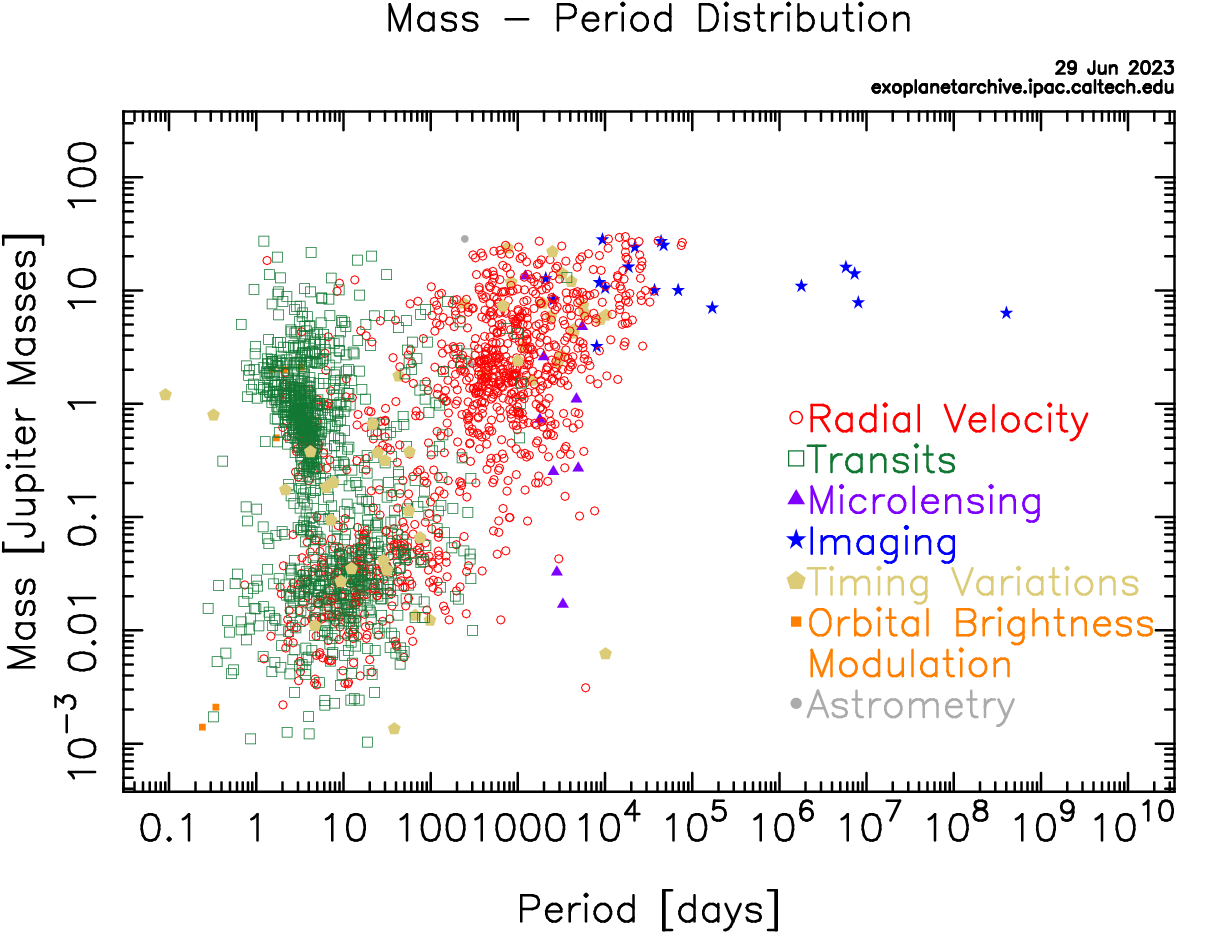
\includegraphics[width=0.95\textwidth]{intro/exo_massperiod.png}
  \end{center}
  \caption{The mass-period distribution of known exoplanets on the 
  NASA Exoplanet Archive on Jun 29th 2023
  \citep{akesonNASAExoplanet2013}. The plot is taken from the Archive
  itself which remakes the plot every time a planet is added.}
  \label{fig:archive_exoplanet_distribution}
\end{figure}

There are many different ways to detect an exoplanet, all of which provide
different information on the planet and are biased towards certain kinds of
planets. An easy way to see this is \Cref{fig:archive_exoplanet_distribution},
which plots all published exoplanets that have been added to the NASA Exoplanet
Archive, a database to that contains the information on all published
exoplanets, at the time of writing. Each detection method covers a different
range of periods and masses in the figure, representing the kinds of planet
planets the detection method is biased towards.

There are two broad forms of exoplanet detection, direct and indirect. Direct
detection of an exoplanet requires light to be collected from the planet itself
whereas indirect detection of an exoplanet is when the planet can be inferred
based on the star's light. The techniques that are relevant to this work are
direct imaging, radial velocity, transit, and astrometry. The transit technique
has detected the most planets. Currently, the NASA Exoplanet Archive has 4114
planets detected via transit, 1044 detected via radial velocity, 67 detected
with imaging, and 2 detected with astrometry. These numbers are steadily
increasing and missions such as TESS and Gaia will increase the number of known
exoplanets by the thousands \citep{Perryman2018a} \citep{Huang2018}.

\subsection{Indirect Detection} 

The first unambiguous exoplanet detection occurred in 1995 through radial
velocity observations of the star 51 Peg \citep{mayorJupitermassCompanion1995}.
The radial velocity method works by observing the Doppler shift in a star's
spectral lines and inferring the motion of the star around a planet-star center
of mass. This method is biased towards massive planets on edge on orbits as the
strength of a radial velocity signal is determined by the factor $M\sin{i}$,
where $M$ is the planet's mass and $i$ is the inclination of the planet's
orbit. The transit photometry exoplanet detection technique finds planets by
carefully monitoring the light coming from planets and watching for dips that
occur when a planet passes in front of the star. The radius and orbital period
of an exoplanet can be determined with this technique and it is therefore
biased towards large radius planets that are close to their star. The
astrometry detection method is done through extremely precise measurements of a
star's position in the planet of the sky \citep{Perryman2018a}. With the
precise movement of the star the corresponding motion of the planets can be
inferred.


\subsection{Direct Detection}

Direct detection of exoplanets is the process of collecting light directly from
the exoplanet. This can be done when the planet is hot enough to emit light on
its own or when light from the star reflects off of the planet. Direct
detection is biased towards large radius planets at wide separations. Because
of this direct imaging complements the other techniques by broadening the range
of orbital periods that we are able to detect, as can be seen in the upper
right part of \Cref{fig:archive_exoplanet_distribution}. A further benefit of
direct imaging is its ability to obtain detailed spectral information on
planets that are not detectable via the transit technique. Gathering spectral
information is of primary interest because it allows us to study the atmosphere
of the planet and search for signs of water and biosignatures.

\section{Method Outlook}
\label{sec:EPRV_HWO}

This dissertation will focus on the synergy of using radial velocity data to
predict the best times to make observations of exoplanets with a direct imaging
instrument. This combination was chosen due to the extreme difficulty of
getting spectral information on Earth-like exoplanets. The 2020 decadal report
recommended a 6 meter space-based telescoped optimized for directly detecting
and spectrally characterizing habitable exoplanets
\citep{nationalacademiesofsciencesPathwaysDiscoveryAstronomy2021} based on the
HabEx and LUVOIR mission concept studies
\citep{gaudiHabitableExoplanetObservatory2020,TheLUVOIRTeam2019}. Both the
HabEx and LUVOIR teams recommended considerable effort be put into finding
habitable worlds through other detection methods before the launch of a
space-based direct imaging mission. The main reason for this is simply that it
is easier to detect a planet when you now approximately where it will be.
Additionally, if a star is observed and no Earth-like planet is found then that
star can be removed from the direct imaging mission's list of stars to observe,
or target list. 

Earth-like planets around Sun-like stars are difficult to detect for any
method. They have a very low probability of transiting, astrometry detection of
an Earth-like planet can only be done with a space-based mission two orders of
magnitude more sensitive than the Gaia mission, and the radial velocity method
is similarly approximately two orders of magnitude
away\citep{gaudiHabitableExoplanetObservatory2020}. However, the radial
velocity method can feasibly make the required improvements with ground based
observatories and many efforts to reach the required sensitivity are in
progress\citep{Fischer2016a}. The radial velocity precision required to detect
an Earth-like planet is approximately 10 cm/s and a number of instruments have
recently demonstrated on-sky radial velocity precision under 1 m/s
\citep{maroonx2021, guptaTargetPrioritization2021,Pepe2021}. Additionally, the
Extreme Precision Radial Velocity initiative report from 2021 concluded that
there are multiple plausible system architectures that can detect Earth-like
exoplanets under the right conditions\citep{Crass2021}.

\section{Yield modeling}
\label{sec:intro_yield_modeling}

In studying future missions, an early step is to have some estimate of what
kind of science can be accomplished by the mission. This leads to the idea of
"yield modeling", methods that can compare different mission designs to
determine a trade space between cost and what kind of science a mission can do.
For exoplanet direct imaging, yield is typically treated as the number of
planets that can be detected
\citep{brownSingleVisitPhotometric2005,savranskyAnalyzingDesignsPlanetFinding2010,
starkMaximizingExoEarthCandidate2014}. Yield modeling plays an important role
in the mission design process and studies have looked at how many different
mission design choices impact exoplanet yield: precursor knowledge
\citep{morganFasterExoEarth2021}, the starlight suppression system
\citep{savranskyAnalyzingDesignsPlanetFinding2010,morgan19, Stark2016},
aperture size \citep{starkLowerLimitsAperture2015}, planet population
\citep{savranskyComparisonAnalyticalDepth2016}, and more. 

It is impossible to separate the work of exoplanet observation scheduling and
the science yield of an exoplanet mission. When simulating a mission to
establish the number of planets that can be detected there must be some choices
made to determine what order stars are observed in. The trade space is
effectively: what star should be observed, at what time, for how long. Because
direct imaging depends on reflected light there are considerable portions of an
exoplanet's orbit when it is not detectable so the choice of when to observe a
star is vital to whether an exoplanet is detected. Without simulating the full
process it cannot be proven that a mission will be able to make observations at
the most advantageous times for all target stars. In this manner yield modeling
and observation scheduling are inherently linked and important for mission
design.


\section{Dissertation Overview}
\label{sec:dis_overview}

In this dissertation I present what I have done to improve our chances of
directly imaging an exoplanet that has been detected with the radial velocity
method. In \Cref{cha:first_paper} I begin by analyzing what orbital information
is missing from a radial velocity fit, how to fill the information, how to use
that information to estimate the probability of a telescope directly detecting
that planet, and what can go wrong when doing so. Then in \Cref{cha:coupling} I
describe a method to accurately estimate what the dimmest planet a direct
imaging mission can detect in the likely scenario where the planet's brightness
has a subtle impact on the amount of observational noise. With that method in
\Cref{cha:accurate_pdet} to expand the probability of detection method to
incorporate more factors to describe more realistic observation scenarios. Then
in \Cref{cha:sim_and_scheduling}, I validate the probability of detection
calculations with a software tool I created that manages the creation of
synthetic planetary systems, the radial velocity observation process on the
synthetic planetary systems, full orbital fitting of the collected radial
velocity data, calculating the probability of detecting the synthetic planets
that were fitted, scheduling observations based on the probability of
detection, and finally simulating direct imaging observations based on the
created schedule to determine its yield.




\chapter{Scheduling Direct Imaging Observations Based on Radial Velocity Orbital Fits: Best Practices for Translating Orbits and Failure Modes}
\label{cha:first_paper}
This chapter is adapted from the paper \citet{spohnSchedulingDirect2022}.
\section{Introduction}%
% \label{sec:introduction}
To increase the number of planets they can detect, direct imaging mission concepts, such as LUVOIR
\citep{TheLUVOIRTeam2019} and HabEx \citep{gaudiHabitableExoplanetObservatory2020}, are planning on using precursor information
from other exoplanet detection methods.  In their science and technology definition study, the HabEx
team identified extreme precision radial velocity (EPRV) as the most promising way to make precursor
observations  \citep{gaudiHabitableExoplanetObservatory2020}.  The study noted that one issue with orbital fits from radial velocity
(RV) measurements is that they can lose accuracy, or grow ``stale'', with time, but this effect has
not yet been fully quantified.  In this paper we aim to establish metrics that indicate when an RV
fit is no longer useful or is actively harmful in planning a direct imaging mission.

While fitting an orbit to an RV curve can be done in many ways, over the past 20 years the two
primary methods have been gradient descent and Bayesian Hierarchical modeling.  Gradient descent has
focused on using the Leveneberg-Marquardt (LM) algorithm \citep{Levenberg1943b, Marquardt1963b} and
the most common method for Bayesian modeling is the Markov Chain Monte Carlo (MCMC) method
\citep{Metropolis1953, Hastings1970}.  Currently, the most commonly used tools are based on
the MCMC method because it excels at fitting data with large uncertainties \citep{Wright2009b}.
Among the most popular radial velocity fitting software is \code{RadVel} \citep{fultonRadvelRadialVelocity2018}, which provides an
open-source and flexible implementation of this method.

The fits generated from RV signatures provide a lot of information that can be directly used for direct
imaging, such as the planet's period ($T$), eccentricity ($e$), and argument of
periastron ($\omega_p$).  However, the fits are unable to separate the planet's mass ($M_p$) and
inclination ($i$), instead fitting only the quantity $M_{p}\sin{i}$.  Because of this ambiguity,
making probabilistic statements on when a planet will be detectable relies on sampling from priors
on inclination or planet mass.

When an RV signature has negligible error, which is largely based on our understanding of stellar
variability, the orbital fit will give accurate estimates of times when a planet will be within a
direct imaging instrument's geometric constraints (i.e., falling between its inner and outer working
angles). An inaccurate fit's larger error bars, combined with the inherent RV ambiguity on mass and
inclination and the lack of photometric information (the exoplanet's radius, albedo, and phase
function), makes predicting when the exoplanet will be detectable very difficult.

Due to their low mass, the RV signatures of Earth-like exoplanets have amplitudes on the order of
tens of centimeters per second.  The current state-of-the-art RV measurements mostly have precisions
of around 1 m/s \citep{EPRV2020}, making them incapable of detecting Earth-like exoplanets.
The 1 m/s noise floor is due primarily to inter-night stellar variability, and higher precisions for single
night observations have been demonstrated by instruments such as ESPRESSO \citep{Pepe2021} and
MAROON-X \citep{Seifahrt2021}.  The EPRV initiative is targeting precision of a few
cm/s \citep{EPRV2020} in the next 10-15 years. 

In Section~\ref{sec:consistent_orbits} we look at four different methods of constructing
orbits that are consistent with the radial velocity curve, discuss desired performance, and
analyze the differences between the methods in Section~\ref{sec:construction_method_analysis}. To
quantify these differences we establish two modes of failure in Section~\ref{sec:fitting_failure},
and in Section~\ref{sec:failure_results} we simulate the full process of gathering RV data, fitting
the data with \code{RadVel}, constructing orbits using the four different methods, and propagating
the constructed orbits in time to see when they fail.

\section{Constructing consistent orbits}%
\label{sec:consistent_orbits}

The general procedure of constructing populations of orbits consistent with RV measurements is:
\begin{enumerate}
    \item Define a ground truth planet and a $1 \sigma$ error (representing both observatory and stellar
        noise) on RV measurements.
    \item Create synthetic RV observations of the ground truth planet with the assumed errors.
    \item Fit the synthetic RV observations with \code{RadVel}.
    \item Use \code{RadVel} outputs to sample many orbits consistent with the RV signal.
\end{enumerate}

\subsection{Synthetic RV data}%
\label{sec:synthetic_RV_data}

To create synthetic data we define the ground truth planet with a semi-major axis ($a$),
eccentricity ($e$), the planet's argument of periastron ($\omega_p$), inclination ($i$), planet mass
($M_p$), stellar mass ($M_s$), and true anomaly of the planet at the first moment of the simulated RV
campaign ($\nu_{p_0}$). We compute the planet's radius using the model from
\citet{savranskyExplorationDynamical2019} which is a modification of the \code{Forecaster} model \citep{chenProbabilisticForecastingMasses2016}
focused on exoplanets likely to be found via direct imaging.

The semi-amplitude $K$ is calculated using equation 2.27 from \citet{Perryman2018a}
\begin{equation}\label{eq:K}
    K = \left( \frac{2\pi G}{T}\right)^{1/3} \frac{M_p \sin(i)}{M_s^{2/3}} \frac{1}{\sqrt{1-e^2}} \,,
\end{equation}
where $T$ is the planet's orbital period, $G$ is the gravitational constant, and assuming the
approximation that $M_s+M_p \approx M_s$. 

All simulated RV curves in this work are based on the RV measurements of Gliese 849 b from the
HARPS database between 2004 and 2012 \citep{Mayor2003a}. To mimic the cadence of observations we
calculate the average number of RV observations per month, $\lambda $, from our dataset. With
$\lambda $ as the expected separation in time of observations we sample a Poisson distribution for every
month between the start of 2000 and the start of 2010 to get a discrete number of observations in
each month. Within each month the observation times are distributed according to a random uniform
distribution.

At those synthetic RV observation times we calculate the true anomaly of the star, $\nu_s$, with
Newton-Raphson root-finding \citep{Murray2000}.  The radial velocity, neglecting barycenter motion, can then be found
as \citep{Perryman2018a}
\begin{equation}
    v_s = K \left(e \cos(\omega_s) + \cos(\nu_s + \omega_s)\right) \,,
\end{equation}
where $\omega_s$ is the star's argument of periastron, equal to $\omega_{p}+180\degree$.  This
process is repeated at every observation time to create the ``true'' radial velocity signature of
the planet over a set range of time.  To simulate noise on the observations, we draw the
``observed'' RV value of each observation from a normal distribution with the mean at the true
radial velocity value and the $1 \sigma$ error equal to the defined $1 \sigma $ error which
represents observatory and stellar noise. Note that there are many different potential sources of
error on RV measurements \citep[see, e.g.,~][]{Fischer2016a}, which we are combining into a single
$1 \sigma $ value to match the assumed inputs to \code{RadVel}, which are a time series of observed
radial velocities and their $1 \sigma $ values. To be clear, the defined 1 $\sigma $ error
is not based on a specific instrument or noise source, but rather represents a
simplified parameter that can be varied in order to test the effects of
different RV precisions.


\subsection{Fitting the RV curve}%
\label{sec:rvfit}
We use \code{RadVel} \citep{fultonRadvelRadialVelocity2018} to create an
orbital fit from our noisy, synthetic data. The fitting basis used is the
\code{RadVel} standard for fitting: $T$, $T_c$ (time of conjunction),
$\sqrt{e}\cos{\omega_s}$, $\sqrt{e}\sin{\omega_s}$, $K$.  Gaussian priors are
assigned to $T_c$ and period $T$. To simulate imperfect information about the
planet we offset the Gaussian priors used by \code{RadVel} for $T$ and $T_c$.
This is done by sampling a normal distribution centered on the true mean with a
1$\sigma$ error of 10\% of $T$. This prior assumes that $T$ and $T_c$ can be
determined in part based on analysis of the RV time series before using
\code{RadVel}. A Nelder-Mead \citep{Nelder1965,Gao2010a} optimization is then
run on the posterior to refine it. Then the fitting is done using the
\code{RadVel} implementation of the MCMC package \code{emcee} \citep{emcee}.
The MCMC analysis provides the fitting basis parameters and the likelihood
associated with each step of the Markov Chain.

\subsection{Transforming Fitting Basis to Keplerian Elements}
To simulate imaging observations we need to be able to propagate in time and find the separation and
brightness at any time step. Because of this we must calculate the Keplerian orbital parameters
that were defined to create the synthetic RV data shown in Section~\ref{sec:synthetic_RV_data} 
The eccentricity $e$ is given by 
\begin{equation}
     e = \left( \sqrt{e} \cos(\omega_s) \right)^2 + \left( \sqrt{e} \sin(\omega_s) \right)^2
\end{equation}
and the argument of periastron is given by
\begin{equation}
    \omega_s = \arctan\left(\frac{\sqrt{e} \sin(\omega_s)}{\sqrt{e} \cos(\omega_s)}\right) \,,
\end{equation}
with $\omega_p = \omega _s + 180\degree$. The time of periastron requires
several more intermediate calculations.  Using the geometry shown in Figure 1
of \citet{fultonRadvelRadialVelocity2018} we can express the true anomaly of
the planet, $\nu_p$, at the time of conjunction as
\begin{equation}
    \nu_p = 90\degree - \omega_s \,.
\end{equation}
With this we can find the eccentric anomaly of the planet at the time of conjunction as
\begin{equation}%
    \label{eq:ecc_anom}
    \tan \left( \frac{E}{2}\right) = \sqrt{\frac{1-e}{1+e}} \tan \left(\frac{\nu}{2}\right)
\end{equation}
and solve for the mean anomaly at that time with Kepler's equation
\begin{equation}%
    \label{eq:mean_anom}
    M = E - e \sin{E} \,.
\end{equation}

We find the time of periastron passage as
\begin{equation}
    T_p = T_c - \frac{M}{n} = T_c - \frac{M T}{2\pi}
\end{equation}
where $n$ represents the orbital mean motion.
The semi-major axis ($a$) is a function of the period and gravitational parameter $\mu=G M_s$ (again using
the approximation $M_p + M_s \approx M_s$)
\begin{equation}
    a = {\left( \mu {\left(\frac{ T}{2\pi}\right)}^2 \right)}^{1/3} \,.
\end{equation}
Using equation~\ref{eq:K} we can calculate the quantity $M_p\sin{i}$ based on the fit values of $K$,
$e$, and $T$. However, the $M_p \sin{i}$ quantity cannot be separated into $M_p$ and $i$ without
making further assumptions.

\subsection{Methods of constructing consistent orbits}\label{sec:orbit_methods}
Since the end goal of this work is to analyze how well RV data can be utilized for planning direct imaging observations we
need a metric based on an RV signal that quantifies when a planet will be detectable for a direct
imaging instrument.  Our approach is similar to the calculation of completeness for planetary
populations \citep{brownObscurationalCompleteness2004,
brownSingleVisitPhotometric2005, brownNewCompletenessMethods2010,garrettAnalyticalFormulation2016}.
This approach relies on constructing a
large set of orbits that a planet could be on and describing the probability of making a detection
as 
\begin{equation}\label{eq:prob_det}
    P_{\textrm{det}}(t) = \frac{\textrm{Number of orbits detectable at time $t$}}{\textrm{Number of
    constructed orbits}}
.\end{equation}
Unlike Brown, we are basing the orbits on prior information from the RV curve gathered from the 
\code{RadVel} fit, rather than drawing from assumed distributions of parameters describing some population
of planets.

Currently, there is no single universally agreed upon method to create the large set of orbits
necessary for Equation~\ref{eq:prob_det} to give reliable results. To fill that gap we have analyzed
four different ways of using \code{RadVel}'s outputs for that purpose. Ideally, the set of orbits
generated will lead to accurate predictions of when the planet is detectable while avoiding
predictions that the planet will be detectable when it isn't.

Each of the methods, described below, begins by generating values for $a$, $e$, $\omega_p$, $T_p$, and $M_p \sin
i$ and then sampling a prior distribution on $i$ to separate the planet mass and inclination.
\subsubsection{Maximum Likelihood}
In this method we take the fitting basis parameters ($T$, $T_c$, $\sqrt{e} \cos{\omega_s}$, $\sqrt{e}
\sin{\omega_s}$, $K$, as described in Section \ref{sec:rvfit}) from the MCMC step with the highest likelihood.
This means that the only source of variation in the constructed orbit population comes from sampling
the prior on $i$ to split up the $M_p \sin i$ quantity.

\subsubsection{Maximum Kernel Density Estimate (KDE)}
The kernel density estimate of the fitting basis is found using Scott's method \citep{Scott1992}.
We then use the Broyden–Fletcher–Goldfarb–Shanno (BFGS) minimization routine
\citep{Nocedal2006}, as implemented in SciPy
\citep{virtanenSciPyFundamental2020}, to find the parameter set that maximizes the kernel density
estimate. Like the maximum likelihood method above, this creates a single set of parameters from the
fitting basis and all variations are in $i$ and $M_p$ due to sampling the inclination prior.

\subsubsection{Credible Interval}
\code{RadVel} defines a ``Credible interval'' for a parameter as the median and standard deviation of the
fitting basis parameters for every step taken during MCMC analysis. 
This method takes that same approach, calculating the median and standard deviation for each
fitting basis parameter based on every step of the MCMC analysis.
Then to create orbits we sample each fitting basis parameter independently, treating each as normally distributed based on their median and standard deviation. Unlike the previous two methods of
generating orbits, this one has variation in all orbital parameters, as well as inclination and planet mass.

\subsubsection{Multivariate Gaussian}
To get a distribution of high likelihood orbital parameters, the MCMC steps are sorted by likelihood
and the fitting basis parameters of the top 1000 are selected, from the hundreds of
thousands of MCMC steps, to compute a covariance matrix. We found that 1000 steps were enough to
identify the high likelihood regions while keeping computation times low. Using the
covariance matrix of MCMC parameters we can construct new sets of fitting basis parameters by
sampling a multivariate Gaussian. Sampling in this way lets us generate many more high
likelihood parameter sets than the chains alone provide without disregarding correlations between
the fitting basis parameters, most notably the relationship between $T$ and $T_c$. Like the credible
interval method above, this results in many different combinations of orbital parameters.

\subsection{Inclination Sampling}%
\label{subsub:inclination_sampling}
For each parameter set created by the methods described above, the inclination and mass ambiguity is
explored by sampling from the inclination distribution. Using the isotropic orbit orientation
assumption described in \citet{Savransky2011a} the inclination is distributed sinusoidally between
$0$ and $\pi$ radians, such that $i \sim \cos^{-1}\left(U\right)$ where $U$ represents a uniformly
distributed random value between -1 and 1. Further, we can impose certain constraints onto the mass
that narrow the inclination space. As $\sin{i}$ goes to 0, the planet's mass goes to infinity so we
impose restrictions on what inclinations are possible. Depending on a stellar object's chemical
composition it will begin hydrogen burning when its mass is above $\sim 0.07-0.09 M_{\odot}$
\citep{Perryman2018a}, at which point the object is no longer classified as a planet.  We use
the median point in that range to define a critical inclination
\begin{equation}
    i_{crit} = \arcsin\left(\frac{M_p \sin{i}}{0.08 M_{\odot}}\right) \,.
\end{equation}
To find a distribution of potential inclinations we sample from the prior sinusoidal distribution,
limited by $i_{crit}$, and solve for the corresponding $M_p$ value for each
inclination. The planet's radius is calculated using the same method from
Section~\ref{sec:synthetic_RV_data}.

\subsection{Propagation in time}
The constructed orbits now have all the information necessary to simulate their motion.  Using the time of
periastron $T_p$ we can find the mean anomaly at each desired time step $t$
\begin{equation}
    M(t) = n (t - T_p)
\end{equation}
which is used as an intermediate step for the desired direct imaging parameters, the difference in
brightness magnitude between the planet and star ($\Delta\mathrm{mag}$) and the angular separation
between the planet and star ($\alpha$).  To find those we first calculate the planet's true anomaly,
$\nu_p$ from its mean anomaly using Equations~\ref{eq:ecc_anom}--\ref{eq:mean_anom}, again via Newton-Raphson. The orbital radius $r$ is given using the
equation
\begin{equation}%
    \label{eq:r}
    r = \frac{a \left( 1 -e^2 \right) }{1 + e \cos \nu_p } \;
.\end{equation}
Then we find the projected separation
\begin{equation}
    s = \frac{r}{4} \sqrt{4 \cos{2i} + 4 \cos{2\theta} - 2\cos( {2i-2\theta} ) - 2\cos({2i+2\theta}) + 12} \,.
\end{equation}
where $\theta = \nu_p + \omega_p $ is the argument of latitude of the planet.
From this and the distance to the star $d$, we calculate the angular separation
\begin{equation}%
    \label{eq:alpha}
    \alpha = \tan^{-1}\left( \frac{s}{d} \right)
.\end{equation}
The phase angle $\beta$ is calculated as
\begin{equation}%
    \label{eq:beta}
    \beta = \arccos( {-\sin{i}\sin{\theta}} )
\end{equation}
under the assumption that $d \gg r$ and that the observer is looking down on the orbital plane, as described in \citet{savranskyExplorationDynamical2019}.
The photometry calculations assume Lambertian scattering and use Lambert's phase function
\begin{equation}
    \Phi(\beta) = \frac{1}{\pi} \left( \sin\beta + (\pi-\beta) \cos\beta\right) \,.
\end{equation}
We find the flux ratio $F_R$, or the ratio of the planet's flux $F_p$ over the star's flux $F_s$,
as
\begin{equation}
    F_R = \frac{F_p}{F_s} = p\Phi(\beta)\left(\frac{R_p}{r}\right)^2 \,.
\end{equation}
For the purpose of these simulations all planets are assigned the Earth's geometric albedo $p$ of
$0.367$ as in \citet{Seidelmann2006}.
The difference in magnitude between star and planet, $\Delta\mathrm{mag}$, is
\begin{equation}
    \Delta\mathrm{mag} = -2.5\log_{10}F_R \,.
\end{equation}

\subsection{Orbit detectability}
With $\alpha$ and $\Delta\mathrm{mag}$ we can compare the visibility for each
planet against the constraints of the observatory to calculate visibility. A detectable planet will
meet the criteria
\begin{align}
    \text{IWA} < \alpha < \text{OWA}\label{eq:alpha_constraint}\\
    \Delta\mathrm{mag} < \Delta\mathrm{mag}_0\label{eq:dMag_constraint}
\end{align}
where IWA is the observatory's inner working angle, OWA is the outer working angle, and
$\Delta\mathrm{mag}_0$ is the observatory's limiting difference in brightness \citep[effectively equivalent to the instrument contrast capability---for further discussion see][]{Brown2005d}. Using these
constraints, the method of propagation, and equation~\ref{eq:prob_det} we can calculate the
probability of detection as a function of time.
\section{Construction method analysis}%
\label{sec:construction_method_analysis}
\begin{figure}[htpb]
    \centering
    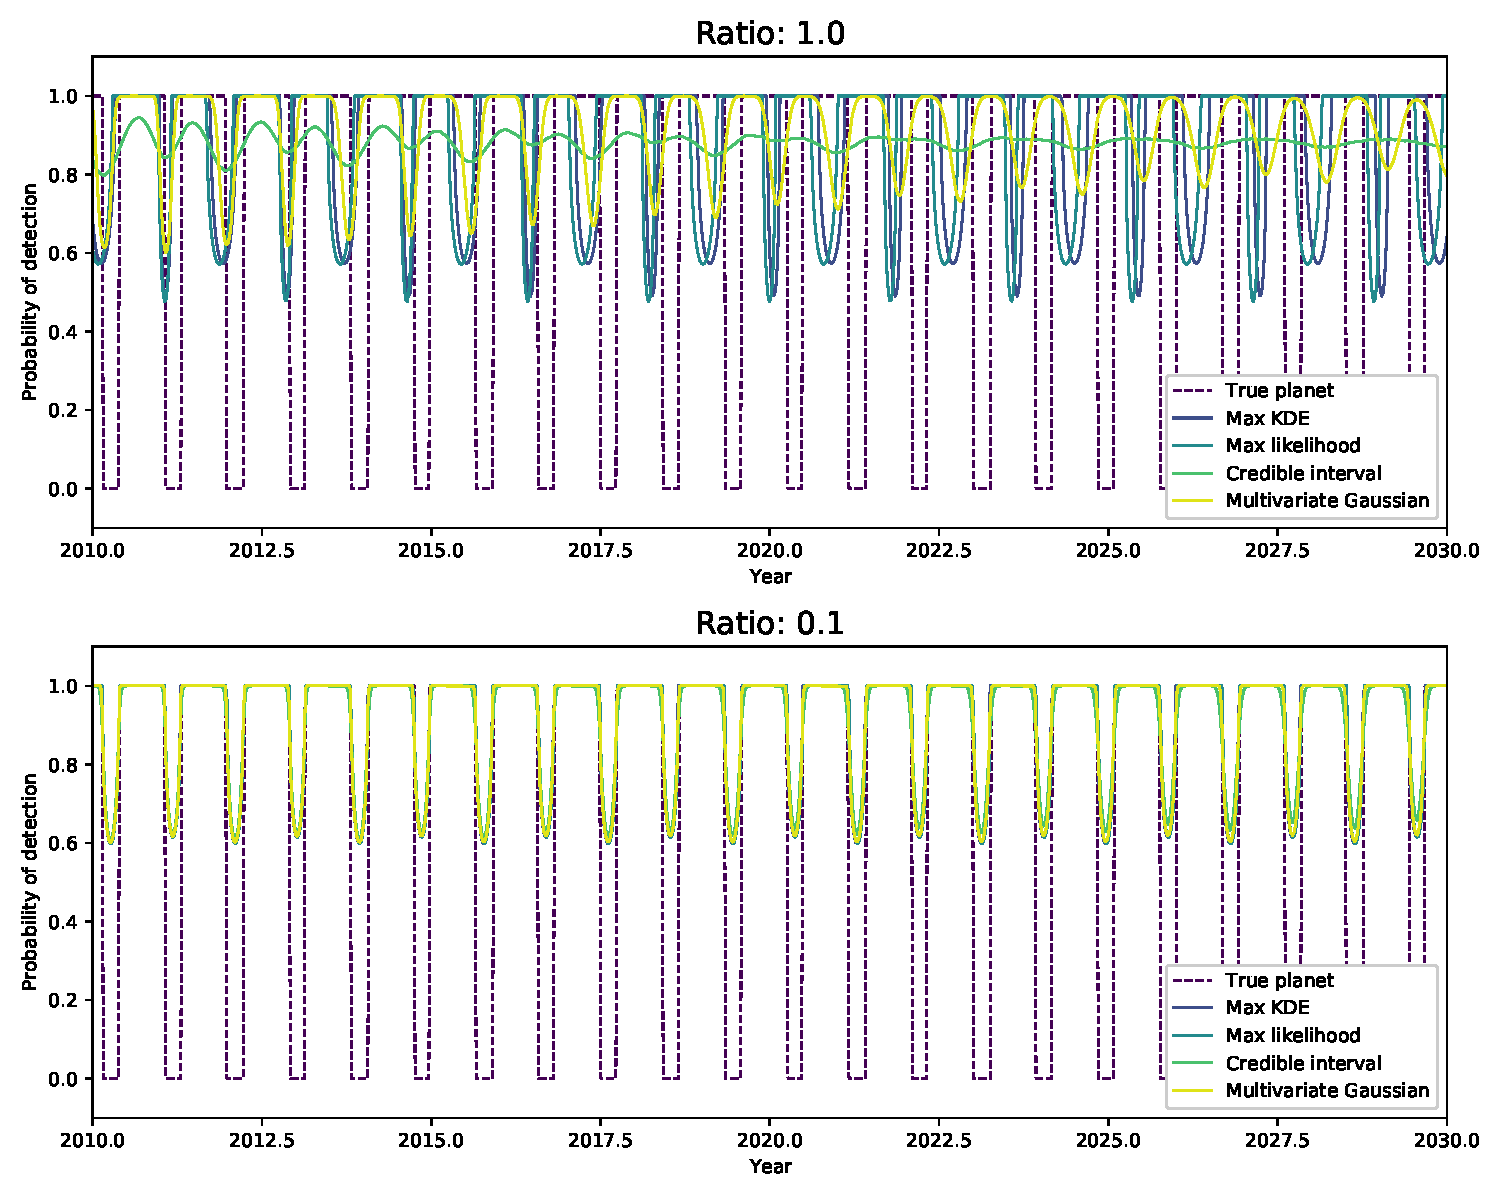
\includegraphics[width=\linewidth]{ch1/figures/prob_det_new.pdf}
    \caption{Comparison of how the four different orbit construction methods (max KDE, max
    likelihood, credible interval, and multivariate Gaussian) perform at calculating the
    probability of detection at two different ratios of RV error to RV semi-amplitude. The ``True
    planet'' line has a value of 1 when the defined planet is detectable by a HabEx-like instrument, and a value of zero when it is not.}%
    \label{fig:prob_det_comparison}
    %Note: the reason that 1.0 max L plot is so varied is because its e is 0.52
\end{figure}
\begin{figure}[hpt]
    \centering
    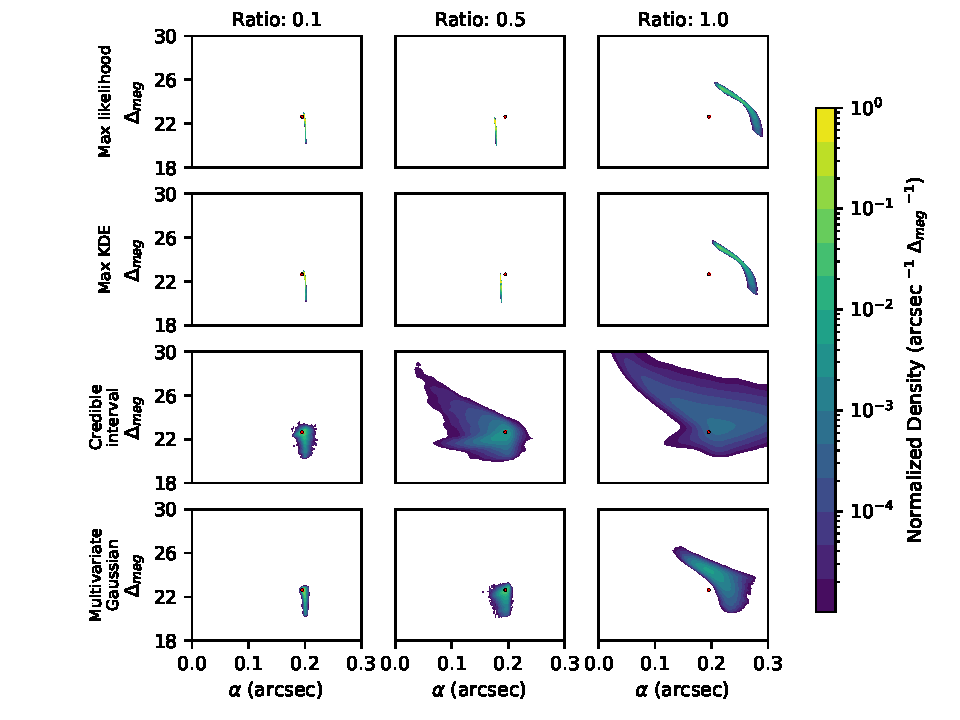
\includegraphics[width=\linewidth]{ch1/figures/construction_method_vs_error_100.pdf}
    \caption{Distributions in $\alpha $ vs $\Delta\mathrm{mag}$ space for the different orbit construction
    techniques at the time of fitting. The point represents the true planet's location. The planet
    has $a$ of 2 AU, $e$ of 0, $i$ of 100\degree, $R_p$ of $3.48 R_{\bigoplus}$, geometric
    albedo of 0.367, and is around a Sun-like star at a distance of 10 parsecs. Each column uses the
    same output from \code{RadVel} with a set ratio of RV error to RV semi-amplitude and assumes 10
    years of radial velocity measurements.}%
    \label{fig:construction_method_pdfs}
\end{figure}
\begin{figure}[htpb]
    \centering
    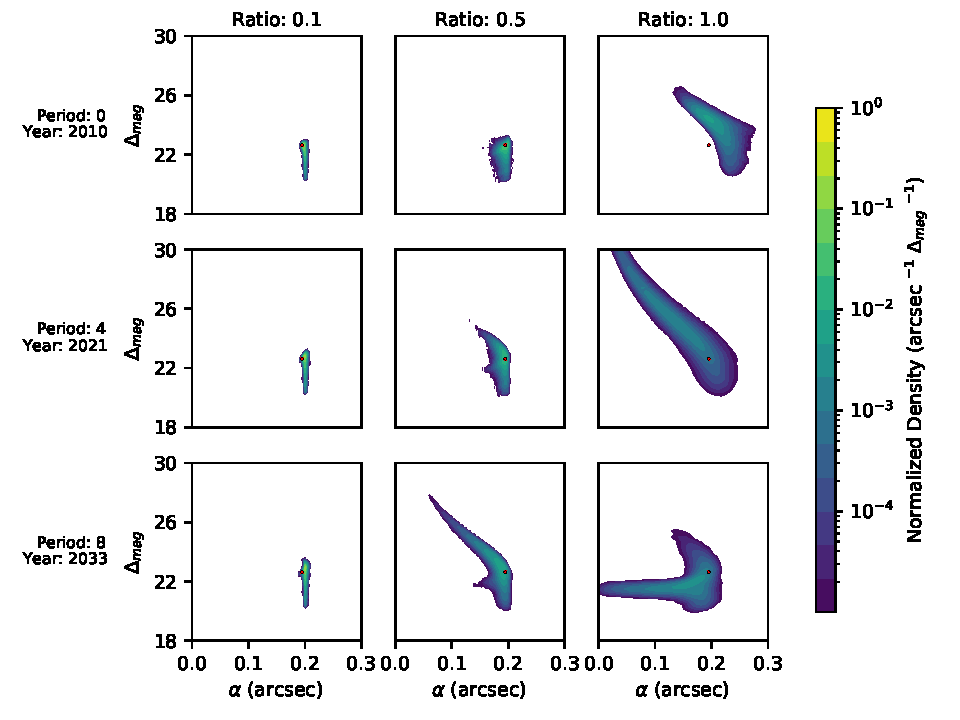
\includegraphics[width=\linewidth]{ch1/figures/dispersion_in_time_i100.pdf}
    \caption{Temporal evolution of orbits constructed with the multivariate Gaussian method shown in
    Figure~\ref{fig:construction_method_pdfs}.}%
    \label{fig:dispersion_in_time}
\end{figure}
We tested the different methods of creating consistent orbits laid out in
Section~\ref{sec:orbit_methods} using a super-Earth on an edge-on orbit, as shown in
Figure~\ref{fig:prob_det_comparison}. We see that there is not much difference between the
performance of the different construction methods when the ratio of error to semi-amplitude is low.
However, when the ratio is high the different construction methods diverge significantly in their
predictions of planet detectability.

The methods that create distributions of the fitting basis parameters (credible interval and
multivariate Gaussian) have their features decay in time.  This is especially clear for the credible
interval curve, which begins with a low amplitude wave that peaks while the true planet is visible
and decays to a nearly constant value after 10 years. That decay represents the predictive power of
the consistent orbits decreasing as time goes by. The multivariate Gaussian curve decays, but to a
lesser extent.  It no longer reaches a probability of 1 by the end of the 20 years, but still
has significant oscillations.  The two methods that rely on a single set of fitting basis parameters
(max likelihood and max KDE) never decay, but this leads to many times when the true planet is not
detectable while the predicted probability of detection is unity.

Differences in this decay are further explored in Figure~\ref{fig:construction_method_pdfs} which
shows the joint density of the angular separation-$\Delta _{\textrm{mag}}$ phase space for the
various construction methods for a planet with a close to edge-on orbit, ($i=100\degree$ ). Note
that this figure represents a single scenario of orbital parameters and will vary greatly depending
on the orbital parameters and the quality of the RV measurement data. The max likelihood and max KDE
methods produce very clustered orbits. In this scenario however (and in most scenarios as we show in
Section~\ref{sec:failure_results}), none of the distributions created by either max likelihood or
max KDE methods include the true planet. That will lead them to make inaccurate predictions for
detectability. The large spread shown by those two methods for the ratio of one is due to the max
KDE and highest likelihood fitting basis sets having high eccentricity which, combined with the
inclination sampling, produced a lot of variability in the separation-$\Delta \mathrm{mag}$ space.
The orbits constructed with the credible interval method show the largest overall variance. For
small error to semi-amplitude ratios, the orbits constructed with the credible interval method
cluster around the true planet's location, but the distribution rapidly grows in size as the ratio
increases.  
In this case the ``true'' planet remains in the high
density regions of the orbits constructed with the credible interval method. However, for ``true''
planets with higher inclinations this would not be the case because the prior on inclination
produces more edge-on orbits.  While the plots in Figure~\ref{fig:construction_method_pdfs} are for
a single, specific set of values for the planet and orbital parameters and stellar distance, they
can be easily scaled for any variation of the parameters.  The angular separation, as given in
Equation~\ref{eq:alpha}, scales nearly linearly (in the small-angle approximation) with both
semi-major axis (directly) and stellar distance (inversely). For changes in semi-major axis,
$\Delta\mathrm{mag}$ scales as $\Delta\mathrm{mag} - 5\log_{10}\left(\frac{a}{a_0}\right)$ where
$\frac{a}{a_0}$ is the ratio of the new to original semi-major axis. Changes in geometric albedo or
planet radius will similarly additively change the $\Delta\mathrm{mag}$ while not affecting the
angular separation.

In the scenario shown in Figure~\ref{fig:construction_method_pdfs}, the multivariate Gaussian orbit
construction method maintains a tighter density than the credible interval method while still
including the true planet for ratios 0.1 and 0.5, which the two max methods do not, but does not
include the true planet for a ratio of 1. Similar to the credible interval method, for large
inclinations the true planet will drift further away from the high density regions of the
distributions.

Figure~\ref{fig:dispersion_in_time} further explores the information decay in time, showing how the
orbits disperse at three different times.  In this case we use the multivariate Gaussian method, but
the plot has similar features for the credible interval method.  Each time corresponds to an integer
orbital period so that the true planet is at the same location along its orbit. For all three ratios
we see that the distribution disperses significantly in time.  Unsurprisingly, the spread in the
distribution is proportional to the assumed error ratio, with the lowest ratio showing little change
after even 8 full orbital periods (in this case 23 years). In every case except one the true planet
remains within a region where the orbit distribution has a normalized density above $10^{-5}$, but
clearly the predictive power of the orbits constructed from noisy RV fits decreases in time.

\section{Fitting failure}%
\label{sec:fitting_failure}

Having established methodologies for sampling orbits consistent with RV data, we can now evaluate
how well our different construction methods perform in scheduling direct imaging observations. A
successful orbit fit will show a high probability of detection when the true planet is visible, dip
when the true planet is not visible, and continue to do so consistently over many orbital periods.
We have identified two primary types of fitting failure, which we call intermittent failure and
dispersion failure. Intermittent failure occurs when an orbital fit indicates a high probability of
an observation yielding a detection at a time when the true planet is not detectable. Dispersion
failure occurs when the probability of detection curve flattens, at which point the orbital fit
gives little information on when an observation should be scheduled.

\subsection{Intermittent failure}%
\label{sub:intermittent_failure}
\begin{figure}[htpb]
    \centering
    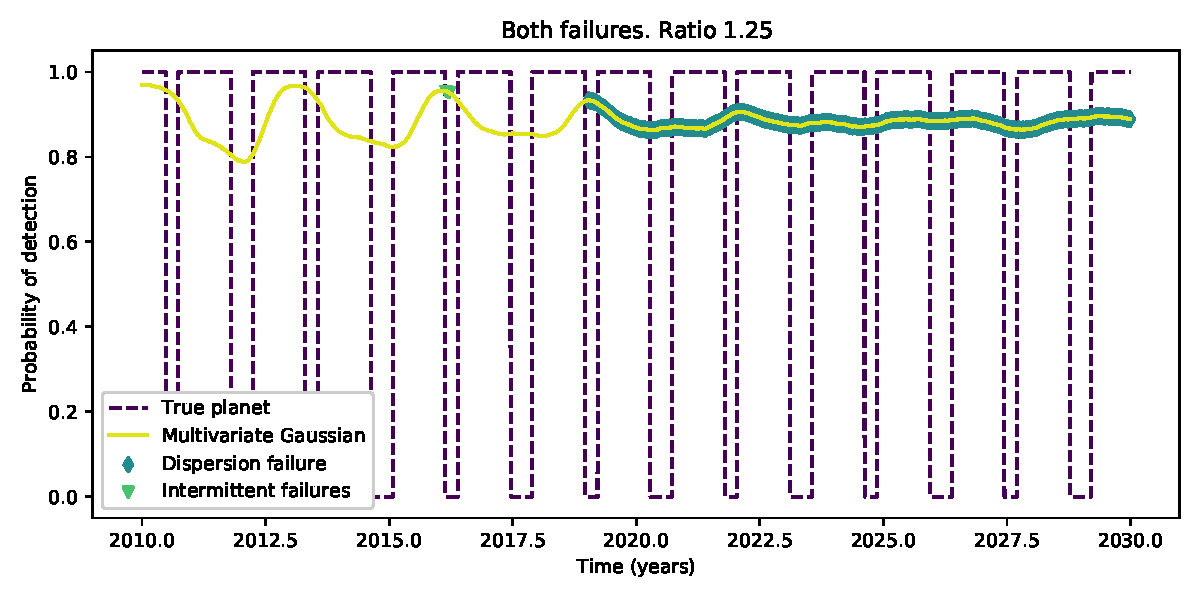
\includegraphics[width=\linewidth]{ch1/figures/prob_det_vs_time_both_failure.pdf}
    \caption{Probability of detection curve demonstrating both kinds of failure. The green triangles represent steps
    when all conditions for intermittent failures are met. The end of the curve, highlighted,
    represents the point in time when dispersion failure has occurred. This is a somewhat
    extreme example as it is unlikely that a planet with an error to semi-amplitude ratio of 1.25
    would be considered for observation.}%
    \label{fig:figures/both_failures}
\end{figure}
The point of intermittent failure is to identify times when a mission scheduler would plan an
observation with confidence even though it would lead to a null detection.
Figure~\ref{fig:figures/both_failures} shows a peak marked as an intermittent failure because it is a
high and relatively stable probability of detection at a time when the true planet is not visible.
Observing at that time would be seen as a good idea, but lead to a failed detection of a planet that
is detectable for the majority of the mission. Intermittent failure occurs when all of
the following conditions are met:
\begin{enumerate}
    \item The true planet is not detectable;
    \item The estimated probability of detection is in the top 90\% of the local probability of
        detection values;
    \item The probability of detection is changing by less than 0.0001 per day; and
    \item The previous three conditions hold for 1 day.
\end{enumerate}
Note that the numerical values given in the conditions have been used for this analysis and were
determined heuristically based on what we assume someone scheduling a direct imaging mission would
see as satisfactory information that an observation will result in a detection. For a specific
mission the values should be optimized based on the goals and constraints of that mission.

The first condition exists to focus on times when a scheduled observation would result in a failed
detection. Note that this condition makes it so that if a planet is always detectable, such as
face-on orbits, no orbital fit can produce an intermittent failure.  The second condition exists
because the orbit construction methods, primarily those that have multiple fitting basis parameters
such as credible interval and multivariate Gaussian, will produce probability of detection curves
that don't always reach unity, and additionally the peaks decay in time (as shown in
Figure~\ref{fig:prob_det_comparison}). By describing it in terms of a local range of values we avoid
restricting our observations to an absolute threshold that may not be met even though the detection
curve is peaking when the true planet is detectable. The second condition can be expressed as
$P_{\textrm{det}} > \left(0.9 \left(  \textrm{local max} - \textrm{local min}\right) + \textrm{local
min}\right)$.  The third condition exists because there are many times when the first two conditions
are met while a large percentage of orbits consistent with the RV observations are entering
or exiting the direct imaging instrument constraints, causing the probability of detection curve
to change rapidly. We assume that a mission scheduler would avoid such times, preferring to
observe when the number of orbits detectable is stable.
To demonstrate the relevance, without the third condition the curves in Figure~\ref{fig:prob_det_comparison}'s
bottom plot would be considered in intermittent failure immediately before the true planet becomes
detectable and immediately after it is not detectable, even though it is clearly better to observe
in the long time period when the probability of detection is stable at unity, not right before or
after that time period. The last condition exists to rule out the times when the first three
conditions are met for a time shorter than an observation would be scheduled for, which should be
tuned based on the required integration time of an observation.

To determine the local maxima required for the second condition we break the probability of
detection curve into different sections based on the extremum. The
first section begins at the initial time if the first extremum is a local maximum, or begins at the
first minimum if the first extremum is a local minimum. Then each subsequent section begins at each
subsequent minimum. The last section ends at the last minimum if the last extremum is a local
minimum, and the last point if the last extremum is a local maximum. Within each section, the local
probability of detection maximum is the greatest probability of detection in the section. To make
the peak finding robust we require the maxima to be at least 0.05 above the greater of the two
nearest minima, and the converse requirement was used for determining the minima. Lowering the 0.05
number will make the metric describe flatter regions, which better describes complete dispersion.
However, there is little reason to lower it because in situations when the probability of detection
is varying by less than 0.05 the orbits are so dispersed that the orbital fit is not providing
useful information about when to schedule observations, which is captured by the second failure
metric called dispersion failure.

\subsection{Dispersion failure}% 
\label{sub:dispersion_failure} 

Dispersion failure occurs when the probability of detection curve flattens to the point where a full
orbital period passes without any extrema, for the probability of detection curve as defined above.
Figure~\ref{fig:figures/both_failures} shows dispersion failure occurring 9 years after the
collection of the data used for the orbital fit.  If the constructed orbits have a wide range of
orbital parameters the probability of detection curve will show little change from the beginning,
such as the ``Credible interval'' curve for a ratio of 1 in Figure~\ref{fig:prob_det_comparison}.
The primary cause of dispersion is from many constructed orbits having different periods, making the
initial cluster of orbits disperse quickly.  Past the point of dispersion failure, there is no reason
for a mission scheduler to favor one point in time for observation over another, based on the
information from an RV fit.

\section{Failure results}%
\label{sec:failure_results}
\begin{figure}[htpb]
    \centering
    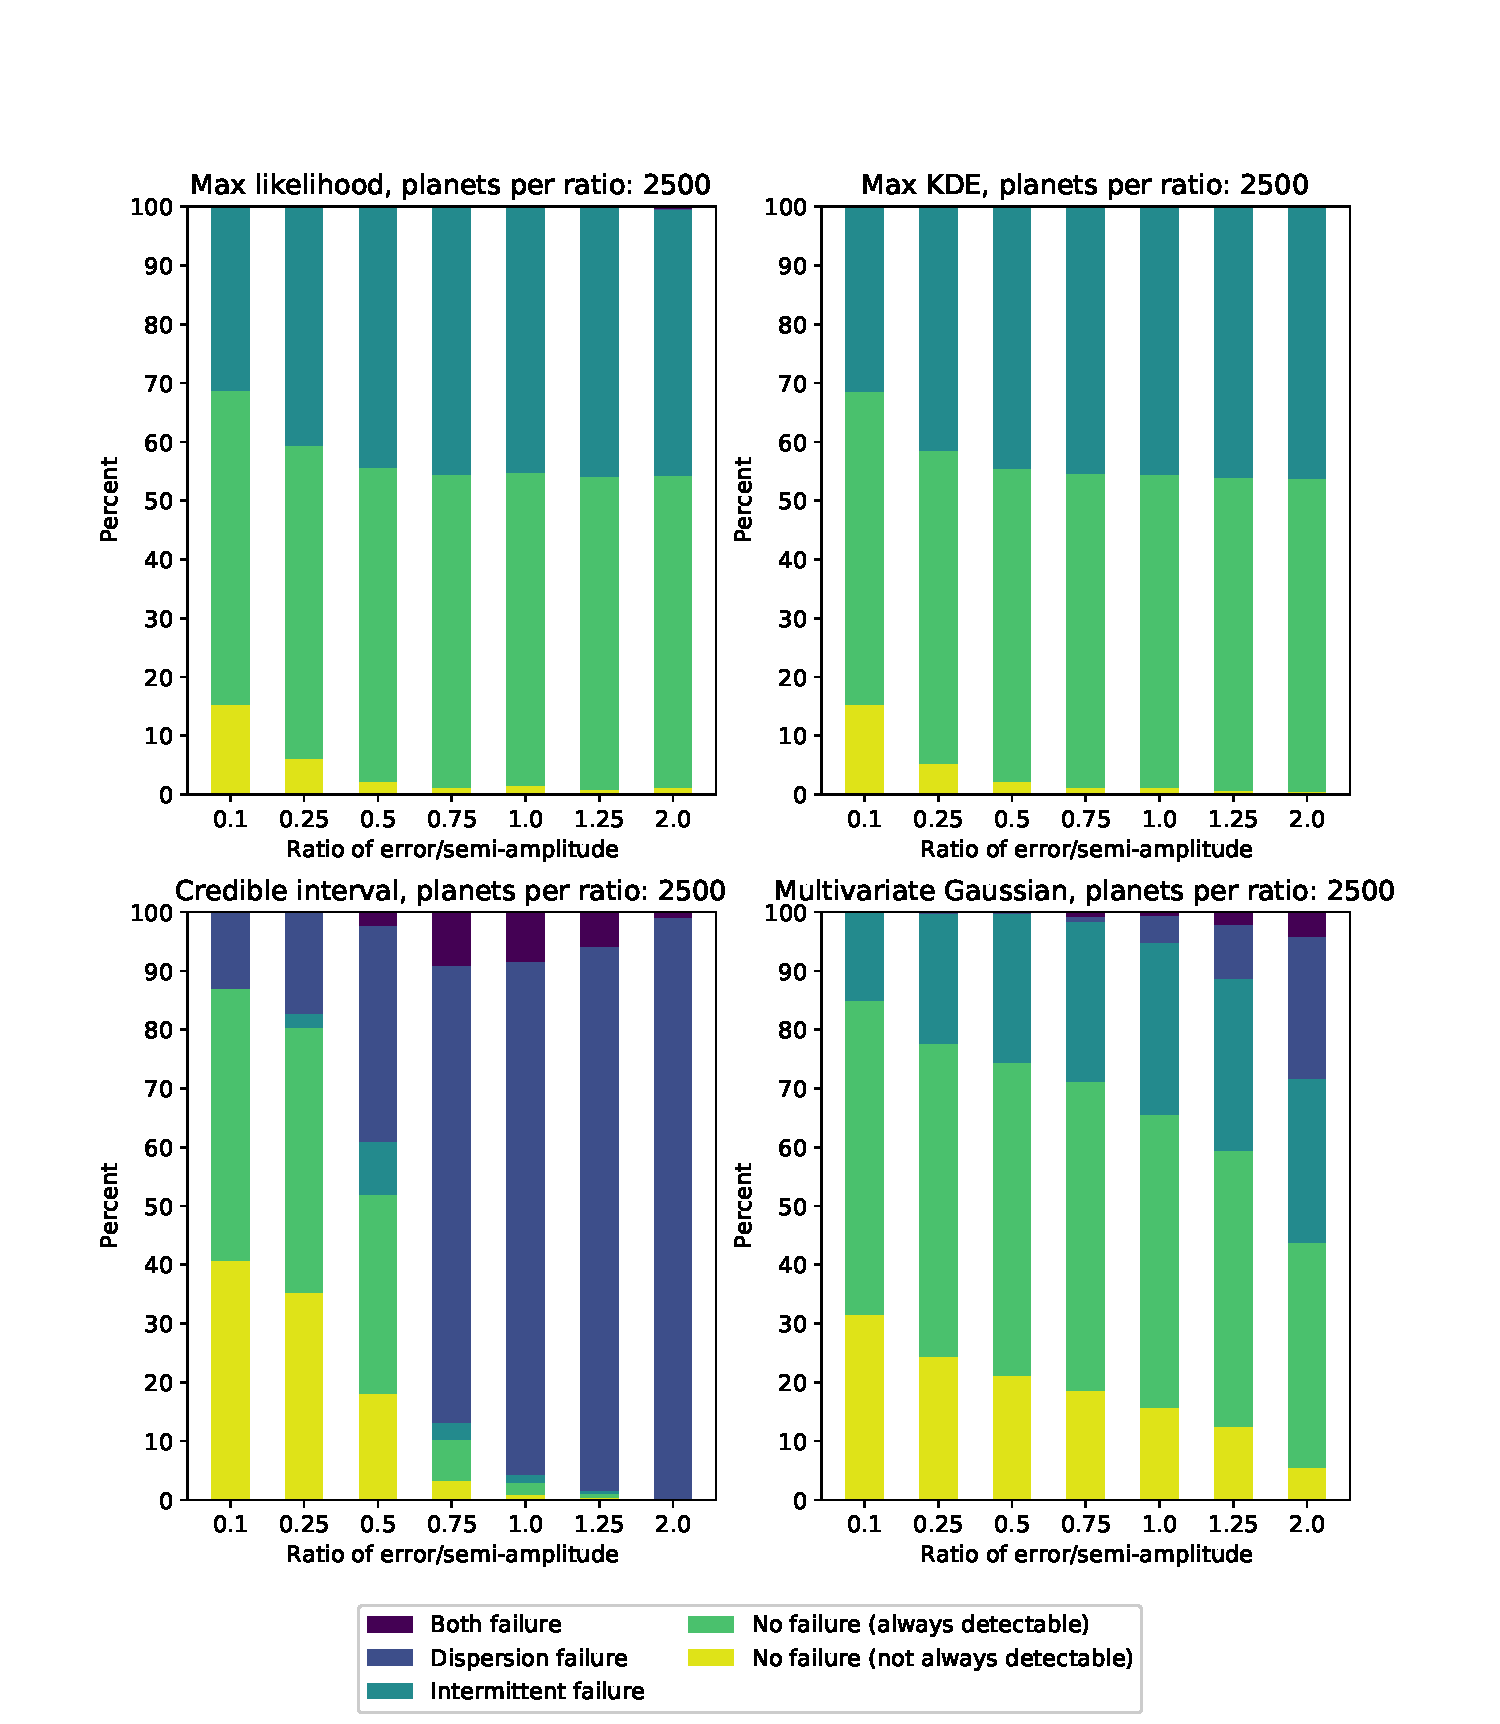
\includegraphics[width=\linewidth]{ch1/figures/construction_method_bars_including_always_detectable.pdf}
    \caption{Failure mode statistics for the four different construction methods for different
        ratios of RV error to signal semi-amplitude. We see that the failure percentage increases at
        different rates for each construction method as the ratio of error to semi-amplitude
        increases. Max likelihood and max KDE perform poorly for all ratios tested.  Credible
        interval performs the best for very low ratios and multivariate Gaussian significantly
        outperforms credible interval for ratios of 0.5 or greater. Note that while max likelihood
        and max KDE appear to perform well, this is only the case when the planet is always detectable
        which makes it a trivial result.}%
    \label{fig:con_method_bar_comparison}
\end{figure}
\begin{figure}[htpb]
    \centering
    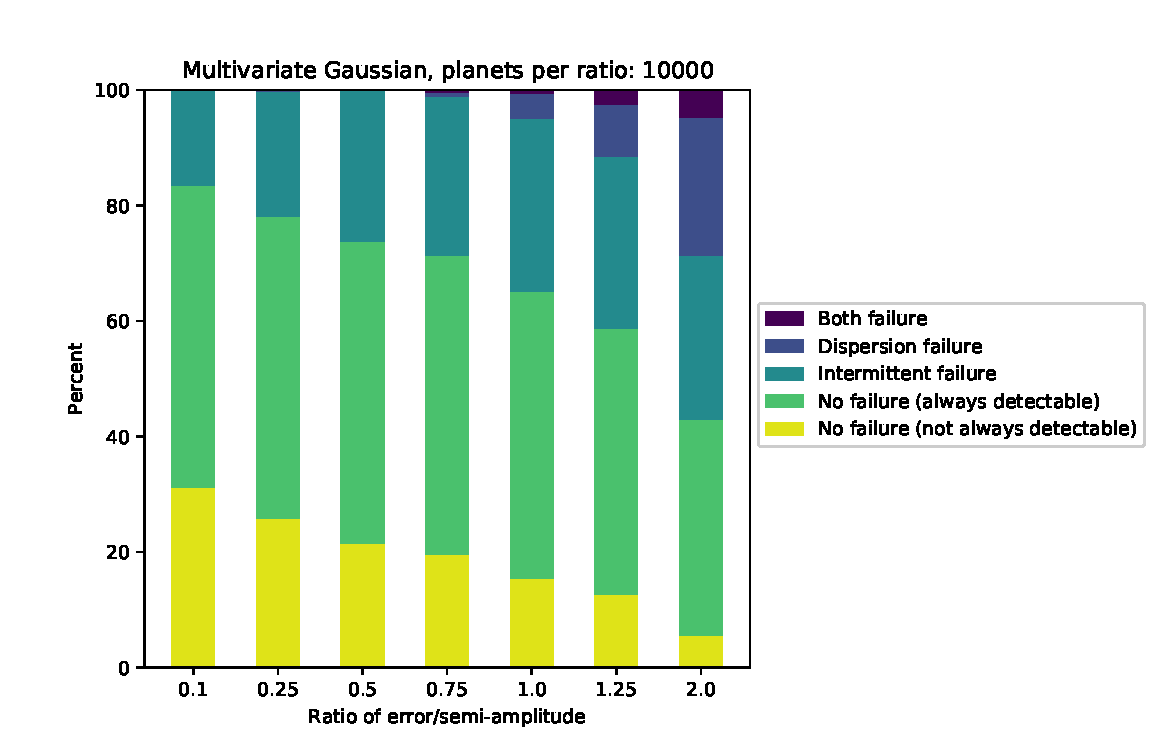
\includegraphics[width=\linewidth]{ch1/figures/total_bar_plot.pdf} 
    \caption{Results for multivariate Gaussian construction method with 10000 planets generated to
        test how representative the smaller sample of Figure~\ref{fig:con_method_bar_comparison} is.
        In all cases, the percentages match to better than 1.38\% and most below 0.35\%, lending confidence to the smaller
        sample size used in Figure~\ref{fig:con_method_bar_comparison}.}%
    \label{fig:bar_plot}
\end{figure}
\begin{figure}[htpb]
    \centering
    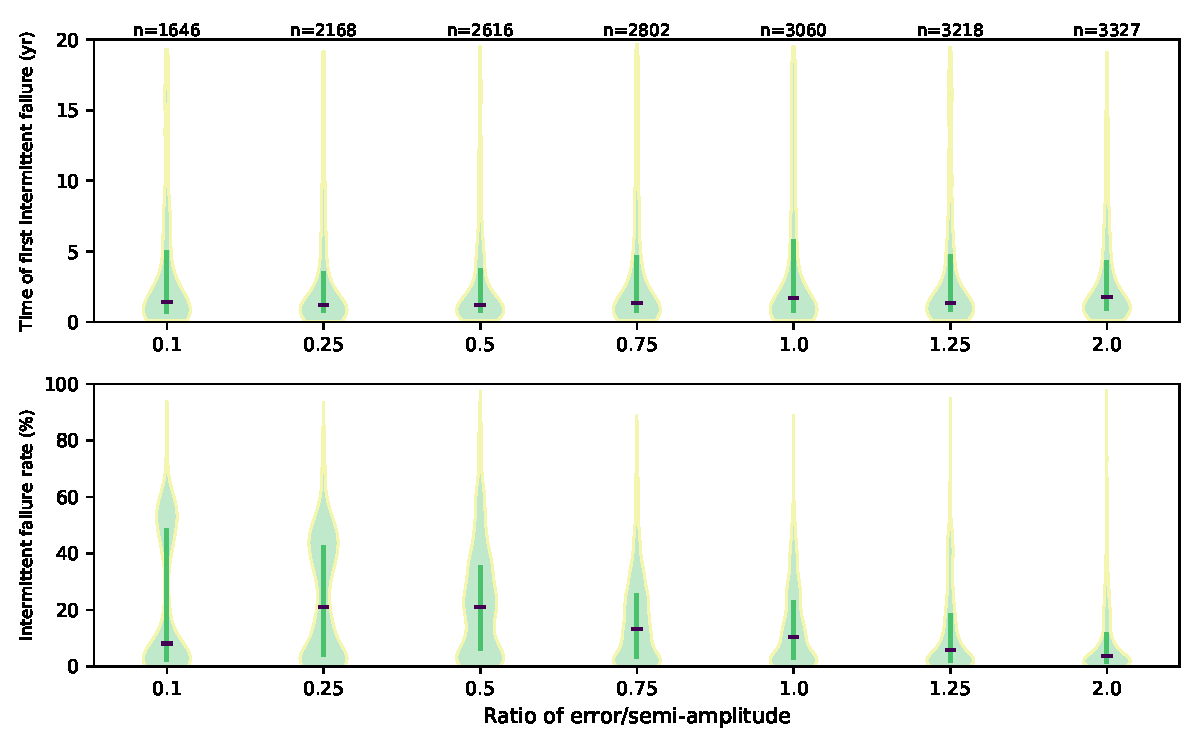
\includegraphics[width=\linewidth]{ch1/figures/violin_plots.pdf}
    \caption{Violin plots showing the variation of intermittent failure based on the ratio of RV
        error to RV semi-amplitude for the multivariate Gaussian method. Each violin shows the
        median (the horizontal black bar), the quartiles (the vertical green bars), and the kernel
        density estimate (the green curve to the left and right). The number of data points used for
        each ratio is labeled above the upper plot. We see that the distribution of the time of the
        first intermittent failure is weighted heavily near the start of the simulation with long
        tails for all ratios.  The intermittent failure rate is the number of intermittent failures
        divided by the number of times when the planet is not detectable. It is more variable, with
        low ratios having their distributions skewed to higher failure rates.  This is due to the
        dense clustering of orbits for low ratios, causing large failure rates when there is a
        period offset from the true planet.}%
    \label{fig:violin}
\end{figure}

To quantify how the ratio of RV error to RV semi-amplitude affects the scheduling of direct
imaging observations we fixed the semi-amplitude at 1 m/s and varied the RV error. We tested 
1$\sigma$ errors on RV measurements of 0.1, 0.25, 0.5, 0.75, 1, 1.25, and 2 m/s.  To generate true
planets we fixed $e$ at 0, $\omega$ at 0, $p$ at 0.367, mean anomaly at the initial time of RV
observation at 0, the star's mass at 1 solar mass, and set the star's distance to 10 parsecs. To
introduce variability we sampled 250 inclinations between 90 and 170 degrees based on a sinusoidal
distribution and generated 2500 planets by applying those inclinations to 10 linearly spaced $a$
values between 1 and 2 AU. To fix the semi-amplitude $K$ at 1 m/s we use equation~\ref{eq:K} to
calculate $M_p$ to match the fixed parameters. 

For each planet, consistent orbits were constructed with the four methods discussed in
Section~\ref{sec:orbit_methods}, each constructed set of orbits was propagated for 20 years, and
the failure modes were calculated. To determine detectability we used HabEx's starshade parameters
given in the HabEx report \citep{gaudiHabitableExoplanetObservatory2020}: an inner working angle of 0.058 arcseconds, outer
working angle of $6$ arcseconds, and $\Delta\mathrm{mag}_0$ of 26.5.

The primary results are shown in Figure~\ref{fig:con_method_bar_comparison}. It demonstrates the
differences in the construction methods' performance for different ratios of RV error to RV
semi-amplitude. A very important caveat to Figure~\ref{fig:con_method_bar_comparison} is that any
construction method that produces a probability of detection curve that never disperses to the point
where its local probability of detection maxima and minima are within 0.05 of each other will have
no failures in scenarios when the planet is always visible. This occurs because intermittent failure
is meant to identify when using a probability of detection curve might result in a null detection,
which is never the case when a planet is always visible. It may seem like the max KDE and max
likelihood perform well, but nearly all of their success is from always detectable scenarios where
an arbitrary step function would show no failure as well. However, we cannot simply exclude the
scenarios when the planet is always detectable because those scenarios may also result in dispersion
failure. Because of that, the most important part of the figure is the ``No failure (not always
detectable)'' percentage which indicates success in scenarios where an observation has a chance to
fail. Unsurprisingly, the general trend is that as the ratio increases the constructed orbits fail
more frequently.  More importantly, Figure~\ref{fig:con_method_bar_comparison} shows the differences
in failure mode for the different construction methods.  

Multivariate Gaussian shows very few dispersion failures compared to credible interval, but it has
more constructed orbit populations with intermittent failures than credible interval does.
Figure~\ref{fig:con_method_bar_comparison} shows that the methods relying on a single set of fitting
parameters, max likelihood and max KDE, should seldom be trusted as they have very high
failure rates when the planet has periods of undetectability, even for low ratios. At the lowest
ratios, 0.1 and 0.25, the most conservative construction, credible interval, outperforms
multivariate Gaussian by $\sim 3 \%$ (summing the two ``no failure'' metrics together).  At a
ratio of 0.5 multivariate Gaussian performs $\sim 20 \%$ better than credible interval. At ratios of
0.75 and 1 multivariate Gaussian outperforms credible interval by $\sim 60 \%$. At a ratio of 1.25,
the only method that performs better than an arbitrary step function would is multivariate Gaussian
which is $\sim 5 \%$ above the max likelihood and max KDE values. For a ratio of 2, credible
interval and multivariate Gaussian both underperform max likelihood and max KDE, which (at such a
high ratio) are essentially arbitrary functions showing the percentage of planets that will always
be visible.

Due to the heavy computation requirements, the sample size was limited for
Figure~\ref{fig:con_method_bar_comparison}. We ran a longer simulation shown in
Figure~\ref{fig:bar_plot} to check if the smaller sample size was representative and found that the
percentages align very closely with Figure~\ref{fig:con_method_bar_comparison}. The largest
difference in the percentages was 1.38\% and the median difference was 0.35\%.

Separating the orbits into those that have intermittent failure and those that don't have intermittent failure does not tell
the complete story since a constructed orbit population can have many intermittent failures or a
single intermittent failure.  To differentiate the constructed orbit populations within a single
construction method, we investigated the multivariate Gaussian construction method as it has
variability that max likelihood and max KDE don't and has more intermittent failures for low ratios
than credible interval.  We calculated how long it took for the first intermittent failure to
occur, and defined the intermittent failure rate as the ratio of the number of intermittent failures
to the total number of time steps where the true planet is not detectable. The violin plots of
Figure~\ref{fig:violin} show those metrics broken up by ratio.  Note that each ratio has a different
number of data points since lower ratios had fewer constructed orbit populations with intermittent
failures. The median time of the first intermittent failure is within 2 years for all ratios which
suggests that if a constructed orbit population is going to fail it is likely to fail relatively
quickly. 

The intermittent failure rate plot shows that all medians are below 20\% but the lower ratios have
much different kernel density estimates than the higher ratios. The most obvious example is the
lowest ratio (0.10), which has a bimodal density estimate with a peak around 50\%. The constructed
orbit populations that result in those higher failure rates are very tightly clustered (in the
$\alpha$ vs $\Delta \textrm{mag}$ space) but have the true planet in a low density region, causing
them to have a high probability of detection at times when the true plant is not visible. As the ratio
increases the constructed orbit populations become less tightly clustered which makes the
constructed orbits less likely to have high intermittent failure rates because they are more likely
to have dispersion failure, which is not counted in the intermittent failure rate, and less likely
to peak quickly which makes them spend less time above the 90\% threshold (described in
Section~\ref{sub:intermittent_failure}).  This creates a
fundamental trade-off between intermittent failure and dispersion failure. An orbit construction
method with less clustering shows less intermittent failure but more dispersion failure.

\section{Conclusions}%
\label{sec:conclusions}
We have presented and analyzed four methods for constructing orbit populations for use in direct imaging
from the information given by a radial velocity fit.  We further defined and analyzed two metrics that
indicate whether a constructed orbit population has failed for scheduling direct imaging observations. The first
failure mode, intermittent failure, represents times when the constructed orbits give false confidence
that a detection will be made. The second failure mode, dispersion failure, indicates that the
constructed orbits no longer provide information about when a planet will be detectable, and provides a 
clear definition for the problem of an orbit fit going ``stale''. Having those definitions in place
allows us to quantify how long an RV orbit fit can be used for direct imaging and the risks associated
with continuing to use it many years after the last radial velocity measurement.

To generalize our results we have looked at the ratio of 1 $\sigma $ error on RV measurements to the
RV semi-amplitude $K$ and showed quantitatively how decreasing that ratio increases the chance  of a
successful direct imaging observation. The results show a trade-off between the orbit construction
methods designed to cluster in high density regions of the $\alpha$ vs $\Delta \textrm{mag}$ space,
which risk failed observations when the true planet is in a low density region, and construction
methods that don't cluster as much, which disperse such that they don't give clear information on
when a detection is probable.

The major takeaways are that consistent orbit population construction methods based on a single set
of fitting basis parameters, as in the max likelihood or max KDE methods, perform poorly for direct
imaging scheduling.  For low ratios (0.1 and 0.25) of RV error to RV semi-amplitude the credible interval orbit
population construction method had the fewest failures.  The multivariate Gaussian orbit population
construction method had the fewest failures for ratios of RV error to RV semi-amplitude at 0.5 and
above.  There is an inherent trade-off between dispersion failure and intermittent failure, and more
conservative approaches (credible interval) have more dispersion failure.  Finally, if an orbit
population is going to have an intermittent failure, it is overwhelmingly likely to have its first
intermittent failure within a few orbital periods of when the fit is created.

Future work on this problem will involve optimizing the numerical values used to determine
intermittent failure for a specific mission and generalizing the multivariate Gaussian construction
method to improve its performance for low ratios of RV error to RV semi-amplitude. In this work, only
the top 1000 fitting basis parameter sets were taken to create the covariance matrix.  Increasing
that number will weight the high likelihood regions of the fitting basis space less, making the
constructed orbit population less dense (like the credible interval construction method) and perform
better for low ratios without ignoring correlations between the fitting basis parameters.  Having a
single orbit construction method that can be tuned for different ratios will provide a powerful tool
for mission planners for creating a direct imaging observation schedule. To verify that we will
implement this work into a direct imaging mission simulator.

% \section{Acknowledgments}
% This work was funded by the Science Investigation Team of the Nancy Grace Roman Space Telescope
% under NASA Grant NNX15AB40G.



\chapter{Coupling of Planet and Background Signal}
\label{cha:coupling}
\section{Introduction}%
\label{sec:ch2_intro}

Completeness as a metric has traditionally been defined under the assumption
that the photometric constraint is a flat, limiting $\Delta\textrm{mag}$ called
$\Delta\textrm{mag}_0$ \citep{brownSingleVisitPhotometric2005}, an assumption
that was used in \Cref{cha:first_paper}. This allows for fast computation of
completeness and therefore the impact of different $\Delta\textrm{mag}_0$
values on mission yield can be assessed quickly. However, when a mission's optical
system model is more established we can calculate $\Delta\textrm{mag}_0$ for
different observing scenarios, a specific combination of target, instrument,
and integration time. With more accurate $\Delta\textrm{mag}_0$ values we get a
more accurate photometric constraint and an improved value of completeness.
Ultimately, this can be used to determine which targets are worth extra
integration time.

Many factors ultimately play a role in the $\Delta\textrm{mag}_0$ for different
observing scenarios. A number of papers have described the impact of
integration time on completeness by assuming a constant $\Delta\textrm{mag}_0$
for a given integration time.\citep{hunyadiSingleVisitCompleteness2005,
brownNewCompletenessMethods2010, starkMaximizingExoEarthCandidate2014,
keithlyOptimalScheduling2020}. The $\Delta\textrm{mag}_0$ values have been
found by defining an equation for required integration time to reach a desired
signal-to-noise ratio (SNR) and inverting that equation to isolate the
$\Delta\textrm{mag}$ as a function of the integration time.
\citet{keithlyOptimalScheduling2020}, which analyzed an optical system based on
the Roman Space Telescope's coronagraph instrument \citep{Nemati2014}, used the
integration time equation,
\begin{equation}
  t = \frac{\textrm{SNR}^2 r_n}{r^2_\textrm{pl} - \textrm{SNR}^2 r^2_{\Delta I}}
  \label{eq:2020t}
\end{equation}
which has been used for a number of exoplanet direct imaging studies
\citep{nematiSensitivityWFIRST2017, delacroixScienceYield2016,
savranskyMultimissionModeling2017}, and expanded the planet count rate term,
$r_\textrm{pl}$, in terms of $\Delta\textrm{mag}$ to find the 
equation
\begin{equation}
  \Delta\textrm{mag}_i(t_{\textrm{int},i}) = -2.5 \log_{10} \frac{\textrm{SNR} \sqrt{\frac{r_{n,i}
    }{t_i} + r^2_{\Delta I, i} }}{C_{\mathcal{F}_0} 10^{-0.4 \nu_i (\lambda)}
T(\lambda, \alpha) \epsilon_{\textrm{PC}}}
  \label{eq:dean_dmag}
\end{equation}
where $t_{\textrm{int},i}$ is the integration time of the $i$'th target,
$r_{n,i}$ is the random variance count rate (or background noise count rate),
$r_{\Delta I,i}$ is the residual speckle count rate (the count rate of speckle noise after post processing effects),
$C_{\mathcal{F}_0}$ is the spectral flux density,
$\lambda$ is the observing wavelength,
$\nu_i$ is the target star's apparent magnitude,
$\alpha$ is angular separation between the planet and its star,
$T$ is the instrument's core throughput (the fraction of the planet's light collected by
the primary that ends up inside the area circumscribed by the half-max contour
of the planet's PSF \citep{Nemati2020a}), and $\epsilon_{\textrm{PC}}$ is the
photon-counting efficiency of the system.

\citet{keithlyOptimalScheduling2020} notes that $T$ is a function of $\alpha$,
but that without assuming a constant $\alpha$ the calculation of completeness
becomes much slower, as the limiting $\Delta\textrm{mag}$ becomes a function of
$\alpha$, and that the completeness values may be inaccurate for instruments
where core throughput changes considerably with $\alpha$. In this work, we
describe how to calculate the $\Delta\textrm{mag}_0$ when the
$r_{n}$ term is coupled to the planet count rate $r_{\textrm{pl}}$.
In \Cref{sec:Coupling of background and planet signal} we describe a problem
that arises from an optical system model where the planet signal and the
background signal are coupled, then in \Cref{sec:numerically_inverting_ETC} we
show a numerical method for solving the signal coupling problem. In
\Cref{sec:coupling_results} we describe how to use the numerical method to
calculate accurate completeness values for known planets for the various Roman
Space Telescope's coronagraph instrument (Roman CGI) observing scenarios.
Ultimately we show the ten highest completeness planets for the Roman CGI.

\section{Coupling of background and planet signal} % (fold)
\label{sec:Coupling of background and planet signal}

The optical system laid out in \citet{keithlyOptimalScheduling2020} to create
\Cref{eq:dean_dmag}, based on the work of Bijan Nemati for the Roman CGI
\citep{Nemati2014, nematiSensitivityWFIRST2017, Nemati2020a}, works on the
assumption that the noise sources included in $r_{n}$ have no
dependence on the planet's $\Delta\textrm{mag}$. However, in newer formulations
of the Roman CGI exposure time calculator (ETC), there is such a dependence. Every
frame results in readout and clock-induced charge noise, and a brighter signal
will require a shorter exposure time per frame, resulting in more total frames
and therefore more total readout and clock-induced charge noise. The newer form
of the ETC is implemented in the \code{EXOSIMS} package's \code{Nemati\_2019}
module \citep{savranskyWFIRSTAFTACoronagraphScience2015} which is an adaptation
of the Roman CGI team's internal ETC.

\begin{figure}
  \begin{center}
    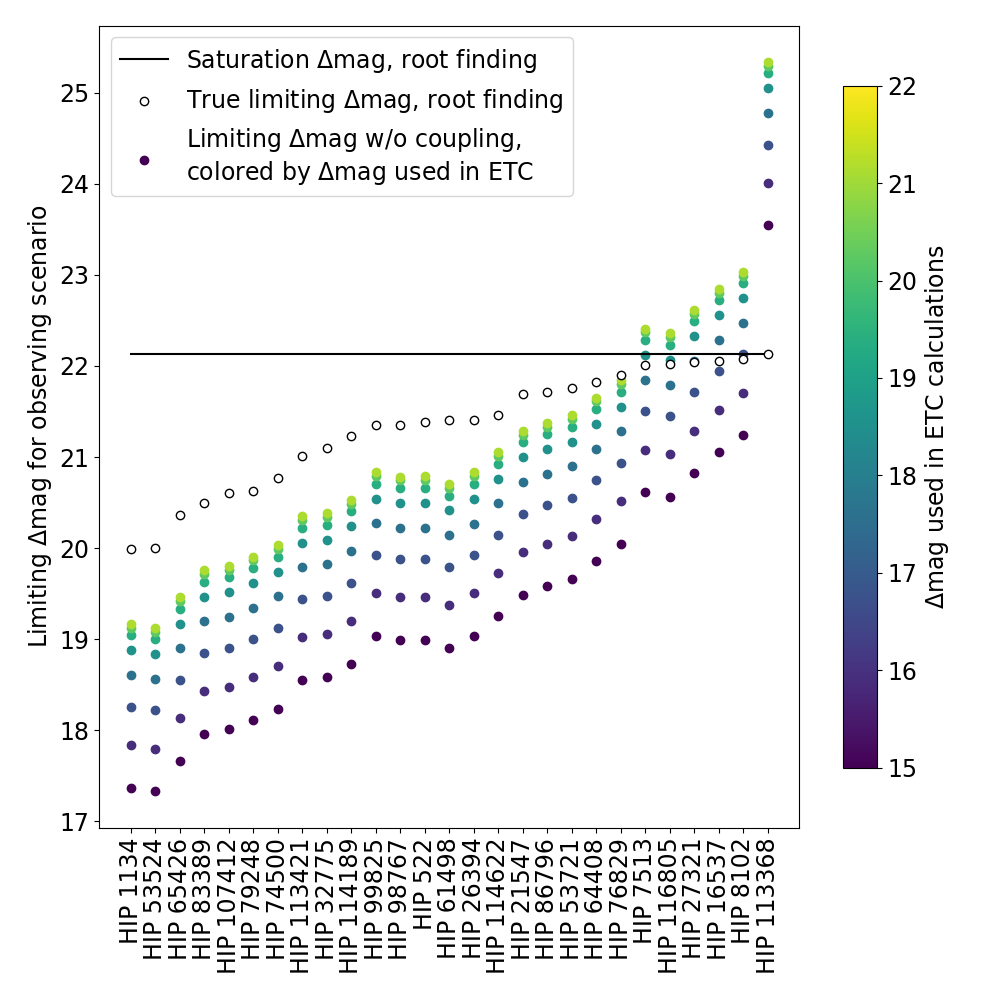
\includegraphics[width=0.95\textwidth]{ch2/figures/coupling.png}
  \end{center}
  \caption{Demonstrating the errors in limiting $\Delta\textrm{mag}$, the
  photometric constraint for completeness, when not treating the coupling
  between the planet signal and the noise factors. The observing scenario
  used for this plot is one day of integration time, the ``OPTI\_NF\_Imager''
  observing mode from the Roman CGI ETC, the target planet is fixed to an
  angular separation of $0.2955$ arcsec, zodiacal light surface brightness is fixed to
  $23 (\textrm{mag}/\textrm{arcsec})^2$, and exozodiacal light surface brightness is
  fixed to $22 (\textrm{mag}/\textrm{arcsec})^2$. The target stars included are the defaults
  in the Roman CGI ETC.}
  \label{fig:CGI_coupling}
\end{figure}

\begin{figure}
  \begin{center}
    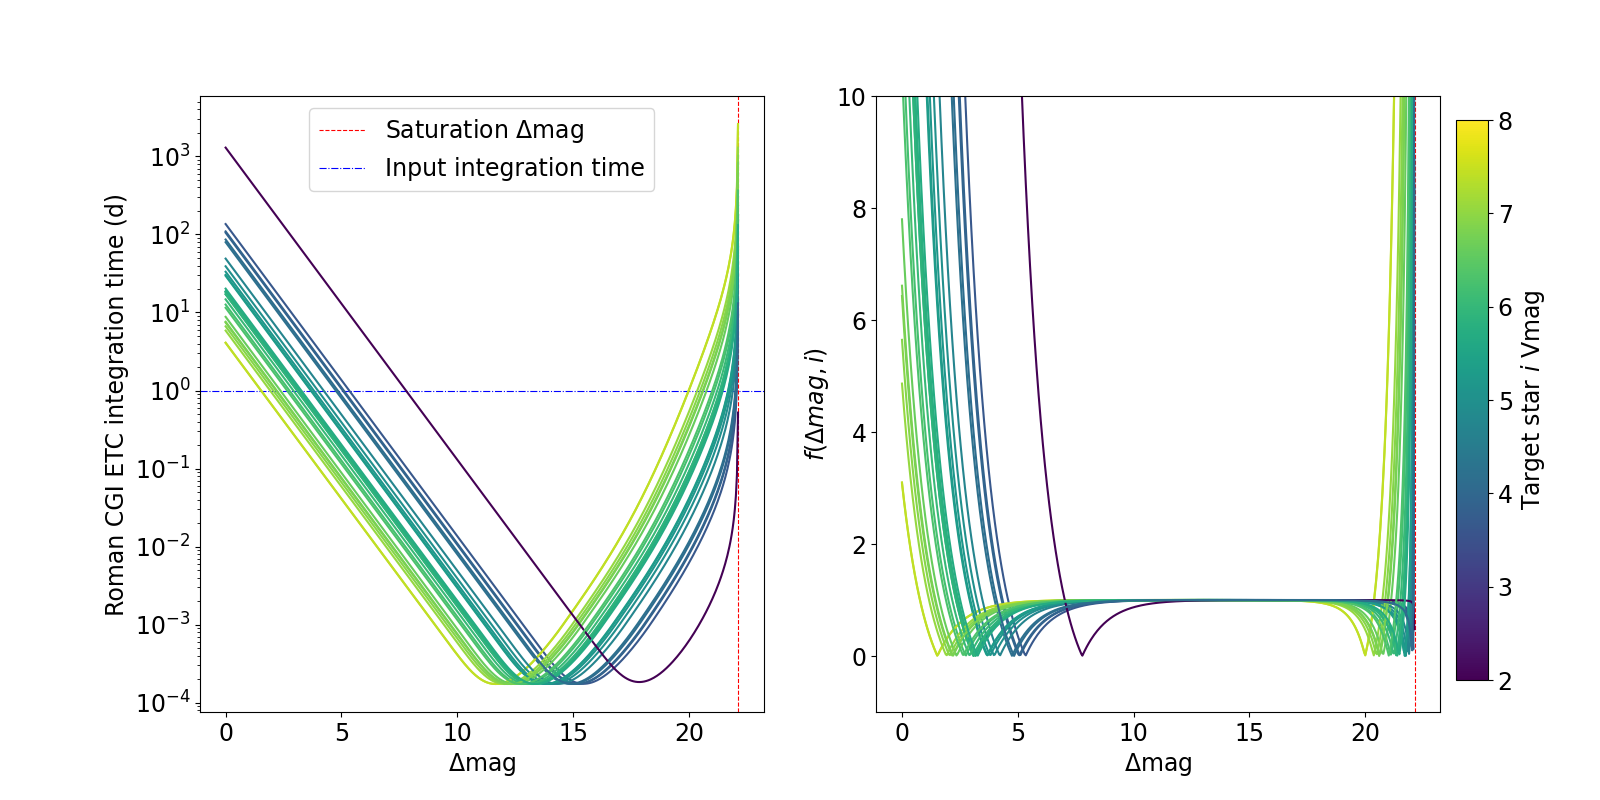
\includegraphics[width=0.95\textwidth]{ch2/figures/ETC_dMag_function.png}
  \end{center}
  \caption{Showing the Roman CGI's ETC integration time response to varying
  $\Delta\textrm{mag}$. Astrophysical inputs here are the same
  as in \Cref{fig:CGI_coupling}.}
  \label{fig:ETC_dMag_function}
\end{figure}

% \section{Coupling rewrite} % (fold)
% \label{sec:Coupling rewrite}
% STANDARDIZE TO ALL OF NEMATI 2020
The equation of signal-to-noise to noise ratio for the Roman CGI is modeled as
\begin{equation}
  \textrm{SNR} = \frac{r_\textrm{pl}t}{\sqrt{r_n t + r^2_{\Delta I} t^2}}
  \label{eq:2020SNR}
\end{equation}
% where SNR is the signal-to-noise ratio, $r_\textrm{pl}$ is the planet count
% rate, $t$ is the integration time, $r_n$ is the random variance count rate
% (background), and $r_{\Delta I}$ is the residual speckle rate, or the count
% rate of speckle noise after post processing effects. 
To calculate an exposure time for a specific SNR, planet, and star we can keep
the SNR, $r_\textrm{pl}$, $r_n$, and $r_{\Delta I}$ values constant and solve
for $t$ to get \Cref{eq:2020t}.
% \begin{equation}
%   t = \frac{\textrm{SNR}^2 r_n}{r^2_\textrm{pl} - \textrm{SNR}^2 r^2_{\Delta I}}.
%   \label{eq:2020t}
% \end{equation}
In a similar manner to calculating the
exposure time, the limiting $r_\textrm{pl}$ has traditionally been calculated
by solving \Cref{eq:2020SNR} as
\begin{equation}
  r_\textrm{pl} = \frac{\textrm{SNR} \sqrt{r_n t + r^2_{\Delta I} t^2}}{t}
  \label{eq:2020rpl}
\end{equation}
which is a useful quantity because it is the lowest planet count rate that meets
the required SNR. If we can isolate $r_\textrm{pl}$ then we can calculate a
$\Delta\textrm{mag}$ because
\begin{equation}
  r_\textrm{pl} = F_\lambda \Delta \lambda 10^{-0.4 \Delta \textrm{mag}} A \tau_\textrm{pl} \eta
  \label{eq:2020rpl_expand}
\end{equation}
where $F_\lambda$ is the spectral flux, $\Delta \lambda$ is the filter
bandwidth, $A$ is the collecting area, $\tau_\textrm{pl}$ is the throughput for
the planet light, and $\eta$ is the detector quantum efficiency. If we have a
specific $r_\textrm{pl}$ that represents the lowest possible value that reaches
the required SNR, then solving \Cref{eq:2020rpl_expand} for
$\Delta\textrm{mag}$ represents $\Delta\textrm{mag}_0$.

The trouble arises from the fact that in the newer formulation of the optical
system the $r_n$ term is now dependent on $r_\textrm{pl}$ in a significant
fashion. The equation is
\begin{equation}
  r_n = r_\textrm{pl} + k_\textrm{sp} r_\textrm{sp} + k_\textrm{lz}
  r_\textrm{lz}+ k_\textrm{ez} r_\textrm{ez}+ k_\textrm{det} r_\textrm{det}.
  \label{eq:rn}
\end{equation}
In \Cref{eq:rn} $r_\textrm{sp}$ is the speckle count rate, $r_\textrm{lz}$ is the count
rate of local zodiacal light, $r_\textrm{ez}$ is the count rate of
exozodical light, $r_\textrm{det}$ is the count rate of detector noise, and the
$k_x$ terms are variance enhancement factors for each count rate to account for
the effects of reference differential imaging. This has a clear dependence on
$r_\textrm{pl}$ but it has a further dependence through the $r_\textrm{det}$ term
in
\begin{equation}
  r_\textrm{det} =  m_\textrm{pix}\left( i_d +
  \frac{q_\textrm{CIC}}{t_\textrm{fr}} +
\frac{\sigma^2_\textrm{rd}}{t_\textrm{fr} G_\textrm{EM}} \right)
  \label{eq:rdet}
\end{equation}
where $i_d$ is the detector dark current, $m_{\textrm{pix}}$ is the number of
detector pixels that the planet signal covers, $q_{\textrm{CIC}}$ is the CCD
clock-induced charge, $t_{\textrm{fr}}$ is the frame duration,
$\sigma_{\textrm{rd}}$ is read noise, and $G_{\textrm{EM}}$ is the electron
multiplication gain. $\sigma_{\textrm{det}}^2$ is one of the four random noise
components for the target star in $C_{\textrm{b},i}$ (see \citet{Nemati2020a}
for more details). The $1/t_{\textrm{fr}}$ terms in
\Cref{eq:rdet} represent that the $q_\textrm{CIC}$
and $\sigma_\textrm{rd}$ terms are dependent on how many frames are taken over
the course of an observation. The equation for $t_\textrm{fr}$ is 
\begin{equation}
  t_{\textrm{fr}} = \frac{0.1}{DC +\left(r_{\textrm{pl}}+r_{\textrm{lz}}+r_{\textrm{ez}}+r_{\textrm{sp}}\right)/m_{\textrm{pix}}}
  \label{eq:bijan_frame_duration}
\end{equation}
where $DC$ is the detector dark current noise per second.
\Cref{eq:bijan_frame_duration} comes from the Roman CGI team and is restricted
to be between 1 and 80 seconds (personal communication, Oct 5, 2022).

To complicate the relationship further, the $t_{\textrm{fr}}$ value impacts the
number of cosmic ray hits per frame and the charge transfer efficiency. Those
end up impacting the detector degradation which then impacts all count
rates. 
By making $r_n$ a complex function of $r_\textrm{pl}$ we are unable to isolate
it as a function of SNR, $r_n$, $r_{\Delta I}$, and $t$ analytically. Therefore
to calculate the $\Delta\textrm{mag}_0$ for a specific observing scenario we
need to invert the relationship numerically.

\Cref{fig:CGI_coupling} shows the errors that occur when trying to
calculate the $\Delta\textrm{mag}_0$ values without accounting for the rate
coupling. The colored circles represent calculating $\Delta\textrm{mag}$
from \Cref{eq:2020rpl,eq:2020rpl_expand} and using a constant
$\Delta\textrm{mag}$ value for the $r_n$ term. The true $\Delta\textrm{mag}$
values, the empty circles, deviate significantly and in many cases would result
in underestimating $\Delta\textrm{mag}_0$. The direction of the error is driven
by how close the $\Delta\textrm{mag}_0$ is to the saturation
$\Delta\textrm{mag}$, or the $\Delta\textrm{mag}$ at which $\left(\textrm{SNR}
\cdot r_{\Delta I}\right)^2$ becomes greater than $r_{\textrm{pl}}$ in
\Cref{eq:2020t} and the calculated integration times become
negative.

% section sec:Coupling rewrite (end)


\section{Numerically Inverting the Roman CGI Exposure Time Calculator}
\label{sec:numerically_inverting_ETC}

To restate the problem, we want to determine the completeness for a given
integration time, $t_{\textrm{int}}$. The photometric constraint in the
completeness calculation is defined as the dimmest planet that meets the
required SNR. However, the brightness of that planet affects both the signal
and the noise. Failing to account for the changes in the noise term can lead to
overly optimistic photometric constraints, systematically over estimating
completeness. By inputting different $\Delta\textrm{mag}$ values in the
ETC, with the SNR fixed to the required value, we can
determine which $\Delta\textrm{mag}$ results in the integration time
$t_{\textrm{int}}$ that we are trying to calculate completeness for.

Repeatedly running the ETC is computationally costly so we formulate it as a
minimization problem to reduce the number of evaluations necessary. The
objective function for this minimization is
\begin{equation}
  f(\Delta\textrm{mag}, i) = |t_{\textrm{int}} -
  t_{\textrm{ETC}}(\Delta\textrm{mag}, \textrm{SNR}, i)|
  \label{eq:intTime_root_obj}
\end{equation}
where $t_{\textrm{ETC}}$ is a call to our ETC for target star $i$ for a
specific observing scenario. The minimization is complicated by the fact that
$f\left(\Delta\textrm{mag}, i\right)$ has two minima, as shown on the right plot of
\Cref{fig:ETC_dMag_function}. As we are looking for
$\Delta\textrm{mag}_0$, our goal is to converge to the larger of the local
$\Delta\textrm{mag}$ minima. The lower of the minima is caused by the model for
$C_b$ increasing exponentially as $\Delta\textrm{mag}$ goes to zero. The target
star's V magnitude affects the location where the slope changes, which can be
seen in \Cref{fig:ETC_dMag_function} where the line colors represent the V
magnitude.

The ETC also has a saturation value, $\Delta\textrm{mag}_\textrm{sat}$. At
$\Delta\textrm{mag}_\textrm{sat}$ the integration time goes to infinity,
representing the $\Delta\textrm{mag}$ where even an infinite integration time
would be insufficient to detect a planet of that $\Delta\textrm{mag}$. Any
$\Delta\textrm{mag}$ value greater than $\Delta\textrm{mag}_\textrm{sat}$ also
will never be detected. $\Delta\textrm{mag}_\textrm{sat}$ is marked as an
asymptote in \Cref{fig:ETC_dMag_function}. Because of this we will use the
$\Delta\textrm{mag}_\textrm{sat}$ as the upper bound for our minimization,
$\Delta\textrm{mag}_{ub}$. The $\Delta\textrm{mag}_{ub}$ can be found by
running root finding on 
\begin{equation}
  C_{\textrm{p}} - \left(\textrm{SNR} \cdot C_{\textrm{sp}}\right)^2
  \label{eq:sat_root}
\end{equation}
for different values of $\Delta\textrm{mag}$.

The lower bound should be set such that the domain of $f\left(\Delta\textrm{mag},
i\right)$ is limited to the $\Delta\textrm{mag}$ values where the integration
times are strictly increasing so that the minimization doesn't converge to the
lower bound because it is approaching the lower $\Delta\textrm{mag}$ minima. As
a heuristic, we begin with
\begin{equation}
  \Delta\textrm{mag}_{lb}(i) = \Delta\textrm{mag}_{ub}(i) - 2 - V(i)
  \label{eq:dMag_lb}
\end{equation}
which resulted in convergence for the minimization in over 99\% of cases for
the Roman CGI's narrow field of view imaging instrument. The routine is implemented
as the \code{calc\_dMag\_per\_intTime} function in the \code{Nemati}
module in the \code{EXOSIMS} package. The minimization function itself
is \code{SciPy}'s \citep{virtanenSciPyFundamental2020} implementation of the
bounded scalar minimization routine from \citet{forsytheComputerMethods1977}
with a tolerance of $10^{-8}$ on $f(\Delta\textrm{mag}, i)$. The function
requires as input the local and exozodiacal light surface brightnesses,
as they are required by the CGI's ETC. In this work, we use a local zodiacal
light surface brightness of $Z=23
\frac{\textrm{mag}}{\textrm{arcsec}^2}$ and exozodiacal light surface
brightness of $EZ=22 \frac{\textrm{mag}}{\textrm{arcsec}^2}$
taken from \citet{starkMaximizingExoEarthCandidate2014}. Some example
minimization calculations are shown in \Cref{fig:minimization_star_comp}.
\begin{figure}
  \begin{center}
    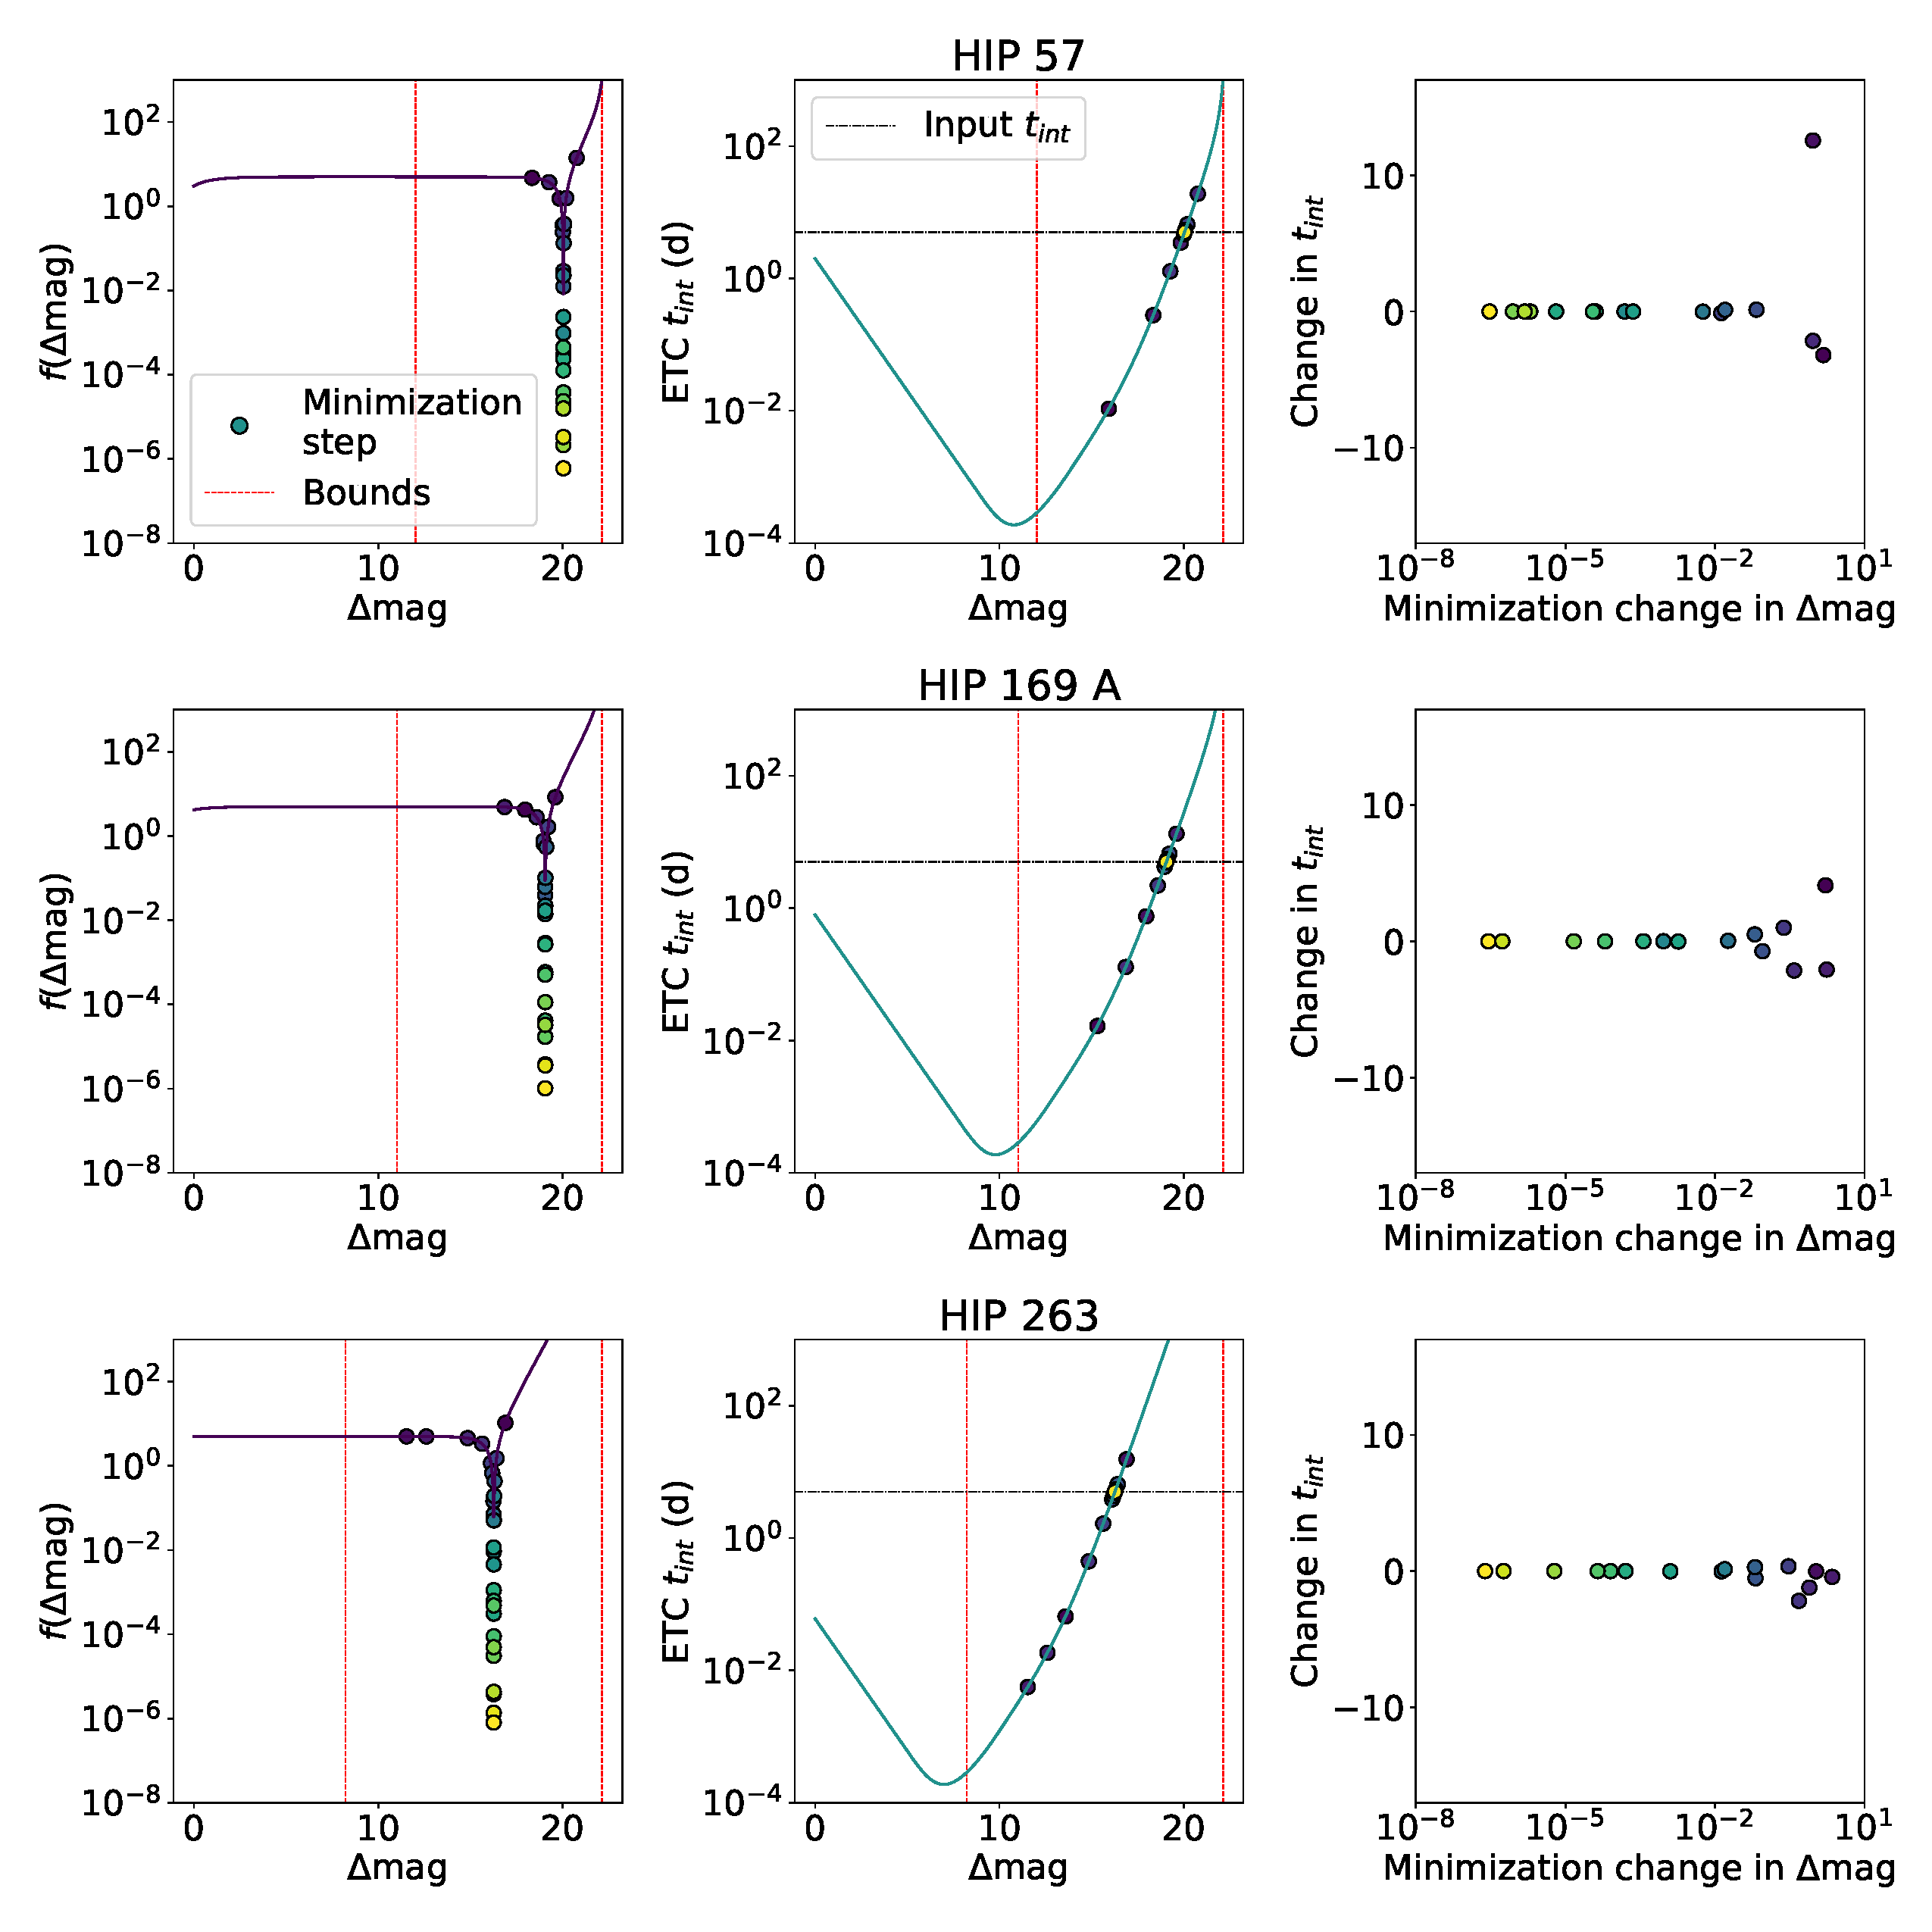
\includegraphics[width=0.95\textwidth]{ch2/figures/minimzation_star_comp.pdf}
  \end{center}
  \caption{Demonstrating successful inversion of the Roman CGI's ETC using the minimization
    routine on HIP 57, HIP 169 A, and HIP 263. Each dot represents a step the
  minimization routine took, with the first step in dark purple and the last in
bright yellow. Each row represents a specific star. The left column shows the
minimization steps compared to the minimization objective function,
\Cref{eq:intTime_root_obj}, and the $\Delta\textrm{mag}$ bounds given to the
minimization routine. The middle column shows the corresponding integration
times for the steps taken by the minimization routine, the $\Delta\textrm{mag}$
bounds, and the input $t_\textrm{int}$ that the minimization routine is
attempting to converge to. The right column shows the $\Delta\textrm{mag}$ step
sizes and their corresponding change in $t_\textrm{int}$.}
  \label{fig:minimization_star_comp}
\end{figure}

\begin{figure}
  \begin{center}
    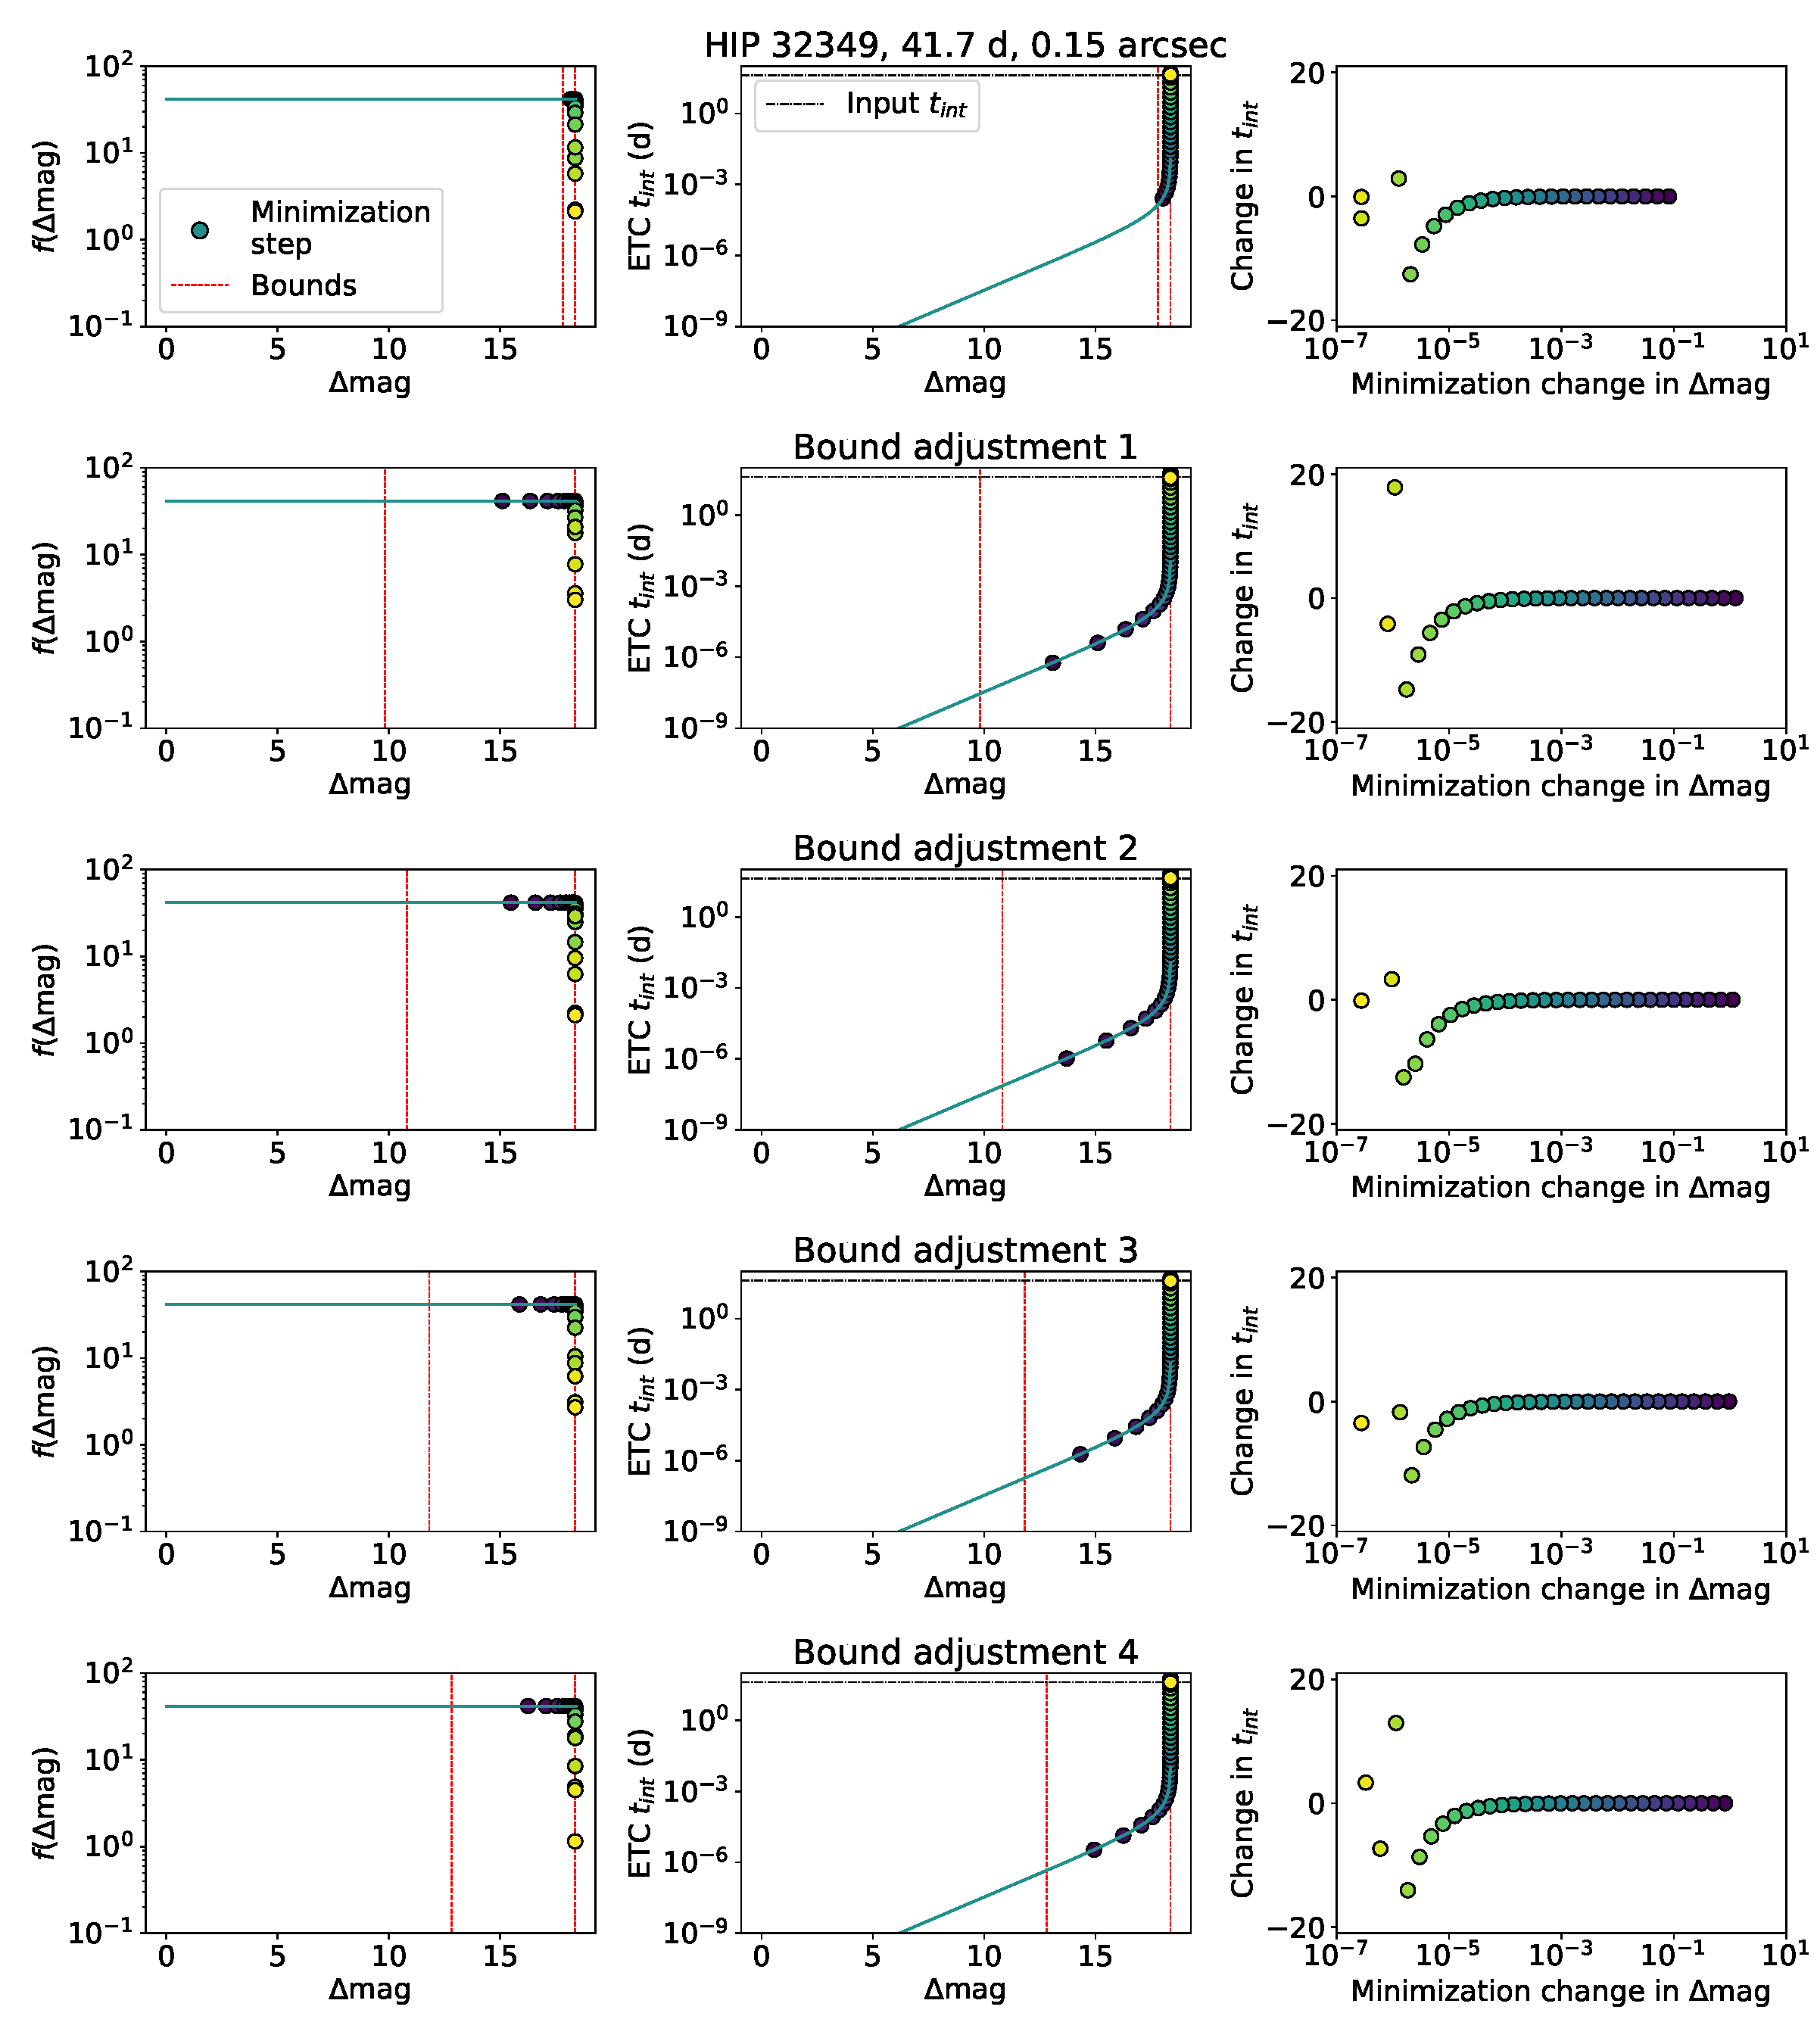
\includegraphics[height=0.75\textheight]{ch2/figures/minimzation_bound_comp.pdf}
  \end{center}
  \caption{The minimization process succeeding with an exceptionally difficult
    scenario, right on the inner working angle of Roman CGI's narrow field
    instrument with a long integration time requested. The progression of the
    lower bounds is shown from top to bottom. The algorithm ultimately finds a
  solution within the 5\% tolerance on the fifth minimization. Note the large
changes in integration time during the last steps which are on the order of
$10^{-6}$ $\Delta\textrm{mag}$.}
  \label{fig:minimzation_bound_comp}
\end{figure}

The two problems we can run into are converging to the lower bound and trying
to find the $\Delta\textrm{mag}$ for an integration time where the greater of the
minima is on the asymptote. In extreme cases the slope of $(\Delta  t_{\textrm{int}}) /
\left(\Delta(\Delta\textrm{mag})\right)$ can be too great for the minimization
routine to converge to the requested tolerance. To handle this we wrap the
minimization in a loop. If the minimization converges to the lower bound, the
lower bound is raised by one and the minimization is run again. If the
resulting lower bound is greater than the upper bound then \Cref{eq:dMag_lb} is
modified to subtract 10 instead of 2. For the case where the solution is on the
asymptote, we allow the routine to stop when the solution value is within 5\% of
the given integration time as the $\Delta\textrm{mag}$ error will be on the
order of $10^{-7}$. \Cref{fig:minimzation_bound_comp} demonstrates the worst
case scenario, where the solution was found after 5 minimization iterations,
found by running the root-finding method on 100 combinations of $t_\textrm{int}$ and
$\alpha$ for all of the stars in the EXOCAT target list
\citep{turnbullExoCat1Nearby2015} with all of the observing scenarios in the
Roman CGI ETC (\url{github.com/hsergi/Roman_Coronagraph_ETC}). If no solution
is found the function will raise an error and exit, indicating that under no
scenario will the exposure time calculator return the inputted integration time.

\begin{figure}
  \begin{center}
    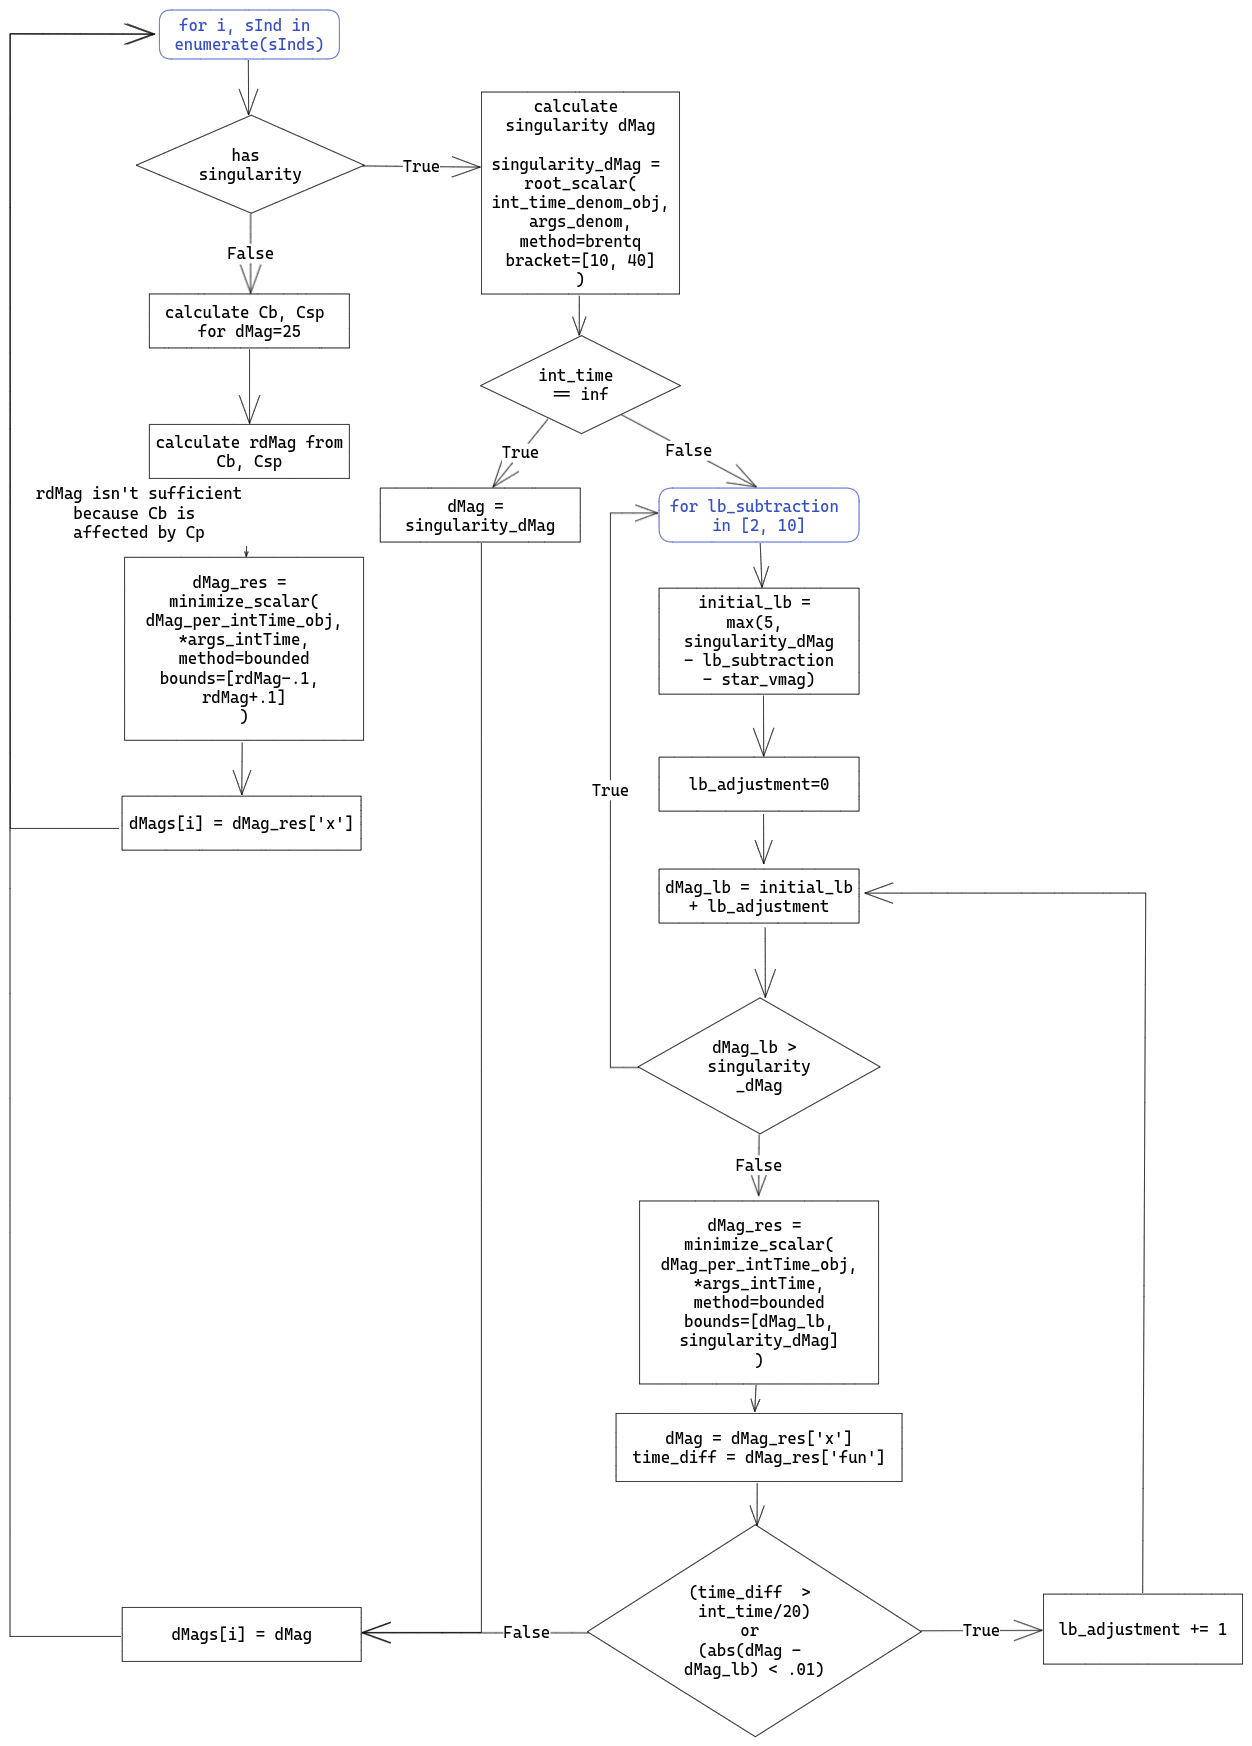
\includegraphics[width=0.95\textwidth]{ch2/figures/root_flowchart.png}
  \end{center}
  \caption{Process of calculating the dimmest detectable $\Delta\textrm{mag}$ given
  an integration time. Uses EXOSIMS naming scheme and Python syntax.}
  \label{fig:root_flowchart}
\end{figure}

The full numerical routine can be seen in \Cref{fig:root_flowchart}.
Effectively the routine turns the flat $\Delta\textrm{mag}_0$ into a function
$\Delta\textrm{mag}_0(t_\textrm{int}, \alpha)$ for the observing scenario of
interest. A major benefit of a numerical routine for solving this is its
robustness. As the optical system models evolve this numerical routine will not
need to be updated in the same fashion that an analytical formulation would.
Additionally, if a change is made to the optical system model and the impact
on an analytical equation for $\Delta\textrm{mag}_0$ is not immediately noticed
it can lead to systematic underestimates or overestimates of the required
observation time to reach a desired completeness.

\section{Results}%
\label{sec:coupling_results}

We worked with the Roman CGI team to establish the completeness of the planets
in NASA Exoplanet Archive \citep{akesonNASAExoplanet2013} for the Roman CGI's
various observing scenarios. The results can be seen in full at the Imaging Mission Database
(\url{plandb.sioslab.com}), a website that pulls all of the planets from the
Exoplanet Archive with sufficient orbital information to establish a density
function of possible $\Delta\textrm{mag}$ and $\alpha$ values as described in
\citet{savranskyExplorationDynamical2019}. The Roman CGI team created eighteen
observing scenarios of interest, three of the four observing modes for three
$t_\textrm{int}$ times each (``minimum'', ``medium'', and ``maximum''), with 2
different error budgets. The observing modes are narrow field imaging, wide
field imaging, and spectroscopy.

The narrow field imaging is achieved with the hybrid Lyot coronagraph with a
filter centered at 575 nm, wide field imaging is done with a shaped pupil
coronagraph (SPC) with a filter centered at 825 nm, and spectroscopy is done
with a separate SPC in a ``bowtie'' shape with a filter centered at 730 nm
\citep{kasdinNancyGrace2020}. 
% For a full description of the observing modes see \citet{kasdinNancyGrace2020},
% but here is a short description of each.
The imaging modes were considered at $t_\textrm{int}$ values of 25, 100, and
10000 hours while the spectroscopy mode was considered at $t_\textrm{int}$
values of 100, 400, and 10000 hours. These times were chosen to represent
short, medium, and infinite integration times. Finally, the observing modes had
both an ``Optimistic'' and ``Conservative'' error budget based on the model
uncertainty factors (MUF) established internally by the Roman CGI team. 
Individual observing scenarios are labeled as a combination of all of these
factors, e.g. ``Conservative NF Imager 25hr''.

\begin{figure}
  \begin{center}
    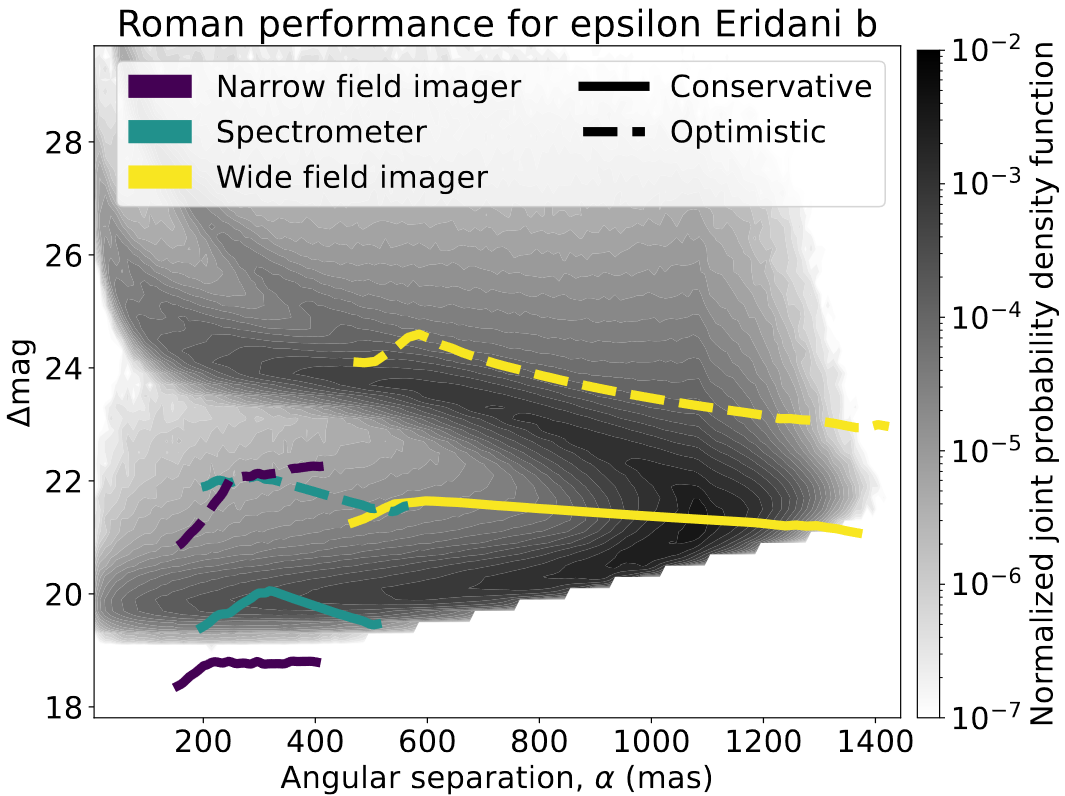
\includegraphics[width=0.95\textwidth]{ch2/figures/RST_performance_flipped.png}
  \end{center}
  \caption{The performance of the Nancy Grace Roman Space Telescope's coronagraph
    instruments when observing the planet epsilon Eridani b. ``Optimistic'' is the
  optimistic error budget with maximum integration time while ``Conservative''
  is the conservative error budget with minimum integration time.}
  \label{fig:RST_performance_flipped}
\end{figure}

For each observing scenario, the $t_\textrm{int}$ value is specified so our
$\Delta\textrm{mag}_0$ is strictly a function of $\alpha$, where $\alpha \in
[\textrm{IWA}, \textrm{OWA}]$ for the observing mode's IWA and OWA. By applying
the method described in \Cref{sec:numerically_inverting_ETC} we generated the
$\Delta\textrm{mag}_{0,i,j}(\alpha)$ values for every star $i$ in the
Imaging Mission Database for the 18 observing scenarios $j$. The joint density
functions $f_k(\Delta\textrm{mag}, \alpha)$ for each planet $k$ were already
calculated for the known planets, as described in
\citet{savranskyExplorationDynamical2019}. We can then calculate the
completeness for a planet $k$ around star $i$ with observing scenario $j$
\begin{equation}
  c_{j,k} = \int_{\textrm{IWA}_j}^{\textrm{OWA}_j}\int_0^{\Delta\textrm{mag}_{0,i,j}(\alpha)} 
  f_k (\Delta\textrm{mag}, \alpha)
  \textrm{d}\Delta\textrm{mag}\textrm{d}\alpha
  \label{eq:c_plandb}
\end{equation}
which allows us to estimate the sensitivity of the various observing scenarios
to known planets. This can be visualized by overlaying the
$\Delta\textrm{mag}_{0,i,j}(\alpha)$ lines on a joint density function
$f_k(\Delta\textrm{mag}, \alpha)$, as shown in
\Cref{fig:RST_performance_flipped}, and looking at the area under a given
$\Delta\textrm{mag}_{0,i,j}(\alpha)$ line. The completeness values for the
scenarios in \Cref{fig:RST_performance_flipped} are shown in
\Cref{tab:eps_eri_table}, demonstrating that wide field imaging mode has the highest
completeness for epsilon Eridani b. \Cref{tab:eps_eri_table} shows that for the narrow field
imager, increasing $t_\textrm{int}$ has almost no effect because the narrow field imager is effectively
at the saturation point at $t_\textrm{int}=25$ for epsilon Eridani. The wild field
imager is not at the saturation point at $t_\textrm{int}=25$ which results in a
difference of $\sim$0.077 $c$ between $t_\textrm{int}=25$ hr and
$t_\textrm{int}=100$ hr.

\begin{table}
  \caption{Completeness of epsilon Eridani b under the 18 different observing scenarios.}
  \label{tab:eps_eri_table}
  \begin{center}
    \begin{tabular}{|cccc|}\hline
      \bfseries Scenario &
      \bfseries Minimum $t_\textrm{int}$ &
      \bfseries Medium $t_\textrm{int}$ &
      \bfseries Maximum $t_\textrm{int}$
      \csvreader[head to column names]{ch2/figures/eps_eri.csv}{}
      {\\\hline\csvcoli\ & \csvcolii & \csvcoliii & \csvcoliv}
      \\\hline
    \end{tabular}
  \end{center}
\end{table}

This process was run on all planets in the Exoplanet Archive and the resulting
completeness values were incorporated into the Imaging Mission Database. The
ten highest completeness planets and the observing scenarios to maximize
completeness for the planets are shown in
\Cref{tab:top_comp_planets}.
\begin{table}
  \caption{Highest completeness planets on \url{plandb.sioslab.com} and their respective
  observing mode.}
  \label{tab:top_comp_planets}
  \begin{center}
    \begin{tabular}{|c|c|c|c|}\hline
      \bfseries Planet &\bfseries $c$ &\bfseries Observing scenario
      \csvreader[head to column names]{ch2/figures/plandb_data.csv}{}
      {\\\hline\csvcoli\ & \csvcolii & \csvcoliii}
      \\\hline
    \end{tabular}
  \end{center}
\end{table}

\section{Conclusion}

In this chapter, we have demonstrated that the current exposure time calculator
for the Roman Space Telescope's coronagraph instrument cannot be analytically inverted to
isolate $\Delta\textrm{mag}$ as a function of $t_\textrm{int}$ because the
background signal is a function of the $\Delta\textrm{mag}$ value. We have
demonstrated how to handle completeness calculations with that limitation by
inverting the ETC with a numerical minimization routine implemented in
\code{EXOSIMS}. With this routine, we can establish the photometric constraint
($\Delta\textrm{mag}_0$) for the calculation of completeness for any observing
scenario when there is a coupling between the planet and background signals. By
calculating the $\Delta\textrm{mag}_0$ value over a range of $\alpha$ values we
can account for the change in throughput at smaller separations and avoid
systematically overestimating the completeness values for planets at small
separations. We applied this process to create the Roman Space Telescope's
observing scenario completeness values for the Imaging Mission Database. By
using the Imaging Mission Database a researcher can see the sensitivity of the
various Roman CGI observing modes to different known planets.

% sec:Coupling of background and planet signal (end)

% This dependence is somewhat hidden, but it begins with equation 48 of \citet{Nemati2020a},
% \begin{equation}
%   \sigma_{\textrm{det}}^2 = i_d m_{\textrm{pix}} t + q_\textrm{CIC} m_{\textrm{pix}} \frac{t}{t_{\textrm{fr}}}
%   + m_{\textrm{pix}} \frac{t}{t_{\textrm{fr}}} \left( \frac{\sigma_{\textrm{rd}}}{G_{\textrm{EM}}}\right)^2
%  \label{eq:bijan_detector_noise}
% \end{equation}
% where $\sigma_{\textrm{det}}^2$ is the CCD detector noise variance, $i_d$ is
% the detector dark current, $m_{\textrm{pix}}$ is the number of detector pixels
% that the planet signal covers, $t_\textrm{int}$ is the integration time, $q_{\textrm{CIC}}$
% is the CCD clock-induced charge, $t_{\textrm{fr}}$ is the frame duration,
% $\sigma_{\textrm{rd}}$ is read noise, and $G_{\textrm{EM}}$ is the electron
% multiplication gain. $\sigma_{\textrm{det}}^2$ is one of the four random
% noise components for the target star in $C_{\textrm{b},i}$, see \citet{Nemati2020a} for more details.
% The $t_\textrm{int}/t_{\textrm{fr}}$ terms in equation~\ref{eq:bijan_detector_noise} are
% equal to the number of frames collected over the full integration time $t_\textrm{int}$,
% which is where the coupling between the planet and noise ultimately comes from.
% The way that the frame time calculation has been implemented in the Roman ETC
% is
% \begin{equation}
%   t_{\textrm{fr}} = \frac{0.1}{DC +\left(r_{\textrm{pl,ia}}+r_{\textrm{zo,ia}}+r_{\textrm{sp,ia}}\right)/m_{\textrm{pix}}}
%   \label{eq:bijan_frame_duration}
% \end{equation}
% where $DC$ is the detector dark current noise per second, $r_{\textrm{pl,ia}}$ is
% the planet electron count rate at the image area per pixel per second,
% $r_{\textrm{zo,ia}}$ is the zodiacal light electron count rate at the image area
% per pixel per second, $r_{\textrm{sp,ia}}$ is the speckle electron count rate at
% the image area per pixel per second, and is cut to be between 1 and 80 seconds. This
% is not in literature and was pulled from a private GitHub repository that hosts the
% ETC.

% The equation for $r_{\textrm{pl,ia}}$ is
% \begin{equation}
%   r_{\textrm{pl,ia}} = F_p f_{\textrm{SR}} A_{\textrm{col}} \textrm{QE} \tau_{\textrm{PS}}
%   \label{eq:bijan_planet_ia}
% \end{equation}
% where $F_p$ is the planet's flux, $f_{\textrm{SR}}$ is the fraction of light in
% the signal region, $A_{\textrm{col}}$ is the collecting area of the primary, QE
% is the quantum efficiency, and $\tau_{\textrm{PS}}$ is the throughput of a
% point source. By expressing the planet's flux in terms of the star's flux $F_s$
% and $\Delta\textrm{mag}$,
% \begin{equation}
%   F_p = F_s 10^{-\Delta\textrm{mag}/2.5},
%   \label{eq:fp_dmag}
% \end{equation}
% we see how the $\Delta\textrm{mag}$ term ends up in the calculation of
% $C_{\textrm{b}}$. If the $r_{\textrm{pl,ia}}$ term was removed from
% equation~\ref{eq:bijan_planet_ia} the coupling would be removed, but it is
% prudent to account for the planet's signal, especially for observing scenarios
% which consider bright planets.

% To complicate the relationship further, the $t_{\textrm{fr}}$ value impacts the
% number of cosmic ray hits per frame and the charge transfer efficiency. Those
% end up impacting the detector degradation (dQE) which then impacts the count
% rates for the planet, zodiacal light, and extra zodiacal light. This makes it
% impossible to invert the exposure time calculator and isolate
% $\Delta\textrm{mag}$ as a function of integration time analytically. Our approach,
% laid out in Section~\ref{sec:numerically_inverting_ETC} explains our numerical
% solution with root finding.

% Figure~\ref{fig:CGI_coupling} shows the errors that occur when trying to
% calculate the $\Delta\textrm{mag}_0$ values with equation~\ref{eq:dean_dmag},
% the colored circles. The true $\Delta\textrm{mag}$ values, the empty circles,
% deviate significantly and in many cases would result in underestimating
% $\Delta\textrm{mag}_0$. The direction of the error is driven by how close the
% $\Delta\textrm{mag}_0$ is to the saturation $\Delta\textrm{mag}$, or the
% $\Delta\textrm{mag}$ at which $\left(\textrm{SNR} \cdot C_{\textrm{sp}}\right)^2$ becomes greater than $C_{\textrm{p}}$ in
% equation~\ref{eq:dean_inttime} and the calculated integration times become
% negative.

% Further, the impact on completeness is incredibly difficult to characterize,
% since that the zodiacal light terms are involved.

% Figure~\ref{fig:dMag_error} shows the problem of trying to calculate
% $\Delta\textrm{mag}$ without accounting for the coupling. The ``Assumed $\Delta
% \textrm{mag}$'' refers to the user-inputted $\Delta \textrm{mag}$ that is used
% when calculating $C_{\textrm{b}, i}$. The highest assumed $\Delta \textrm{mag}$
% of 15 shows the worst performance, while the lowest assumed $\Delta
% \textrm{mag}$ of 25 has relatively small errors. This coupling is significant
% in many cases, and makes it impossible to analytically solve for
% $\Delta\textrm{mag}$ as a function of integration time. Therefore we must
% approach it as a numerical problem.


\chapter{Accurate Estimation of Probability of Imaging Detection with Precursor Radial Velocity Data}
\label{cha:accurate_pdet}
\section{Introduction}
\label{sec:accurate_pdet_intro}

As described in \Cref{cha:first_paper} future missions are expected to use
orbital information collected from radial velocity (RV) fits to create their
initial observation schedule. Directly imaging an Earth-like planet is very
dependent on the planet's position along its orbit because its orbital phase
determines the amount of light reflecting off the planet and the fact that at
smaller angular separation's $\alpha$ a telescope will collect less of the planet's
light. In \Cref{cha:first_paper} a method of creating orbits consistent
with the underlying radial velocity data was detailed and the probability
of detection was calculated as
\begin{equation}
    P_{\textrm{det}}(t) = \frac{\textrm{Number of orbits detectable at time $t$}}{\textrm{Number of
    constructed orbits}}
.\end{equation}
This equation is an accurate description of the probability of detection
$P_\textrm{det}$, however, the ``Number of orbits detectable at time $t$'' factor
was hiding a lot of complexity. The constraints used to establish whether an orbit
was detectable were
\begin{align}
    \text{IWA} < \alpha < \text{OWA}\\
    \Delta\mathrm{mag} < \Delta\mathrm{mag}_0
\end{align}
where the $\Delta\textrm{mag}_0$ value is the flat instrument noise floor,
$\Delta\textrm{mag}$ is the planet-star difference in brightness magnitude, IWA
is the instrument's inner working angle, and OWA is the instrument's outer
working angle.

\Cref{cha:coupling} we described that using a flat value of
$\Delta\textrm{mag}_0$ will overestimate completeness and described how we can
calculate $\Delta\textrm{mag}_0$ as a function of various astrophysical inputs,
primarily the integration time $t_\textrm{int}$ and $\alpha$ when using an
optical system where the planet and background signals are coupled. Calculating
completeness as a function of more than the noise floor is a very
computationally demanding task, in an already computationally demanding process
of yield modeling, and many yield modeling tools and scheduling algorithms have
been built on the assumption of a flat limiting $\Delta\textrm{mag}_0$
\citep{savranskyAnalyzingDesignsPlanetFinding2010,starkMaximizingExoEarthCandidate2014,
keithlyOptimalScheduling2020, garrettAnalyticalFormulation2016,
keithlyIntegrationTime2021, morganFasterExoEarth2021}.

Completeness has traditionally been used by yield modeling tools to establish
promising targets for a blind-search mission simulated as Monte Carlo
Mission Simulations \citep{savranskyEXOSIMSExoplanetOpenSource2017}
and to estimate yield by summing mission completeness
\citep{Brown2005d}. Both
methods rely on rapid computation, sacrificing accuracy in the calculation of
completeness to allow for a better understanding of the mission design trade
space.

The work of this chapter is to generate the most accurate probability of
directly imaging a planet for an individual observation. However, it is useful
to analyze the impact of different astrophysical inputs on the completeness
metric as it can help drive our intuition for $P_\textrm{det}$.

In \Cref{sec:impact_on_completeness} we first demonstrate the impact of
assuming a flat $\Delta\textrm{mag}_0$ value for calculations of completeness
and then expand $\Delta\textrm{mag}_0$ to account for zodiacal and exozodiacal light. Then in
\Cref{section:impact_on_pdet} we will apply the improved $\Delta\textrm{mag}_0$ values to the probability of
detection metric $P_\textrm{det}$ that was described in \Cref{cha:first_paper},
ultimately expanding $P_\textrm{det}$ to account for variations in $t_\textrm{int}$, $\alpha$,
local zodiacal light, and exozodiacal light.

% For example, the paper \citet{keithlyIntegrationTime2021} created a method
% of calculating complenetess
% The paper \citet{starkExoEarthYieldLandscape2019} calculates the contrast
% limit as a function of $\alpha$ but then assumes a flat noise floor due
% to an improvement in signal based on post-processing

\section{Impact of Separation and Zodiacal Light on Completeness}
\label{sec:impact_on_completeness}

Completeness represents the probability of detecting a set of planets from a
given population for a given telescope design. As NASA's currently stated goal
is to detect Earth-like planets \citep{nasaNASAStrategic2022} that will be the planet population of interest
here. The parameters for the telescope shown in the rest of the chapter are
taken from \citet{morganExplorationExpectedNumber2022a} which aimed to simulate
the yield of a 6 m telescope similar to the proposed Habitable Worlds
Observatory.

Yield estimates based on summed completeness are useful because they are much
faster than running full mission simulations. Typically they have been used to
study the effect of many different astrophysical inputs on mission yield
\citep{starkMaximizingExoEarthCandidate2014, Stark2016,
starkExoEarthYieldLandscape2019}. The standard way to calculate summed
completeness for a mission is to calculate the completeness per integration
time and then assign observation time to the most beneficial stars
\citep{hunyadiSingleVisitCompleteness2005,
starkMaximizingExoEarthCandidate2014}. After allocating observation time to
each target star it is a simple matter of summing the completeness for all
targets at their allocated observation time.

% In \citet{starkExoEarthYieldLandscape2019} the instrument's contrast limit was
% treated as a function of separation by calculating the core throughput at a
% planet's separation and using that to determine the limiting contrast, however
% it is difficult to discern what exactly the completeness constraints were because
% there is an additional note saying that the post-processing noise floor is held to a constant
% value and the code itself is not open source. Either way, 

With the coupling described in \Cref{cha:coupling}, we cannot use the same
method to calculate a $\Delta\textrm{mag}_0$ for completeness. The
$\Delta\textrm{mag}_0$ value is instead formulated by calling the minimization
routine from \Cref{cha:coupling} for a given $t_\textrm{int}$, local zodiacal
light surface brightness $n_\textrm{Z}$, exozodiacal light surface brightness
$n_\textrm{EZ}$, and separation $\alpha$.

\subsection{Integration Time Example}
\label{sub:comp_per_inttime}

\begin{figure}
  \begin{center}
    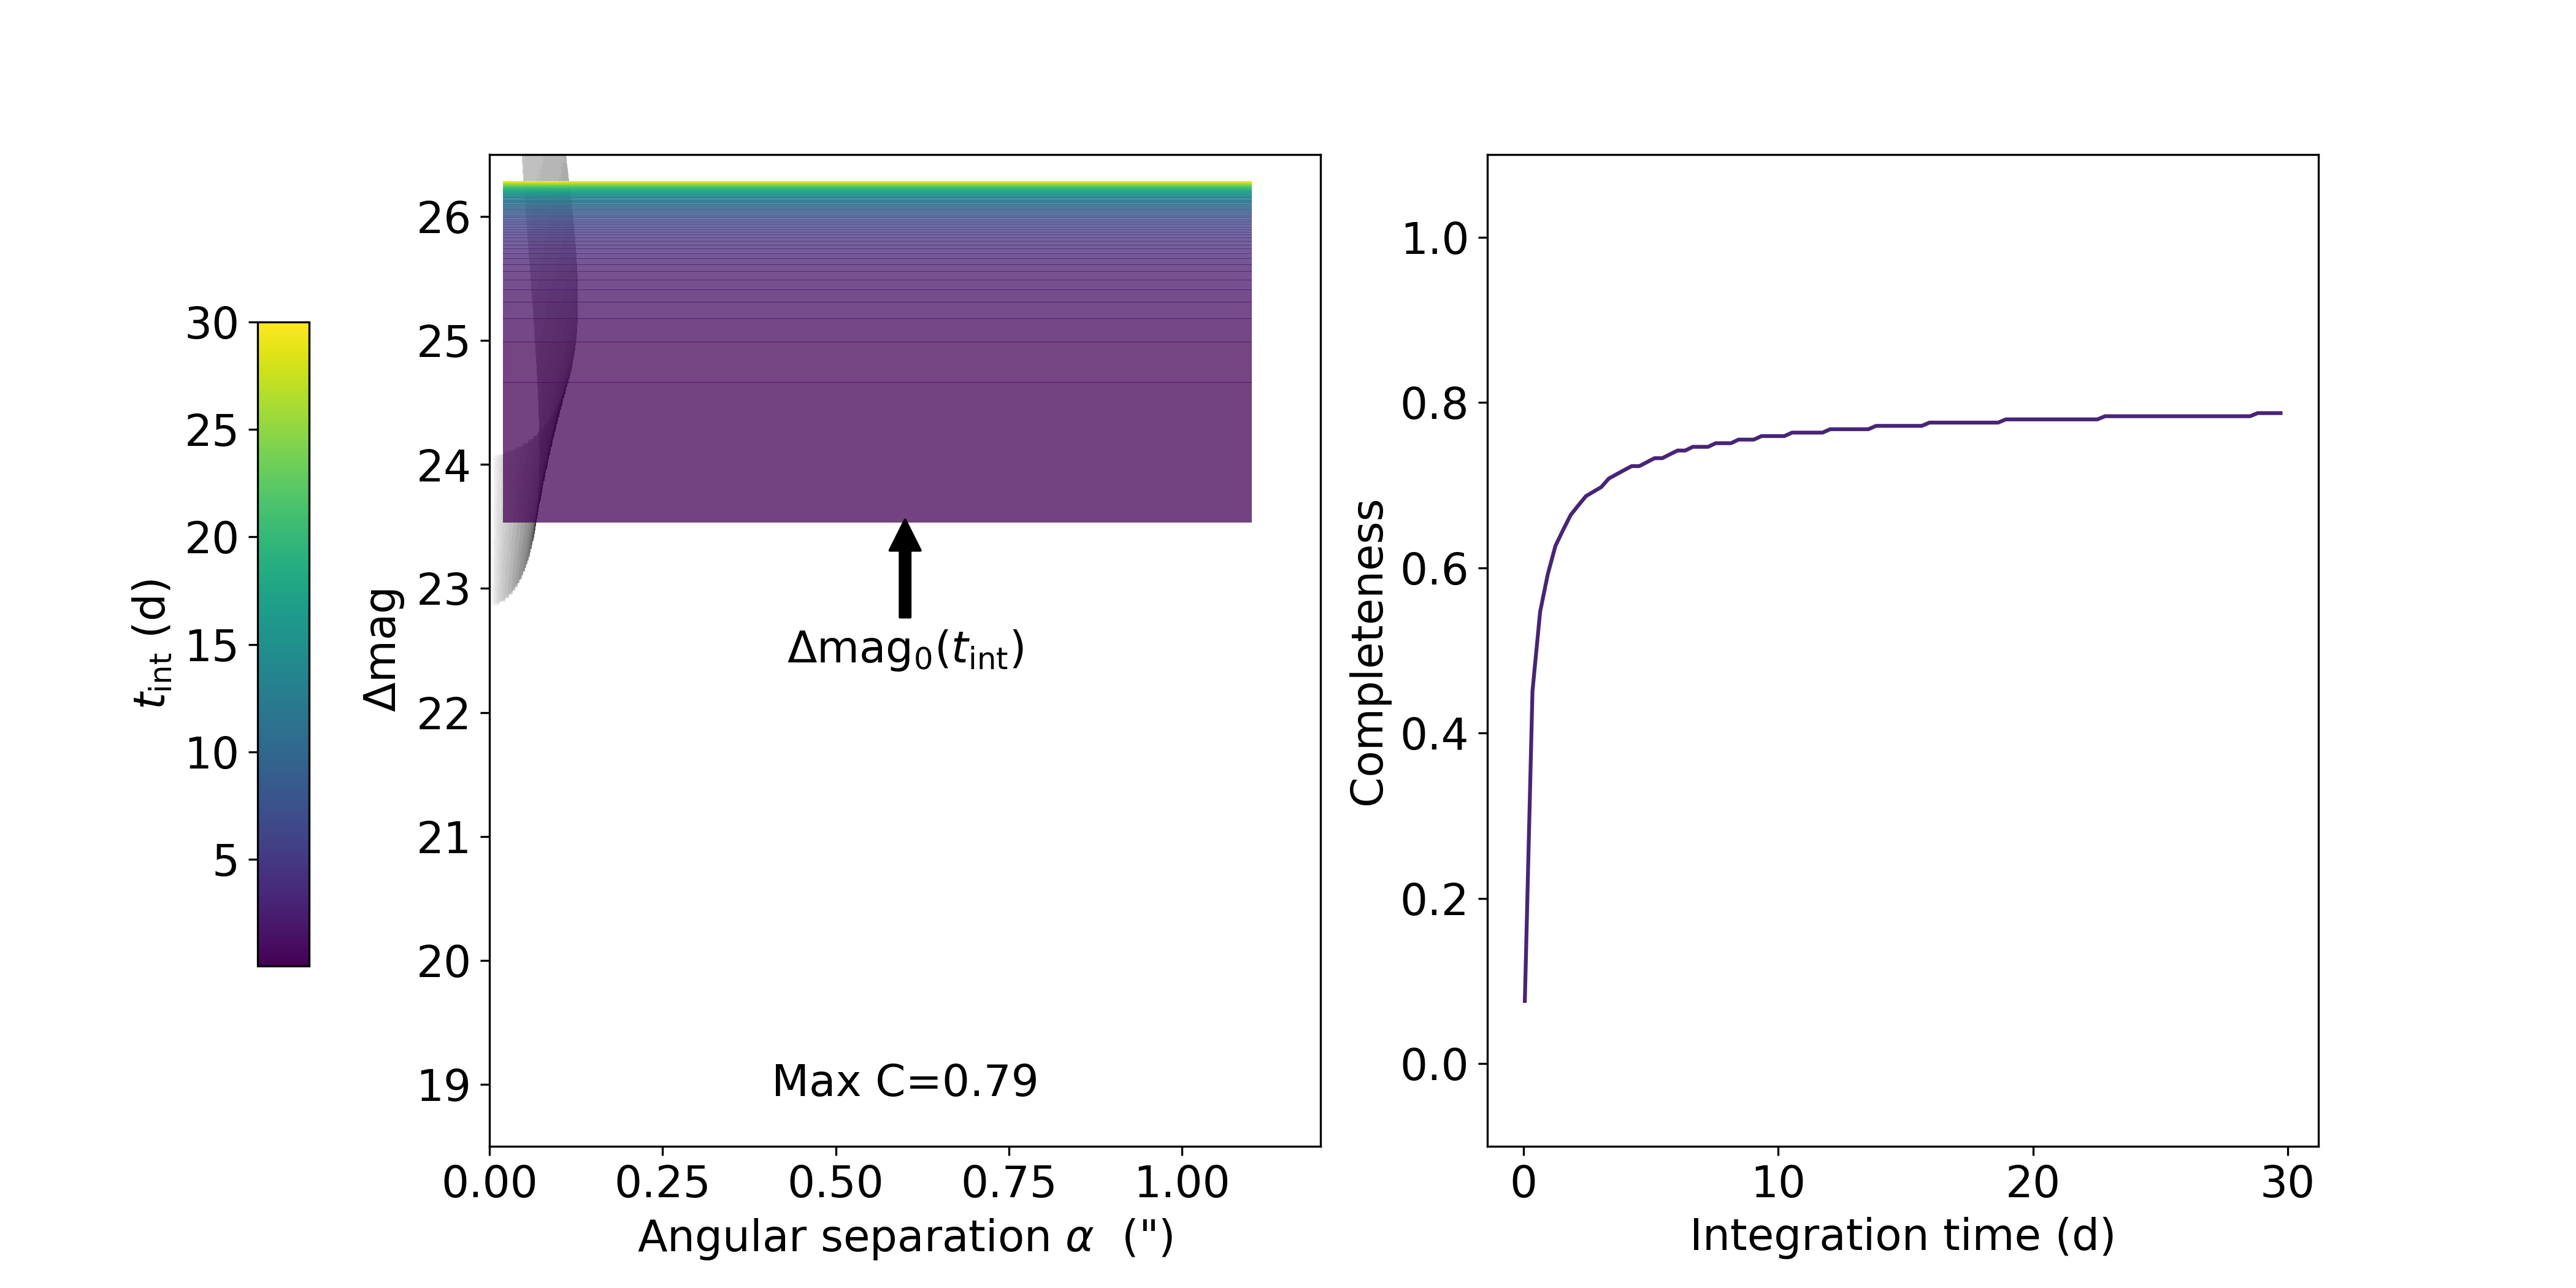
\includegraphics[width=0.95\textwidth]{ch3/figures/default_dmag_curve.png}
  \end{center}
  \caption{Plot of $\Delta\textrm{mag}_0(t_\textrm{int})$ values without separation dependence
  overlaid on the PDF of an Earth-like planet HIP 91438 ($\approx$13 parsecs from Earth)
  if observed with a prospective design of the Habitable Worlds Observatory.
  Completeness for 30 days of integration time is 0.8.}
  \label{fig:default_dmag_curve}
\end{figure}

A good place to start is calculating completeness
as a function of integration time $t_\textrm{int}$. An example
is shown in \Cref{fig:default_dmag_curve}, where the colored rectangle
represents the calculated $\Delta\textrm{mag}_0$ values for a range of
$t_\textrm{int}$ values with $\alpha$ held constant to the midpoint between
the IWA and OWA, $n_\textrm{EZ}=22 \frac{\textrm{mag}}{\textrm{arcsec}^2}$, and
$n_\textrm{Z}=23 \frac{\textrm{mag}}{\textrm{arcsec}^2}$. Because we have a
flat $\Delta\textrm{mag}_0$ the completeness can be calculated as
\begin{equation}
  c(t_\textrm{int}) = \int_{0}^{\Delta\textrm{mag}_0(t_\textrm{int})} 
  \int_{\alpha_\textrm{min}}^{\alpha_\textrm{max}} 
  f(\alpha, \Delta\textrm{mag})\textrm{d}\alpha \textrm{d}\Delta\textrm{mag}
  \label{eq:flat_comp_integral}
\end{equation}
where $f(\alpha, \Delta\textrm{mag})$ is the joint probability density function 
of an Earth-like planet population. In this scenario we see a very steep slope
initially and then little benefit after a few days of integration time.

% To reduce computation time
% $\Delta\textrm{mag}$ for a set of logarithmically spaced integration times we
% can interpolate smoothly and get the dimmest detectable $\Delta\textrm{mag}$
% for the star at an required integration time.



\subsection{Zodiacal light calculations}
\label{sub:zodi}

Local and exozodiacal light are calculated in the same manner as is used by
\code{EXOSIMS}, which is based on the work in \citet{leinert1997Reference1998,
starkMaximizingExoEarthCandidate2014,starkLowerLimitsAperture2015,
keithlyOptimalScheduling2020}. The specific intensity of local zodiacal
light is calculated as
\begin{equation}
  I_\textrm{zodi}(\Delta \lambda_\odot, \beta_\odot, \lambda_0) = 
  I_{\textrm{zodi}, \textbf{r}}^V(\Delta \lambda_\odot, \beta_\odot) 
\frac{I_{\textrm{zodi}, \lambda} (\lambda_0)}{I_{\textrm{zodi}, \lambda}(\textrm{500 nm})}
  \label{eq:local_zodi}
\end{equation}
where $I_{\textrm{zodi}, \lambda}$ is an interpolant over
\citet{leinert1997Reference1998} Table 19 for the specific intensity of
zodiacal light as a function of wavelength, $I_{\textrm{zodi},
\textbf{r}}^V(\Delta \lambda_\odot, \beta_\odot)$ is an interpolant over Table 17 of the same
paper and represents the specific intensity of zodiacal light as a function of
the telescope's look vector, $\Delta \lambda_\odot$ is the ecliptic
longitude of the target with respect to the current longitude of the sun,
$\beta_\odot$ is the ecliptic latitude, and $\lambda_0$ is the observing
wavelength. The units for \Cref{eq:local_zodi} are photons/s/m$^2$/as$^2$/nm.
For clarity, we will describe the zodiacal light in magnitude units by
converting the specific intensity into mag/as$^2$ units
\begin{equation}
  Z = -2.5 \log_{10}(I_\textrm{zodi}) \,.
  \label{eq:zodi_mag}
\end{equation}

The values of exozodiacal light are calculated in a
similar fashion but with a multiplication factor $n_{EZ}$ to allow for
planetary systems with more or less dust than the solar system. The calculation
for the specific intensity of exozodiacal light in V band is
\begin{equation}
  I_\textrm{exozodi}^V = n_{EZ} \mathcal{F}_{0,V}10^{-0.4(M_V-M_{V,\odot}+x)}\left( \frac{1 \textrm{AU}}{r}\right)^2
  \label{eq:exozodi}
\end{equation}
where $n_{EZ}$ is the number of zodi in the planetary system (where 1 ``zodi'' is
equivalent to the exact distribution of dust in the solar system), $M_V$ is the
absolute magnitude of the target star, $M_{V,\odot}$ is the absolute magnitude
of the sun, $x$ is the nominal specific brightness of the planetary system's
disk at 1 AU ($22\textrm{ mag }\textrm{as}^{-2}$), and $r$ is the planet's orbital radius at the time of
observation. To get the specific intensity at an arbitrary wavelength we can
then use $I_\textrm{exozodi}^V$ instead of $I_{\textrm{zodi}, \textbf{r}}^V$ in
\Cref{eq:local_zodi}. To calculate the specific intensity of the planet at a
given time we calculate its $r$ value and the corresponding specific intensity.
In this chapter, we parameterize the exozodi values with the $n_{EZ}$ value. To
sample $n_{EZ}$ we use the distribution of exozodi from
\citet{ertelHOSTSSurvey2020} which extrapolates the results of the Large
Binocular Telescope Interferometer's (LBTI) ``Hunt for Observable Signatures of
Terrestrial planetary Systems'' (HOSTS) survey to get a distribution of
exozodiacal dust.


% Extra zodiacal light is unlikely to be known before a mission, but
% is worth keeping as an input so that different scenarios can be tested quickly.
% The zodiacal light can be estimated as a function of time if a telescope's
% orbit is known. However, in summed completeness simulations the time of
% observation is generally not considered so it would be of little use. 

\subsection{Full Photometric Constraint}
\label{sub:full_comp}
\begin{figure}
  \begin{center}
    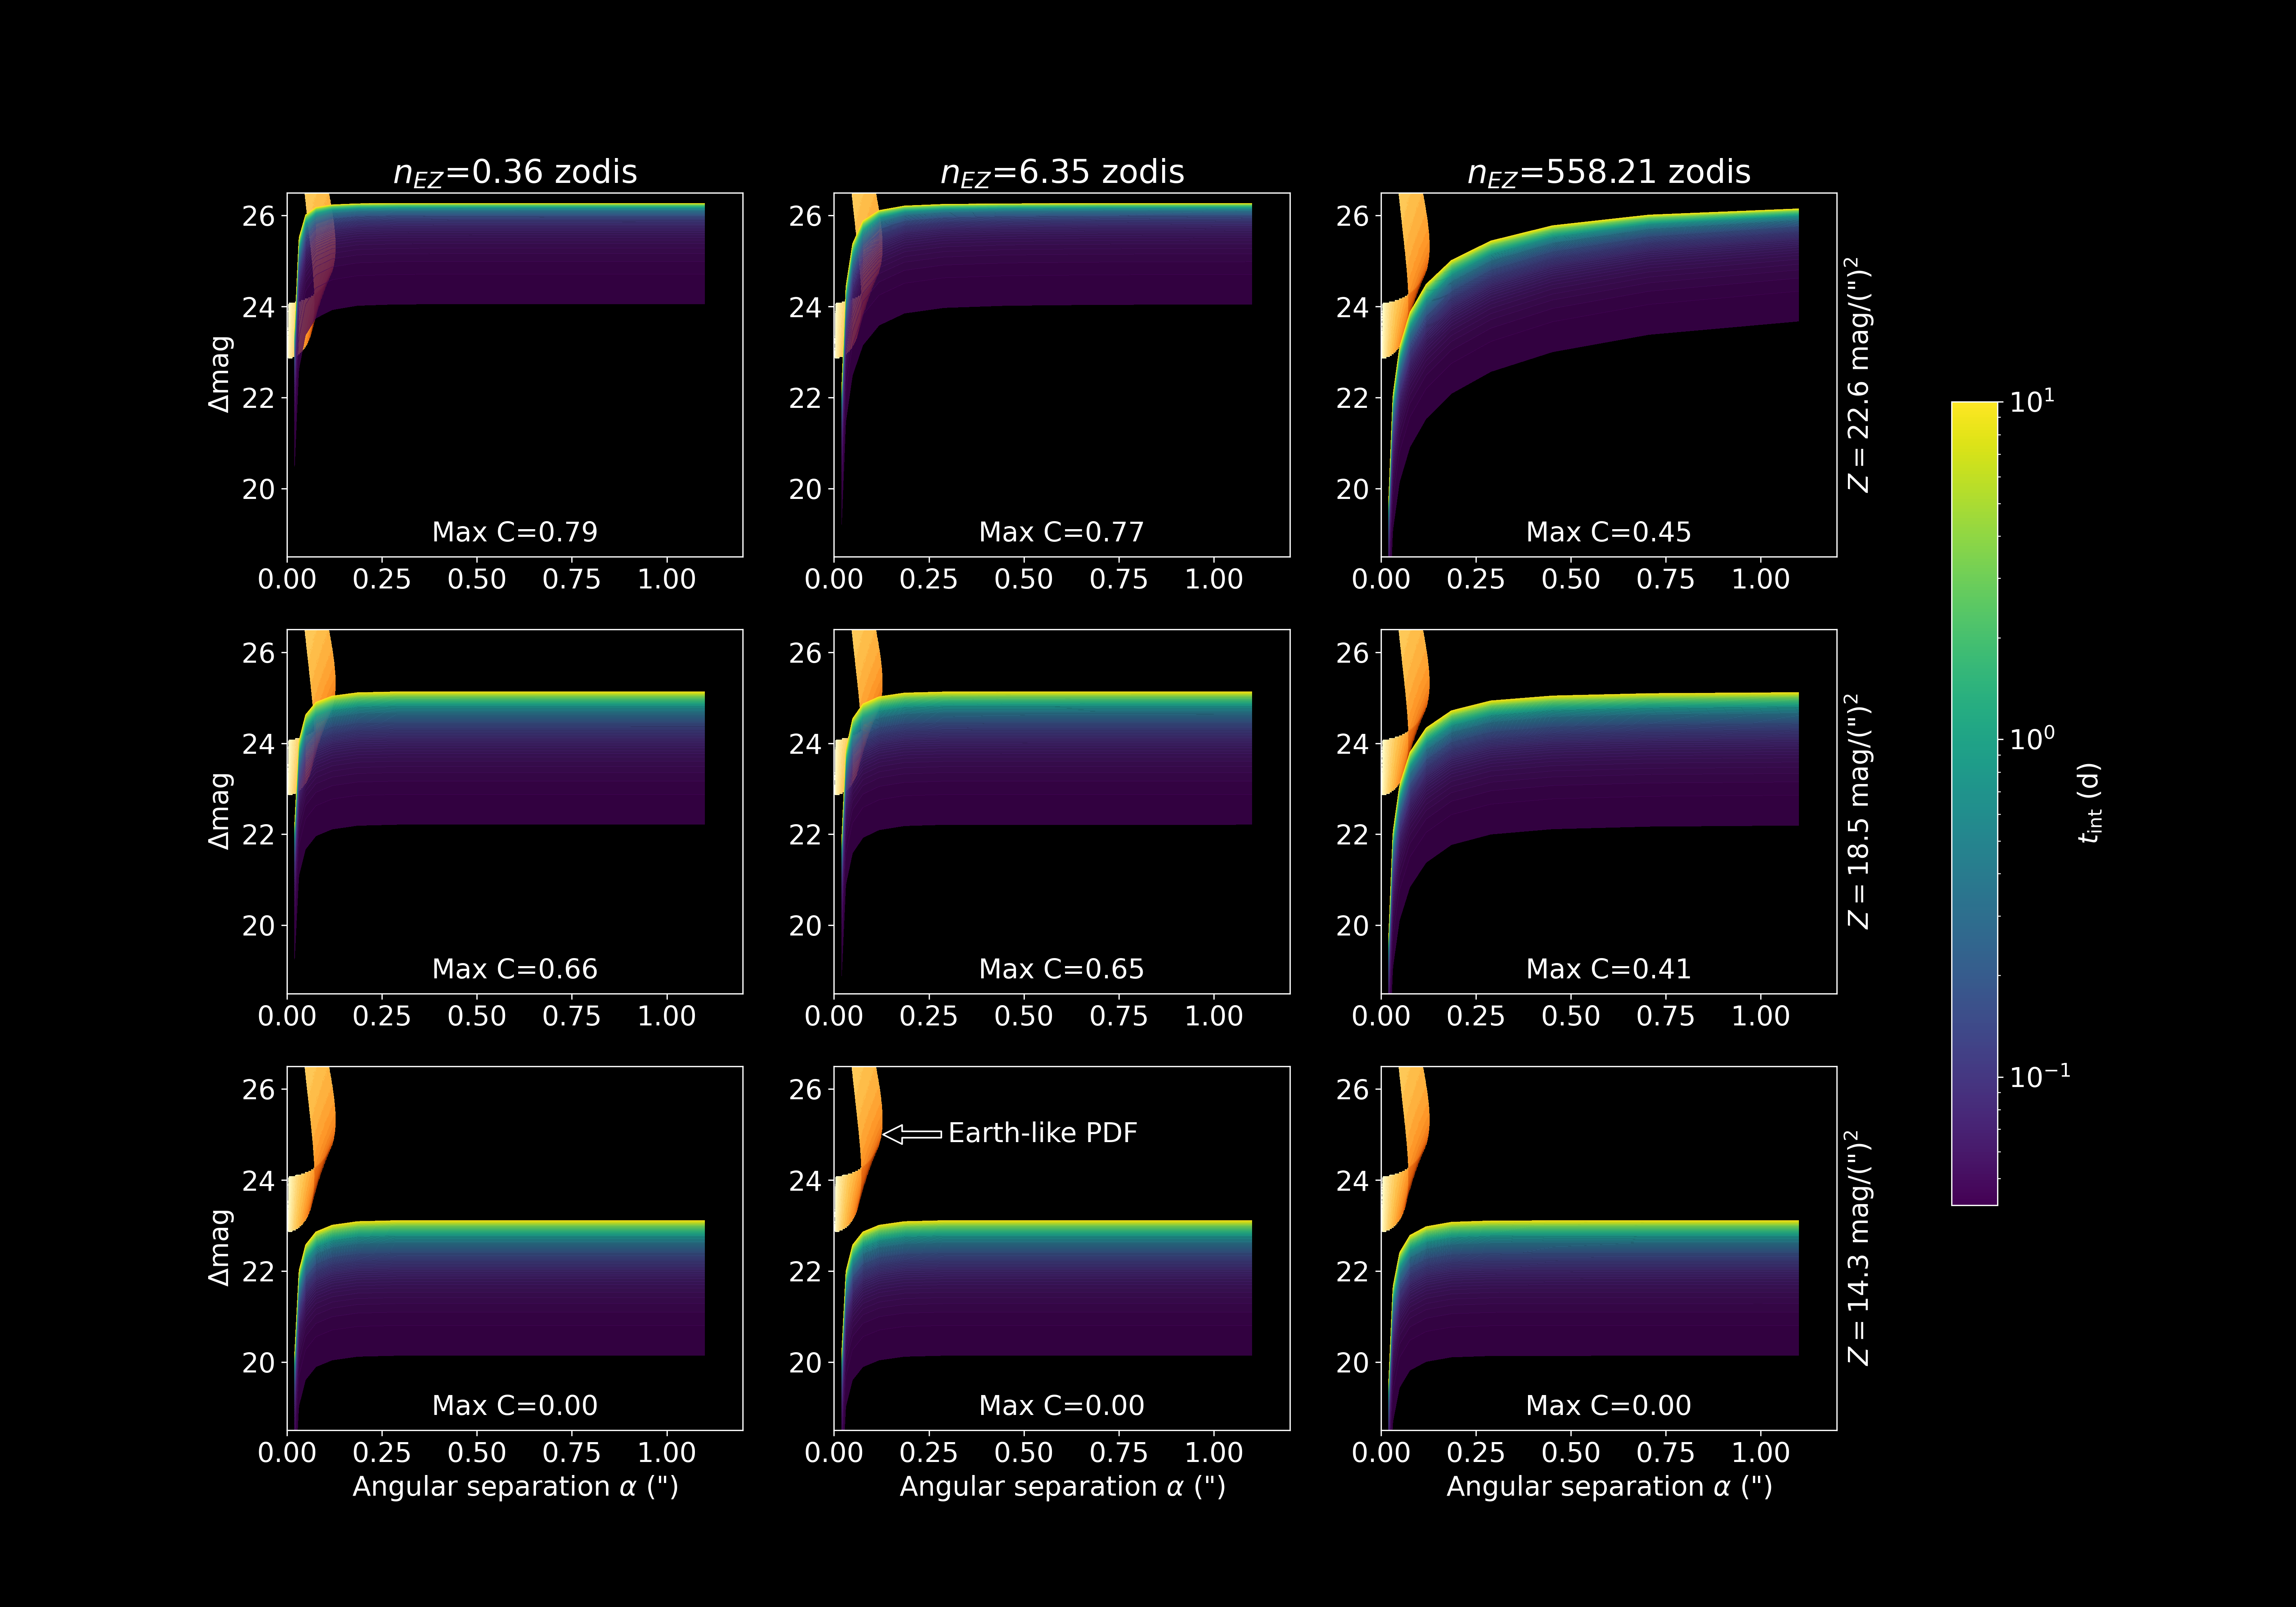
\includegraphics[width=0.95\textwidth]{ch3/figures/fZ_fEZ_curves.pdf}
  \end{center}
  \caption{$\Delta\textrm{mag}_0(t_\textrm{int}, \alpha, Z, n_\textrm{EZ})$ for HIP 91438.
    Each column has a constant value of $n_\textrm{EZ}$ and each row has a
    constant value of $Z$. The zodiacal light values were generated
    using EXOSIMS to simulate the range of zodiacal light values of observing
  the star for a telescope at L2.}
  \label{fig:fZ_fEZ_curves}
\end{figure}

By accounting for integration time, separation, local zodiacal light, and 
exozodiacal light we end up with a four dimensional photometric constraint for
each star, $\Delta\textrm{mag}_0(t_\textrm{int}, \alpha, Z,
n_\textrm{EZ})$. These four dimensions are the range of input values necessary
to invert the exposure time calculator described by \citet{Nemati2014} for a
specific mission design. An example of the $\Delta\textrm{mag}_0$ curves for
various zodiacal light assumptions is shown in \Cref{fig:fZ_fEZ_curves}. 
To visualize the impact of separation and zodiacal light on completeness
we can formulate our limiting $\Delta\textrm{mag}$ as 
$\Delta\textrm{mag}_0(t_\textrm{int}, \alpha, Z, n_\textrm{EZ})$.
Then our equation for completeness becomes
\begin{equation}
  c(t_\textrm{int}, Z, n_\textrm{EZ}) = 
  \int_{\alpha_\textrm{min}}^{\alpha_\textrm{max}} 
  \int_{0}^{\Delta\textrm{mag}_0(t_\textrm{int}, \alpha, Z, n_\textrm{EZ})}
  f(\alpha, \Delta\textrm{mag})\textrm{d}\alpha \textrm{d}\Delta\textrm{mag}
  \label{eq:comp_integral}
\end{equation}
where we leave our zodiacal light values as inputs. In the best case scenario,
the completeness is within 0.01 of the flat curve shown in
\Cref{fig:default_dmag_curve}, but drops considerably for high exozodiacal
light values.

\begin{figure}
  \begin{center}
    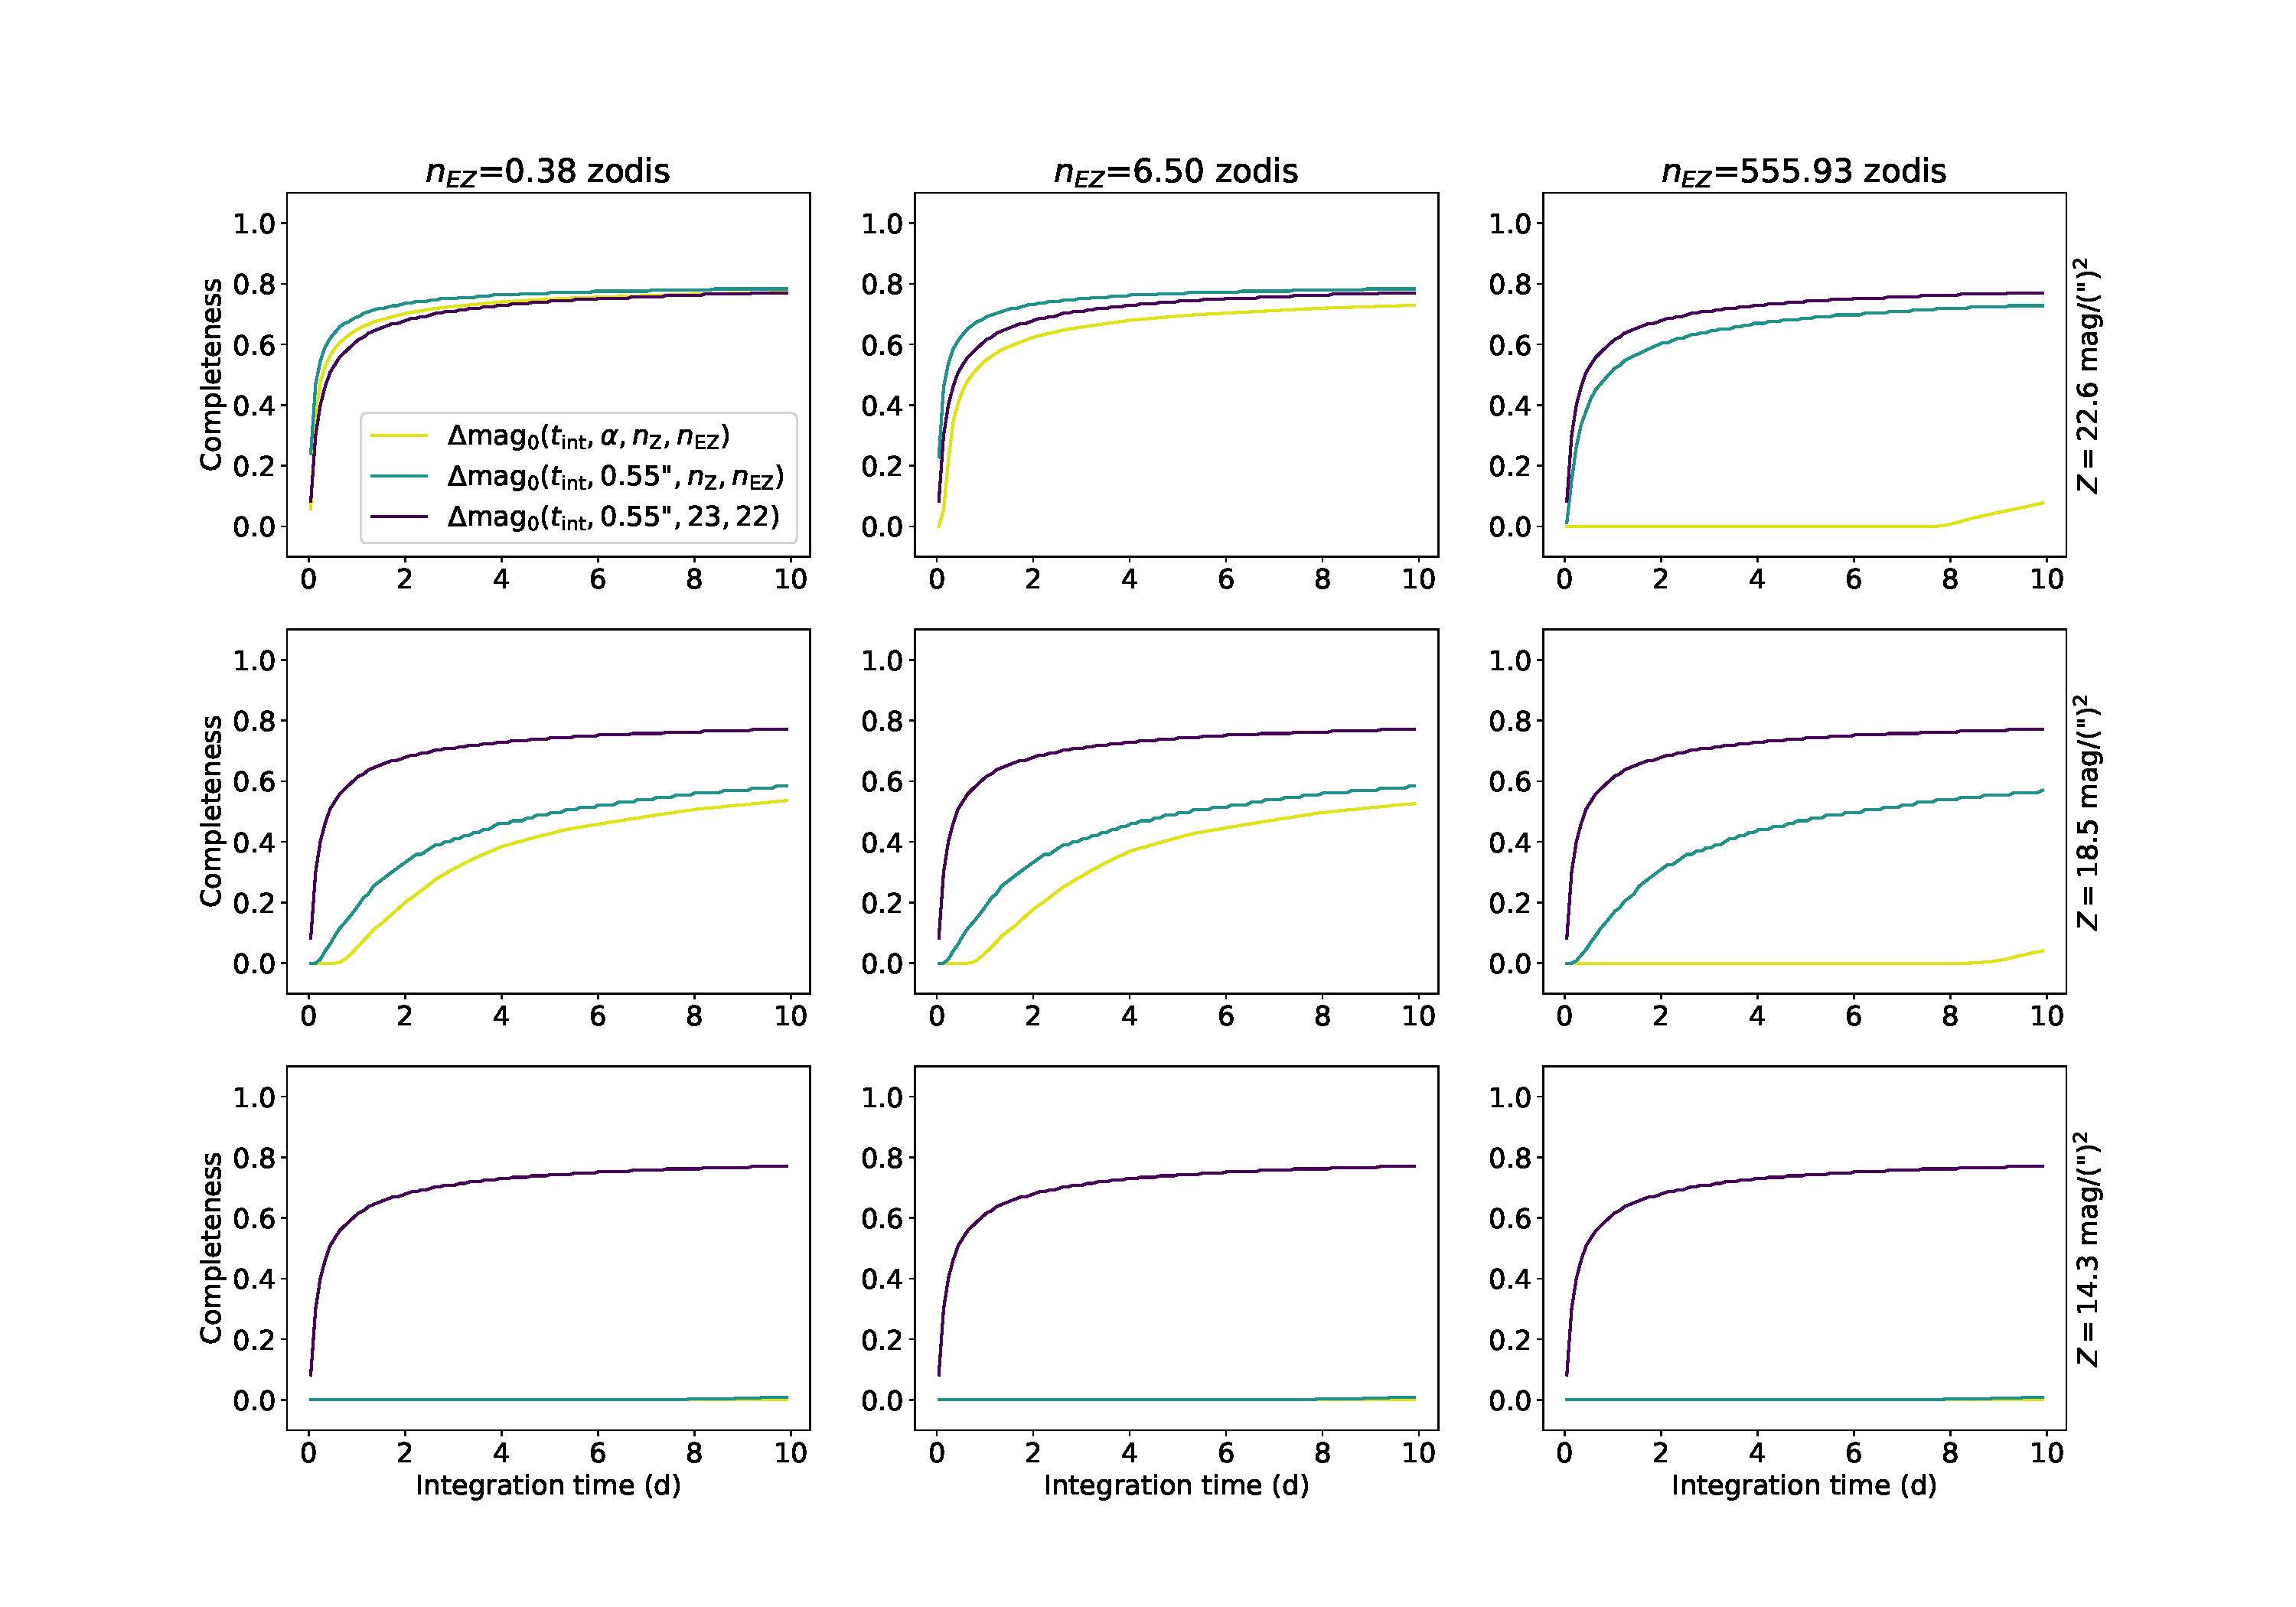
\includegraphics[width=\textwidth]{ch3/figures/Z_EZ_comps_flat.pdf}
  \end{center}
  \caption{Completeness as a function of integration time for the same astrophysical
  scenarios as in \Cref{fig:fZ_fEZ_curves}. The three lines represent different levels
  of accounting for separation and zodiacal light. The line for
  $\Delta\textrm{mag}_0(t_\textrm{int}, \alpha, Z, n_\textrm{EZ})$
  is the most accurate as it accounts for the most variables and is 
  found by applying \Cref{eq:comp_integral} to the curve in \Cref{fig:fZ_fEZ_curves}.
  The 
  $\Delta\textrm{mag}_0(t_\textrm{int}, 0.55\textrm{as}, Z, n_\textrm{EZ})$
  line shows the effect of calculating the completeness without accounting for
  the drop in $\Delta\textrm{mag}_0$ at small separations. And the
  $\Delta\mathrm{mag}_0(t_\mathrm{int}, 0.55$\textrm{as}$, 23 (\textrm{mag}/\textrm{as})^2, 22(\textrm{mag}/\textrm{as})^2)$
  line is an overlay of the curve generated in \Cref{fig:default_dmag_curve}.
  }
  \label{fig:fZ_fEZ_comps}
\end{figure}

\begin{figure}
  \begin{center}
    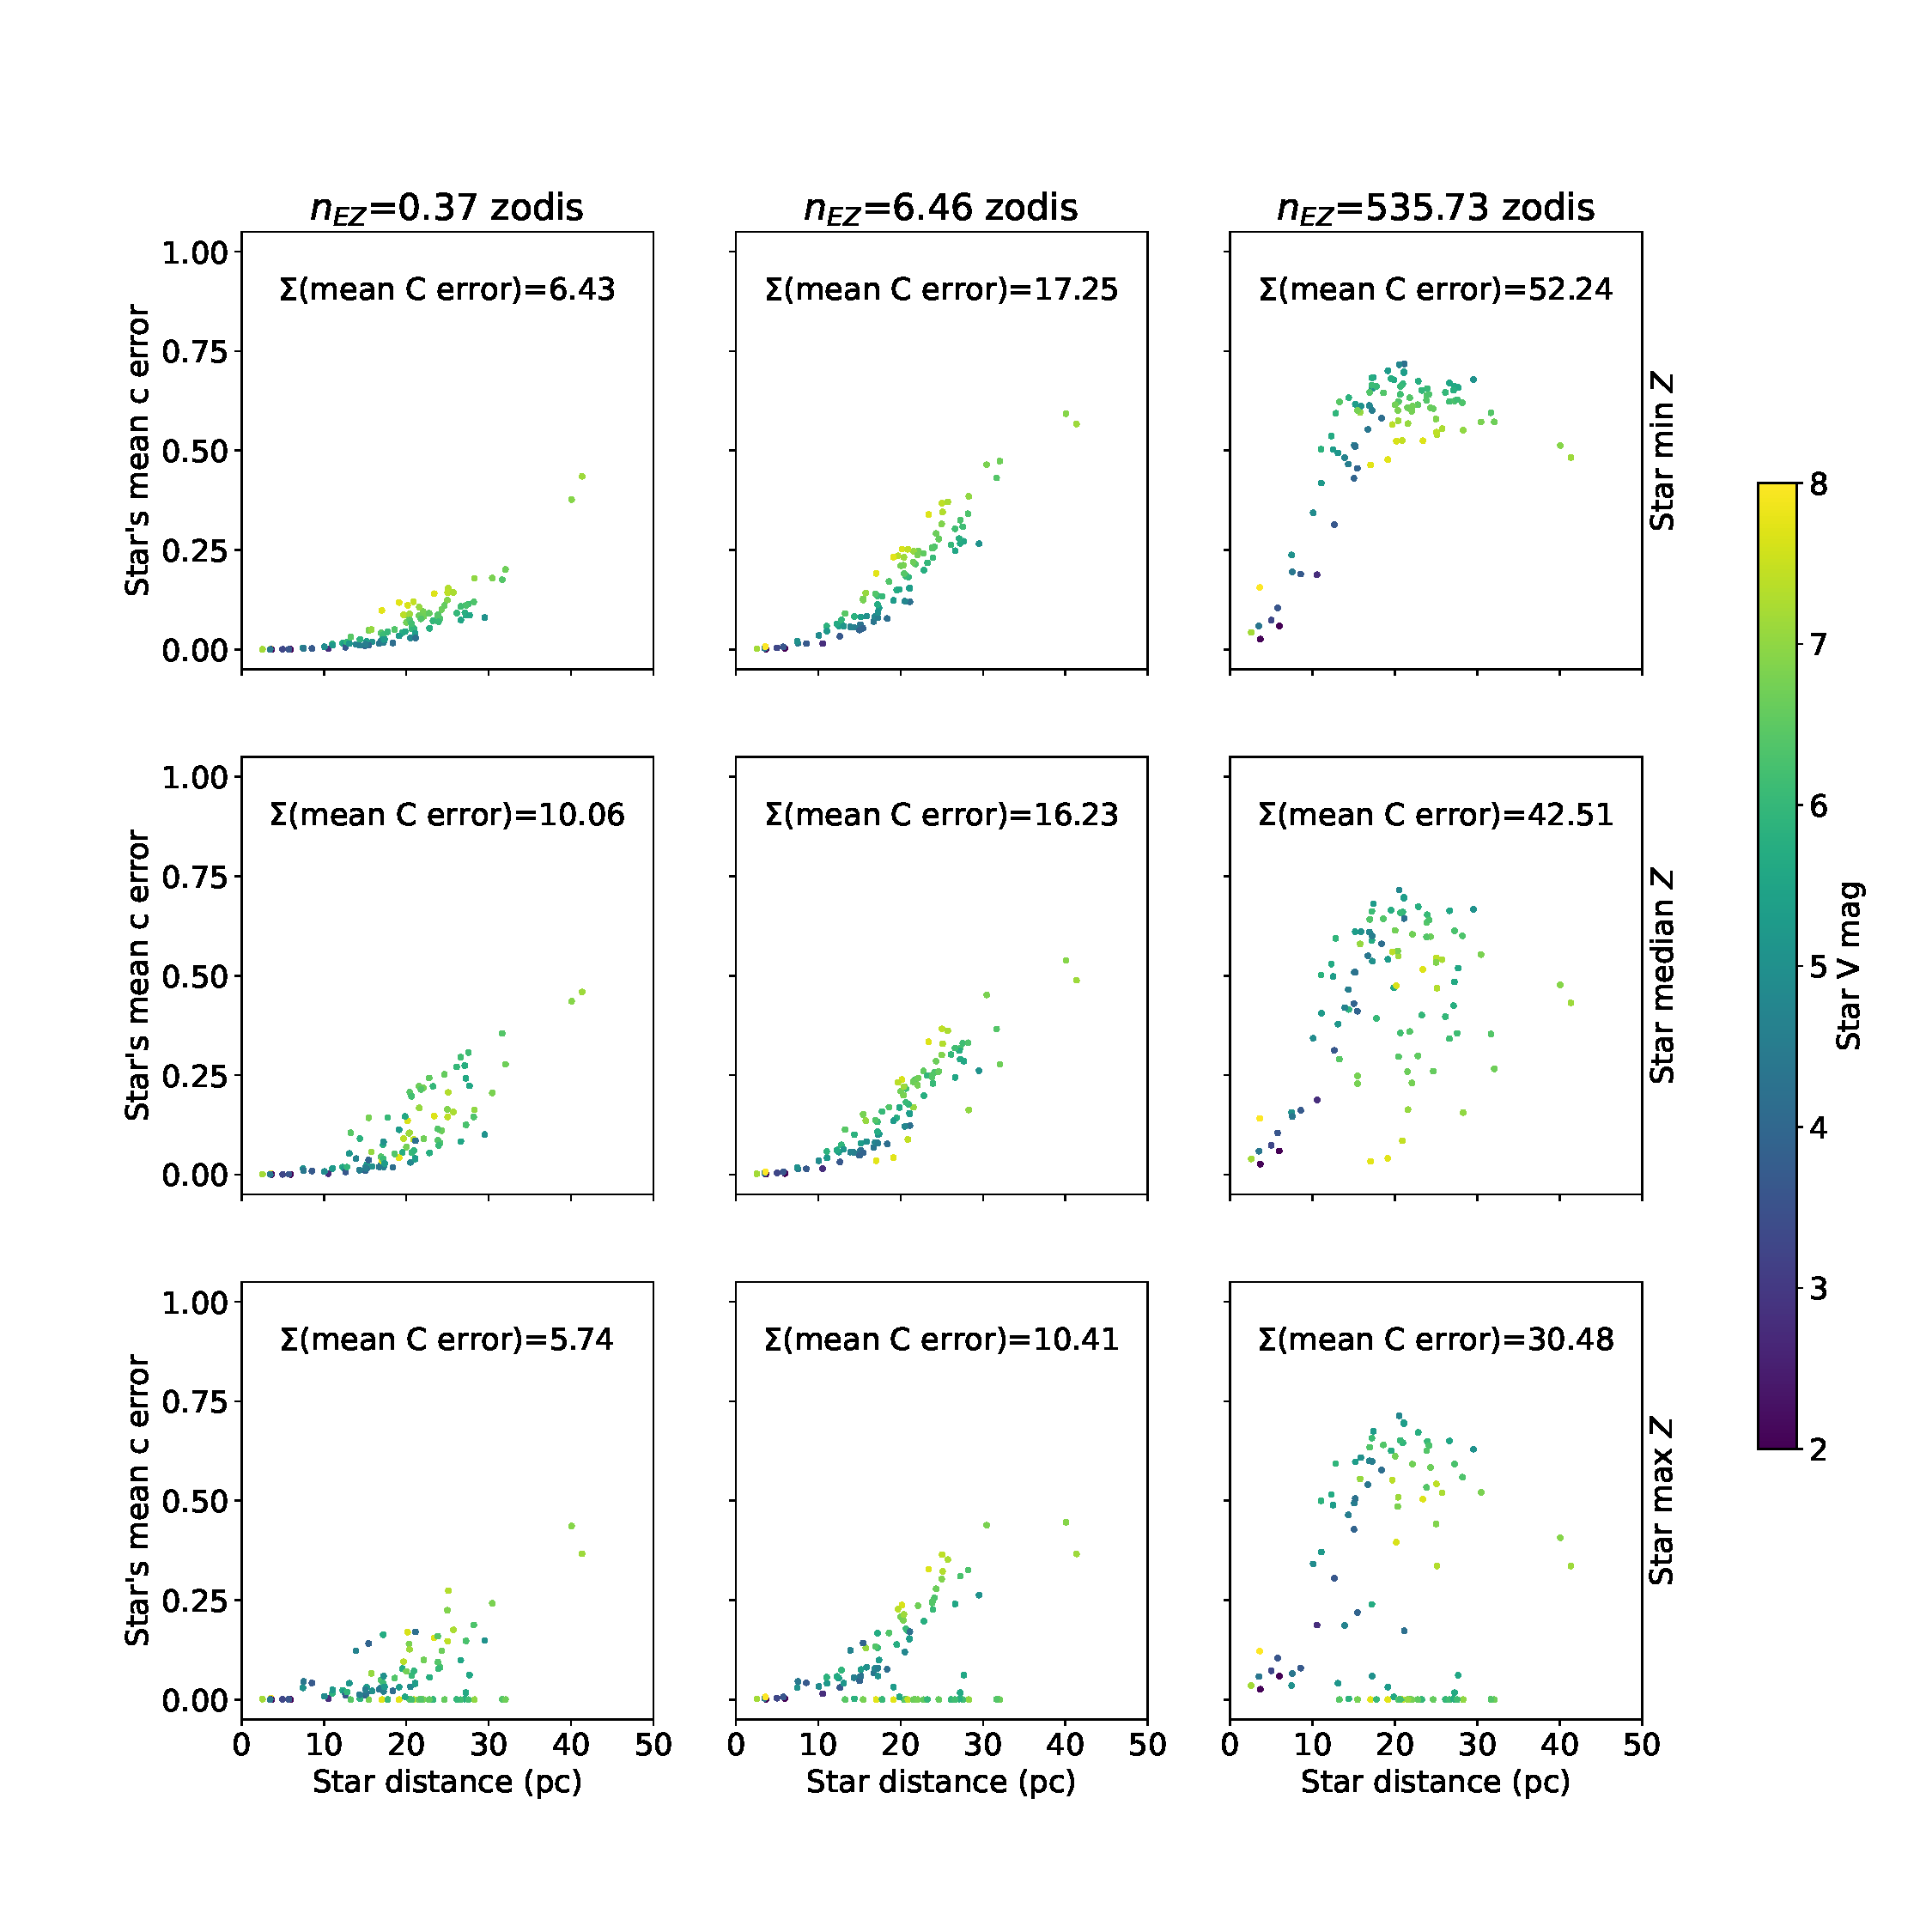
\includegraphics[width=0.95\textwidth]{ch3/figures/mean_comp_errors.pdf}
  \end{center}
  \caption{Mean completeness error for different stars calculated as the mean difference between
  the default curve and the scenario curve in \Cref{fig:fZ_fEZ_comps} for each star. The columns represent
  different amounts of exozodiacal dust and the rows show the star's minimum, median, and maximum zodiacal
  light surface brightness for a telescope on an L2 orbit. The increase in 
  mean completeness error as star distance increases shows that not accounting for the effects of
  $\alpha$ on $\Delta\textrm{mag}_0$ leads to a systematic overestimation of completeness. 
  The effect becomes more pronounced for greater amounts of exozodiacal dust 
  assumed.}
  \label{fig:mean_comp_errors}
\end{figure}

To see the effect on completeness more clearly \Cref{fig:fZ_fEZ_comps} shows
completeness as a function of integration time for the various scenarios in
\Cref{fig:fZ_fEZ_curves} and compares them to the completeness curves generated
with less complete information. All of the values shown in
\Cref{fig:default_dmag_curve,fig:fZ_fEZ_curves,fig:fZ_fEZ_comps} are for a
single star and demonstrate the large trade space inherent to making
assumptions on the zodiacal light when maximizing completeness. Without
ensuring that observations are made near the minimum local zodiacal light value
a high completeness observation can drop to zero completeness. Values of
exozodiacal light are unlikely to be known before an initial observation is
made so it cannot be accounted for other than choosing an assumed $n_\textrm{EZ}$
value.

\Cref{fig:mean_comp_errors} summarizes the effect of using the optimistic
``default'' scenario of a flat limiting $\Delta\textrm{mag}$ per integration
time. The targets shown are the 97 stars from the NEID Earth Twin Survey with
full stellar information in the Simbad database
\citep{guptaTargetPrioritization2021}. For each star the
$\Delta\textrm{mag}_0$ values are generated. Then the completeness per
integration time function is generated for both the case when
$\Delta\textrm{mag}_0$ is assumed to be flat and the case that takes separation
into account, similar to \Cref{fig:fZ_fEZ_comps}. We average the distance
between the two completeness per integration time functions and plot them as a
single point in \Cref{fig:mean_comp_errors}. It's clear that the change in
limiting $\Delta\textrm{mag}$ near the IWA becomes a problem past 10 parsecs.
For extreme exozodiacal light values the effect becomes much more pronounced.

For yield modeling based on Monte Carlo mission simulations, such as EXOSIMS
\citep{savranskyWFIRSTAFTACoronagraphScience2015, delacroixScienceYield2016,
savranskyEXOSIMSExoplanetOpenSource2017}, the $\Delta\textrm{mag}_0$ values for
a star can be reused across mission simulations with the same telescope orbit
and optical system. Calculating the 2000 $\Delta\textrm{mag}_0$ values to
account for all combinations of 10 $\alpha$ values, 20 $t_\textrm{int}$ values,
and 10 $Z$ values takes 20-30 seconds to run on a Ryzen 5800x 8 core processor
in parallel. An application of this could be to schedule observations when
accounting for the zodiacal light without requiring observations be made at the
zodiacal light minimum, as was done in \citet{keithlyOptimalScheduling2020}. In
that scheduler observations are all made at the minimum zodiacal light for the
target star. By allowing for observations at times near the minimum, the
scheduler can likely make worthwhile trades between targets.

% \subsection{TODO:Exozodi calculations}
% Given a distribution of zodi values for a planetary system we could marginalize
% over it to calculate the completeness with respect to the possible zodi values
% of an unknown planetary system.
% \begin{equation}
%   c(t_\textrm{int}, n_\textrm{Z}) = 
%   \int_{n_\textrm{EZ,min}}^{n\textrm{EZ,max}} 
%   \int_{\alpha_\textrm{min}}^{\alpha_\textrm{max}} 
%   \int_{0}^{\Delta\textrm{mag}_0(t_\textrm{int}, \alpha, n_\textrm{Z}, n_\textrm{EZ})}
%   f(\alpha, \Delta\textrm{mag}) g(n_\textrm{EZ})
%   \textrm{d}\alpha \textrm{d}\Delta\textrm{mag} \textrm{d}n_\textrm{EZ}
%   \label{eq:comp_integral_nEZ}
% \end{equation}
% where $g(n_\textrm{EZ})$ is the density function of $n_\textrm{EZ}$.

% The reason to include separation in the formulation of the photometric
% constraint is shown in The traditional set of dimmest detectable
% $\Delta\textrm{mag}$ values is shown in 

\section{Probability of Detection} % (fold)
\label{section:impact_on_pdet}

An interesting challenge for direct imaging is using the orbit fits from
indirect exoplanet detection techniques to estimate the best times to make
direct observations. Indirect detection via the radial velocity method cannot
separate the mass and inclination of a planet's orbit, which complicates direct
imaging scheduling because the inclination is important for the planet-star
separation and the mass is used to estimate radius which impacts the brightness
of the planet. Chapter 2 showed how to take a radial velocity fit and generate
the most likely times the planet will be detectable for a given instrument.
Notably missing from that work was considerations of integration time and
zodiacal light conditions.

For a star with a planet fitted via the radial velocity method we can calculate
the dimmest detectable $\Delta\textrm{mag}$ curves, the $\Delta\textrm{mag}_0$
values, for a telescope's orbit and optical system by looping over the zodiacal
light values for the star during the mission, the separations between the
instrument's IWA and OWA, and integration times spaced logarithmically between
the minimum and maximum allowed integration times. Logarithmic spacing is
useful as the largest changes in $\Delta\textrm{mag}_0$ occur at small
integration times and because $\Delta\textrm{mag}$ is a logarithmic quantity
while time is linear. In testing, we found that the most useful process was
calculating 2d interpolants that return the dimmest detectable
$\Delta\textrm{mag}$ given an integration time and separation. We generate a 2d
interpolant for a set of 10 zodiacal values between the star's minimum and
maximum zodiacal light surface brightness during the telescope's orbit. 

Exozodiacal light is treated similarly to the local zodiacal light in that it
is not included in the interpolants. Unlike the zodiacal light, we cannot come
up with the surface brightnesses directly, instead, we generate a range of
$n_\textrm{EZ}$ ``zodis'' as defined by
\citet{starkMaximizingExoEarthCandidate2014} and calculate the 2d interpolants
for a single value of $n_\textrm{EZ}$. For every $\alpha$ in the interpolant
the exozodiacal light surface brightness is calculated as if the planet is at
$\alpha$ value with an inclination of $135\degree$. Calculating it in this
fashion includes the fact that the exozodiacal light decreases for distant
orbits.

Using the dimmest detectable $\Delta\textrm{mag}$ curves to calculate
the probability of detection is useful because it means we do not need to calculate
the signal to noise ratio of every one of the orbit fits at every possible
observation time for all integration times. Instead, we propagate to time $t$ in
($\alpha$, $\Delta\textrm{mag}$) space with the method shown in
\Cref{cha:first_paper}, get the interpolant corresponding to the local zodiacal
light for the target star at $t$, and call that 2d interpolant with all the
$\alpha$ and integration times which returns the dimmest detectable
$\Delta\textrm{mag}$ values of interest. Then the probability of detection for
an integration time is a simple percentage of the number of
$\Delta\textrm{mag}$ values from propagation that are above their corresponding
$\Delta\textrm{mag}_0$ values, or
\begin{equation}
  P_\textrm{det}(t, t_\textrm{int}, Z, n_\textrm{EZ}) = 
  \int_{\alpha_\textrm{min}}^{\alpha_\textrm{max}} 
  \int_{0}^{\Delta\textrm{mag}_0(t_\textrm{int}, \alpha, Z, n_\textrm{EZ})}
  f(\alpha, \Delta\textrm{mag})\textrm{d}\alpha \textrm{d}\Delta\textrm{mag}
  \label{eq:comp_integral}
\end{equation}

\subsection{Validation}

\begin{figure}
  \begin{center}
    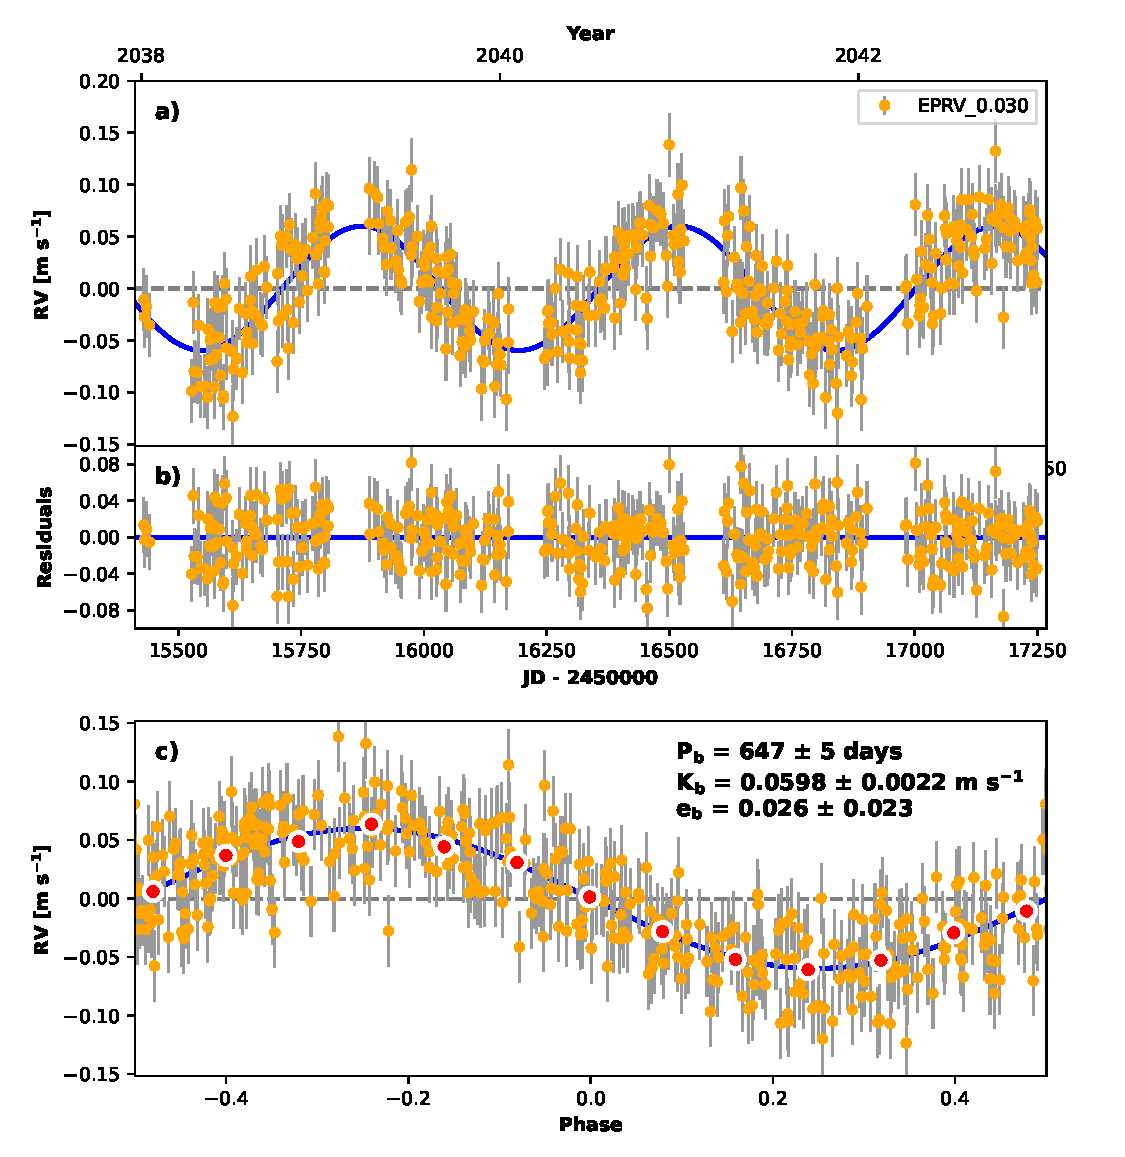
\includegraphics[width=0.95\textwidth]{ch3/figures/orbit_plot_mc_HIP_91438.pdf}
  \end{center}
  \caption{Radial velocity orbit fit of a habitable zone planet on a nearly edge on orbit from
  simulated extreme precision radial velocity data. Fit was done using
  \code{RVSearch}
  \citep{rosenthalCaliforniaLegacy2021}. Top row
  (a) overlays the observed RV data on the fitted planet's RV signal. Middle
  row (b) shows the residual RV signal when the fitted planet's RV signal is
  subtracted. The bottom row (c) shows the fitted planet's signal over a single
  period and the observed RV data phase folded into a single period. The bottom row
  additionally marks the planet's fitted period $P$, eccentricity $e$, and RV
  semi-amplitude $K$. The fit shows strong agreement with the underlying signal
  because the fitted orbital parameters are all within two standard deviations of the true
  planet orbital parameters.}
  \label{fig:rv_fit}
\end{figure}

\begin{figure}
  \begin{center}
    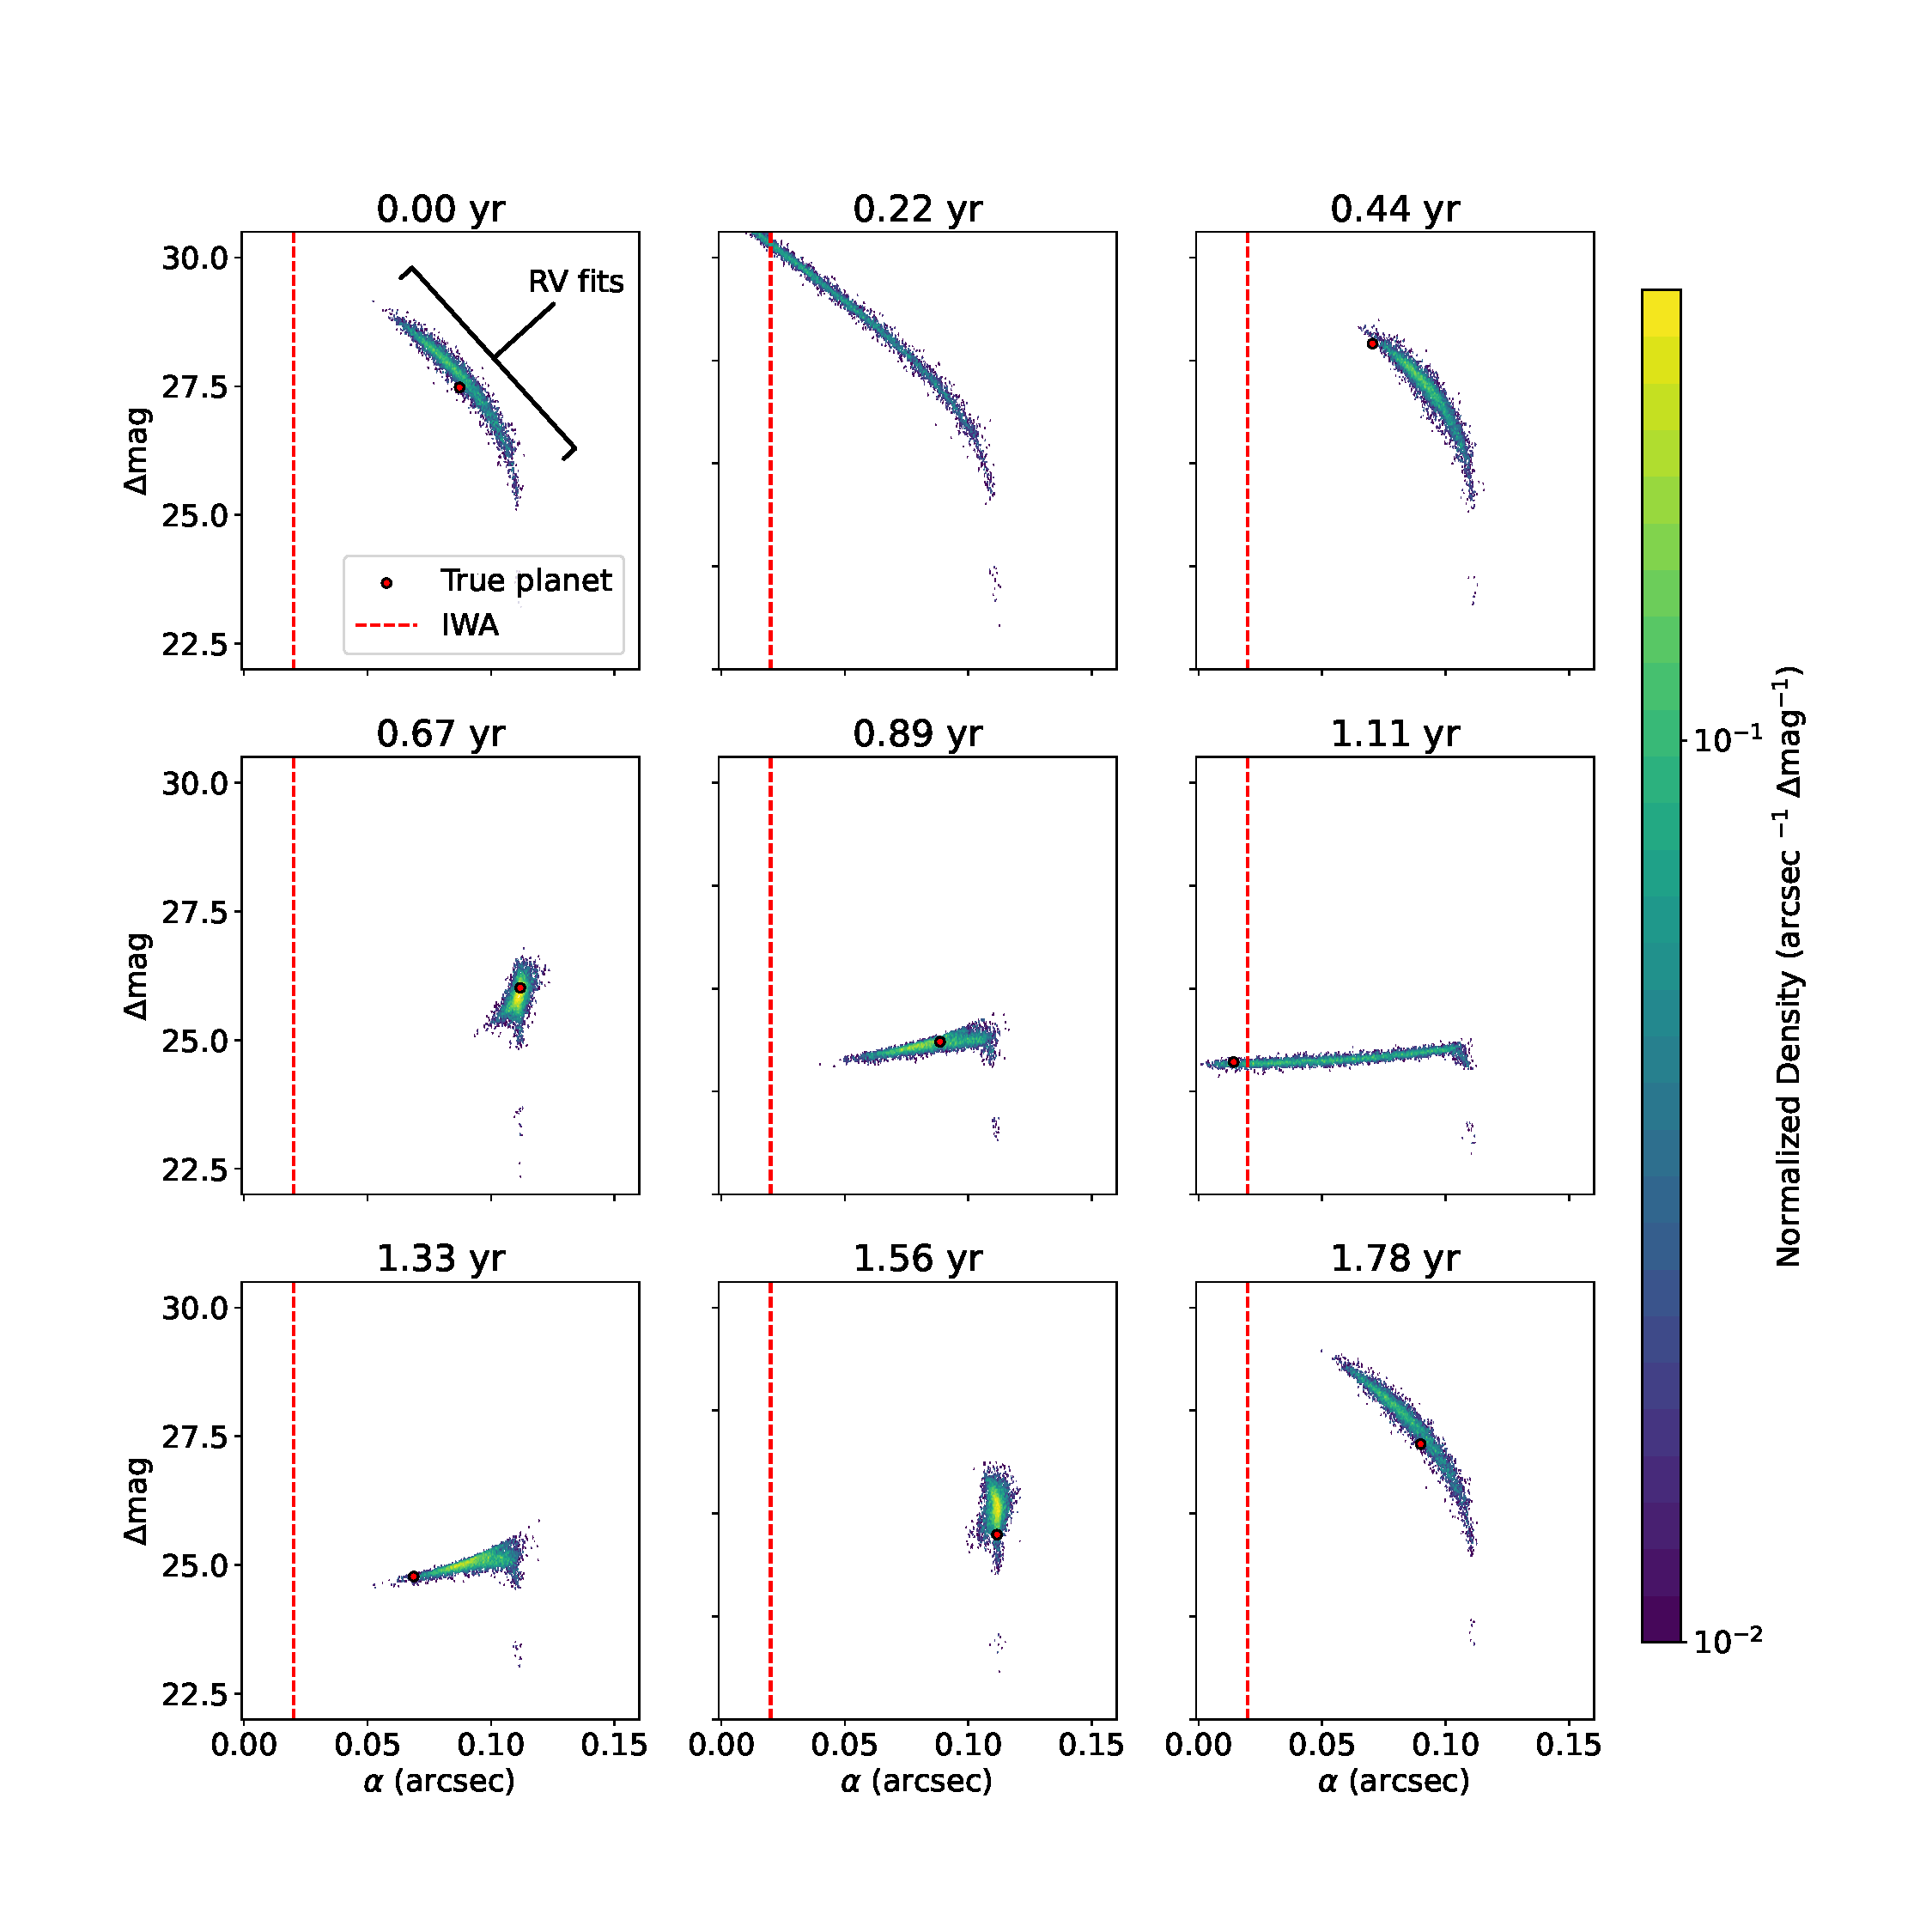
\includegraphics[width=0.95\textwidth]{ch3/figures/pop_propagation_in_time.pdf}
  \end{center}
  \caption{Propagation of the fitted orbits from \Cref{fig:rv_fit} compared to
    the propagation of the true planet. Each subplot is titled with the length
    of time passed since the final RV observation was made. The true planet remains
    within the set of fitted orbits which shows the fitted orbits are
  accurately describing the planet's $\alpha$ and $\Delta\textrm{mag}$ values. Because
  the fit had small errors on the orbital parameters there is very little dispersion
  among the fitted orbits.}
  \label{fig:pop_propagation_in_time}
\end{figure}

\begin{figure}
  \begin{center}
    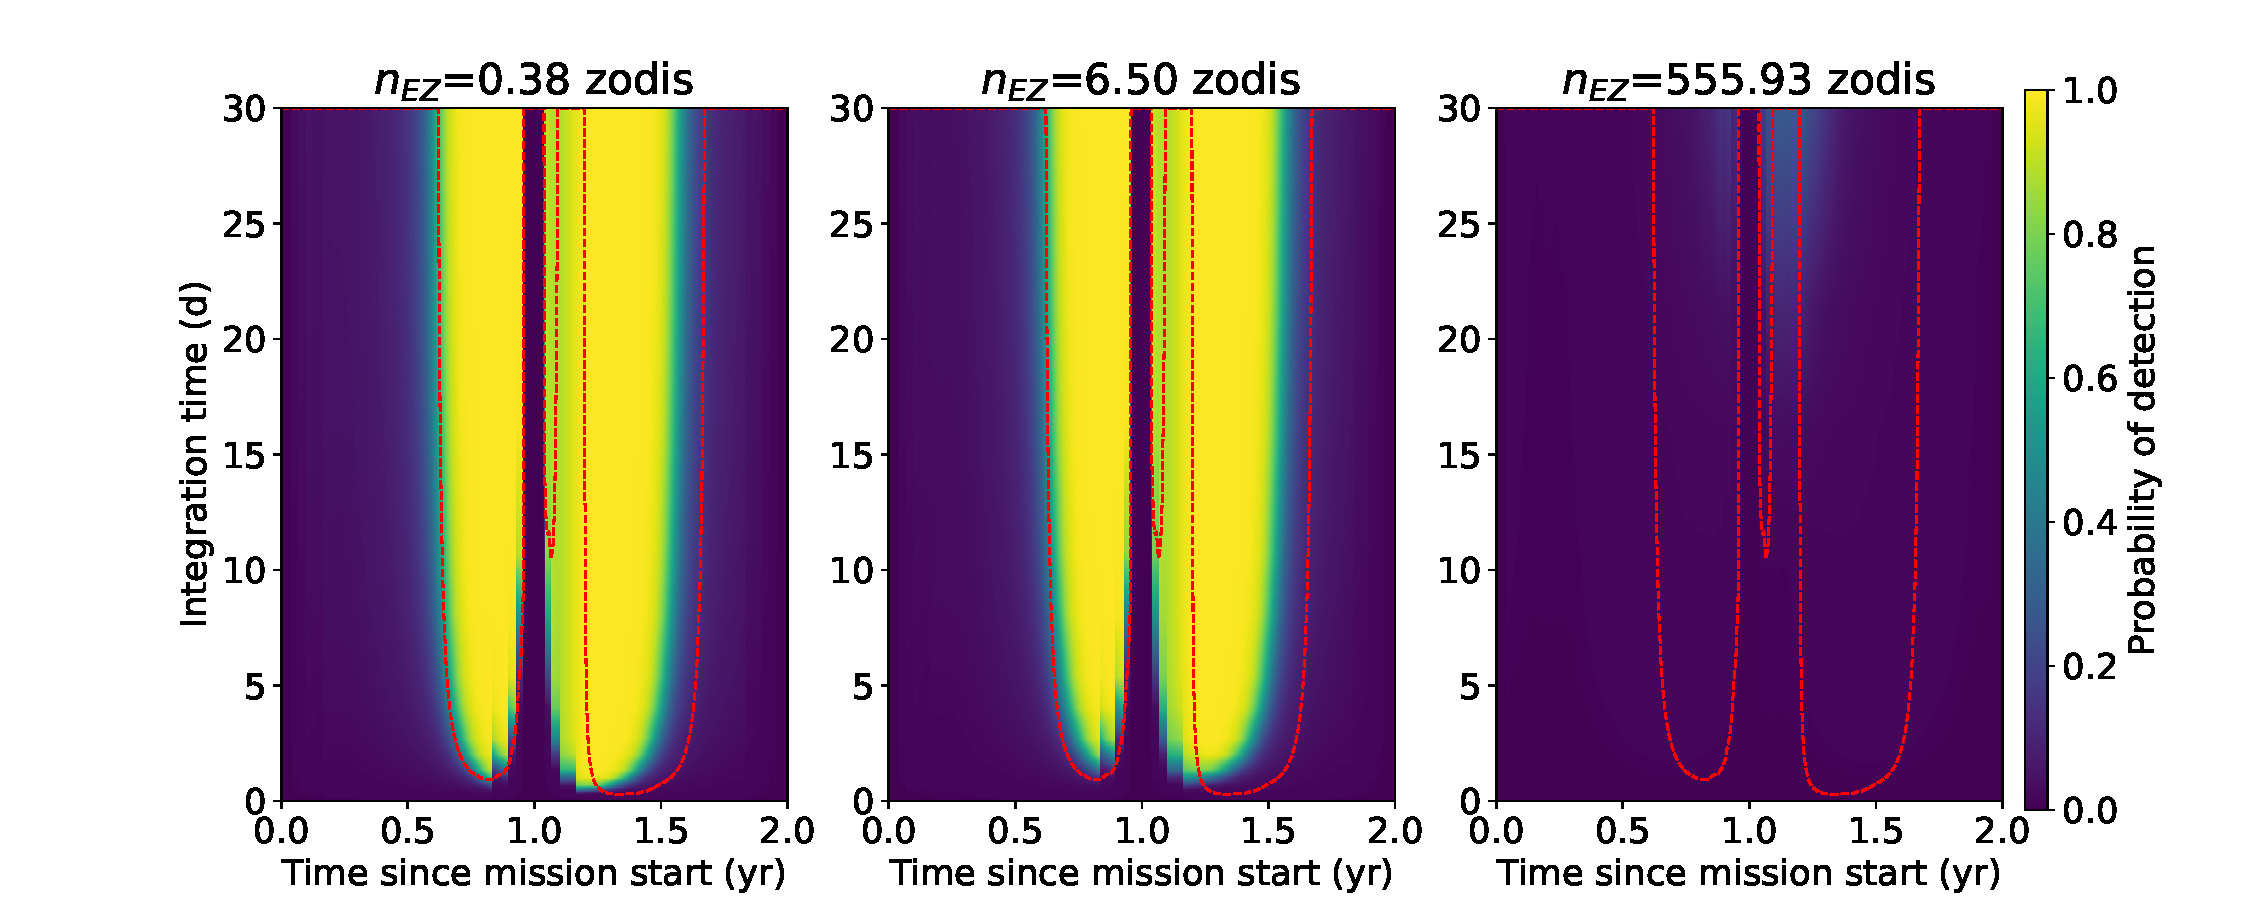
\includegraphics[width=0.95\textwidth]{ch3/figures/pdet_colored_true_overlay.pdf}
  \end{center}
  \caption{Probability of detection values for a 6m telescope similar to the
  projected Habitable Worlds Observatory from \citet{morganExplorationExpectedNumber2022a}
  with the radial velocity fit shown in \Cref{fig:rv_fit}. The
red dotted line represents the true detectability of the planet. Any
observation made outside of the red lines would result in a missed detection.}
  \label{fig:pdet_colored_true_overlay}
\end{figure}

\begin{figure}
  \begin{center}
    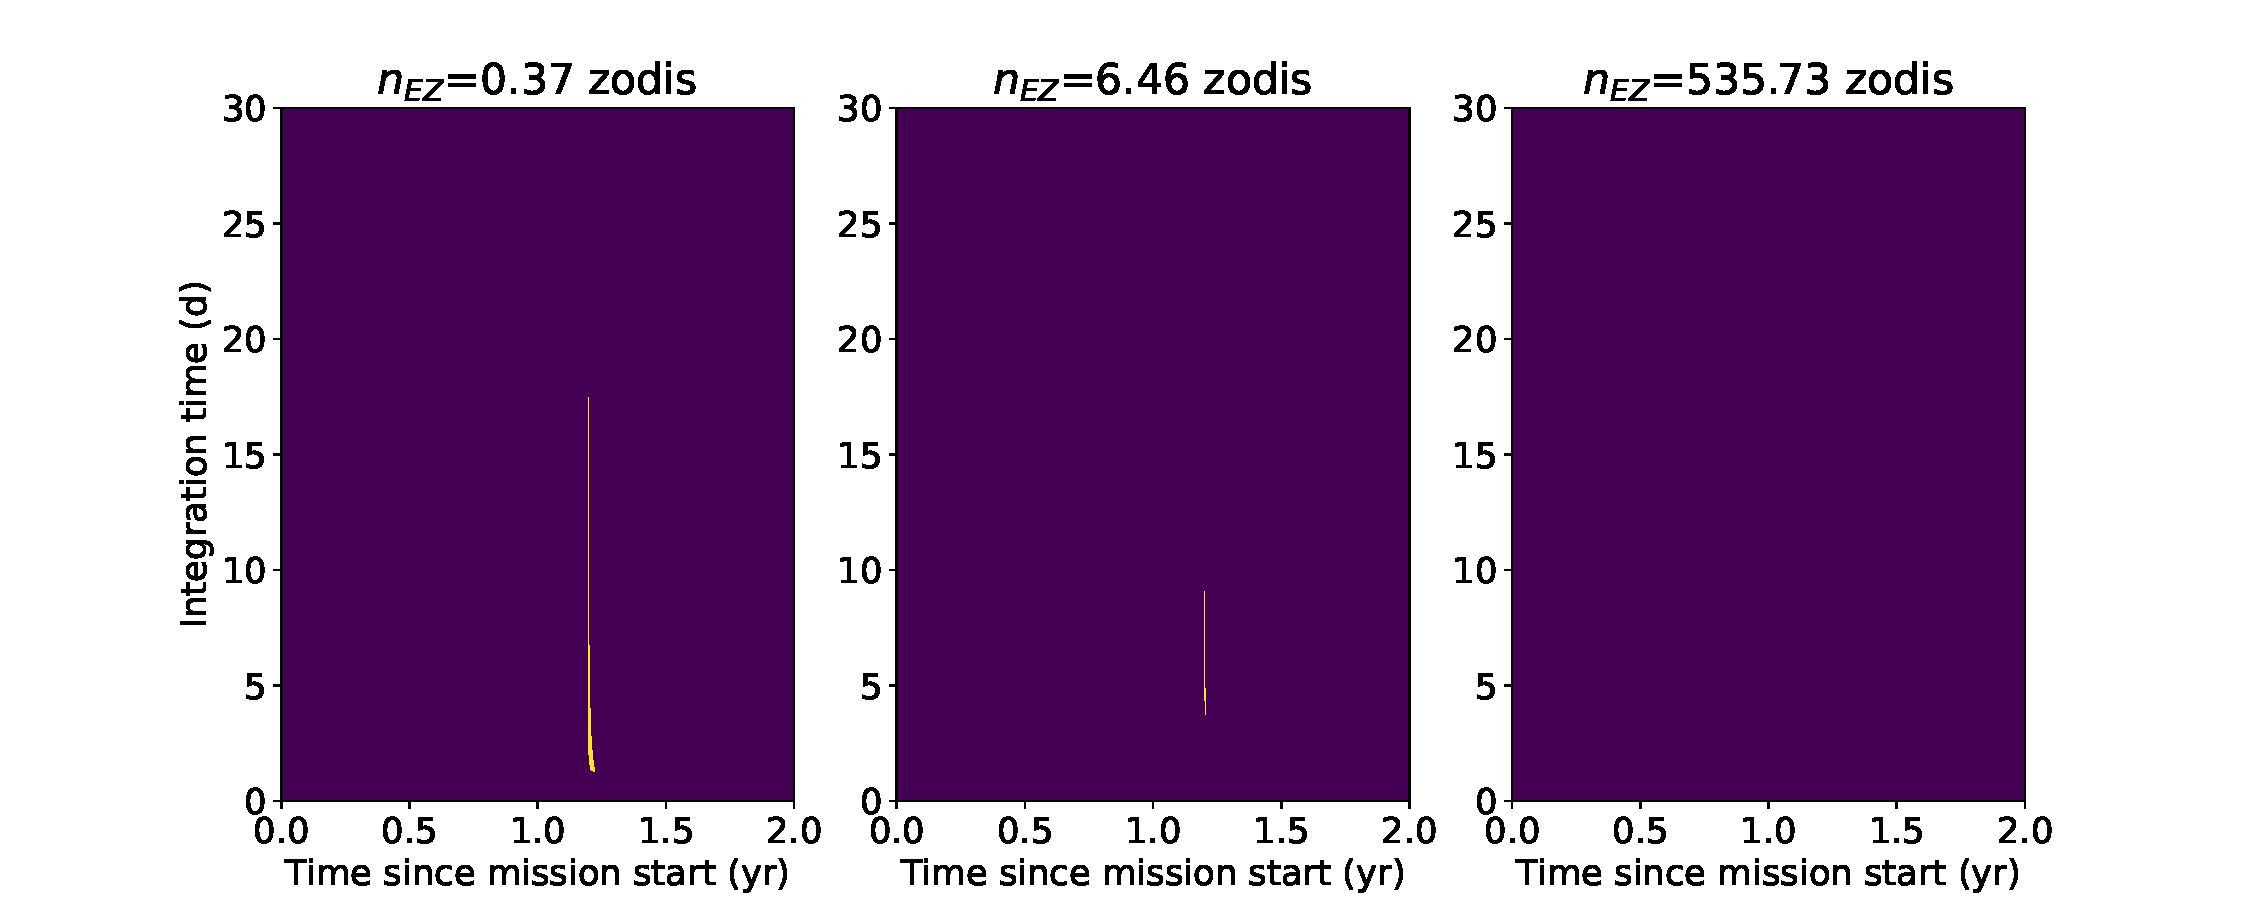
\includegraphics[width=0.95\textwidth]{ch3/figures/pdet_colored_true_err.pdf}
  \end{center}
  \caption{Plot highlighting where the estimated probability of detection is greater
  than 0.99 and the true planet is not detectable. Because very little of the space
  is highlighted this plot shows that the estimated probability of detection is a
  strong predictor of when the true planet is detectable. The only points highlighted
  correspond to when the true planet is exiting the IWA of the coronagraph which a
  scheduling algorithm could account for.}
  \label{fig:pdet_colored_true_err}
\end{figure}


To demonstrate the process we generated synthetic radial velocity data for a
randomly generated planet drawn from occurrence rates from
\citet{dulzJointRadialVelocity2020} fixed to be on a circular orbit. The true
planet parameters are $T=653$ days, $i=91.28\degree$, $M_p=0.79 M_\oplus$, $R_p
= 0.944 R_\oplus$. The RV data was created with precision $\sigma=0.03$ m/s.
The fitting was done with \code{RadVel} \citep{fultonRadvelRadialVelocity2018}
via the \code{RVSearch} package \citep{rosenthalCaliforniaLegacy2021} as shown in \Cref{fig:rv_fit}. A set of 10,000 orbits consistent with the RV
fit were created using the ``credible interval'' method from Chapter 2 and
propagated in time as shown in \Cref{fig:pop_propagation_in_time}.

The process of using the full photometric constraint from \Cref{sub:full_comp}
for $P_\textrm{det}$ gives us the probability of detecting the fitted planet as
a function of both observation and integration time, shown in
\Cref{fig:pdet_colored_true_overlay}. The plot includes the detectability of
the true planet, calculated using EXOSIMS, which shows strong agreement with
the calculated probability of detection based on the RV fit. The only major
section where the probability of detection is high and the planet is not
detectable is at the 1.1-year mark when the true planet is inside the inner
working angle. This is shown in \Cref{fig:pop_propagation_in_time} and while
the estimated probability of detection is high it is not unity, because the
sampling of orbital inclination described in Chapter 2 captures the fact that
only very edge-on orbits will be inside the inner working angle. We show the
areas where the calculated probability of detection is above 0.99 and the true
planet is not detectable in \Cref{fig:pdet_colored_true_err}, which shows that
the model does a very good job of capturing the true detectability of the
planet with only a small range of values where the model and the true
detectability do not line up while the planet is near the telescope's IWA.

\Cref{fig:pdet_colored_true_err} further shows how the assumption on
exozodiacal light impacts the resulting probability of detection, functioning
similar to a safety factor. Choosing a high $n_\textrm{EZ}$ value results in
lower probability of detection values in exchange for more guarantee that
any individual observation will be successful.

% section section:Observing scenario specific probability of detection (end)

\section{Conclusion} % (fold)
\label{sec:con_ddMag_comp}

In this chapter, we motivated the need to account for more astrophysical
parameters to estimate the probability of directly imaging a planet detected
with RV. We started by making an analogy to the completeness metric, a single
value to represent the likelihood of detecting a planet from an assumed
population given a specific star and mission design, to show that separation
and zodiacal light values have a considerable impact. If those effects are not
accounted for a yield study using summed completeness will systematically
overestimate the number of planets the mission will find. Then by calculating
$\Delta\textrm{mag}_0$ as a function of integration time, angular separation,
zodiacal light, and exozodiacal light, we showed that we can very accurately
estimate the observation and integration times necessary to directly image an
exoplanet. For a direct imaging mission scheduler this level of detail in the
probability of detecting a planet is very important because it shows the trade
space between the observing time and integration time available for a specific
target. Making an optimal schedule requires efficient use of observation time
and this process of calculating the probability of detection can be used to
increase the number of planets a direct imaging mission detects.

% section ch3_discussion (end)


\chapter{Scheduling with Simulated Precursor Data Collection for Direct Imaging Yield Modeling}
\label{cha:sim_and_scheduling}
\section{Introduction}
A major goal of the Habitable Worlds Observatory is to characterize the orbits
and atmospheres of as many habitable worlds as possible. To do this it will use
the direct imaging exoplanet detection technique since it provides the best
opportunity for full spectral characterizations. However, exoplanets are among
the faintest objects that have been the primary targets of an observation and
will require days to weeks of integration time. To complicate matters further,
multiple observations will be required to pin down the orbit of an exoplanet
before deciding on the best time to do a full spectral characterization.
Allocating the time required for spectral characterizations is therefore
incredibly costly given the considerable cost of construction, operation, and
alternative science objectives for a mission like the Habitable Worlds
Observatory.

Early in the life of a mission, many design decisions are driven by modeling
how the different aspects of a mission impact the science goals of a mission.
For exoplanets this can be seen in papers discussing the tradeoffs between the
diameter of the primary mirror and the number of exoplanets  that will be
detected, often called the "mission yield". Yield modeling studies will be
important to the success of the Habitable Worlds Observatory and two primary
tools have been created to study the mission yield of space-based direct
imaging missions, \code{EXOSIMS} and AYO. Both tools were built around calculating the
mission yield with no prior information about the planetary system of the
available target stars. However, it is likely that by the time of launch there
will be a considerable amount of information for some planetary systems.

Considerable effort is being invested into improving the radial velocity (RV)
exoplanet detection method to discover more exoplanets, and it has been
identified as the most promising method to detect Earth-like exoplanets. The
mission concept studies of both HabEx and LUVOIR identified the collection of
precursor RV data as integral to increasing the number of exoplanets detected.


The most recent study, \citet{morganExplorationExpectedNumber2022a}, showed
that having precise orbital information from RV before launch can improve yield
considerably [expand with study specifics]. This study is best thought of as an
upper bound for the mission yield improvement due to RV data because it assumed
full orbital recovery. Assuming full orbital recovery comes with many benefits
for computational time and is done probabalistically based on research on what
planets are likely to be discovered depending on the amount and quality of RV
data collected. This makes it a quick and robust way to determine which planets
are likely to be detected. 

The drawback of using full orbital recovery for yield modeling is that fitting
orbits to RV data only estimates certain orbital parameters. The standard set
is period $T$, time of conjunction $T_c$, argument of periapsis $\omega$,
eccentricity $e$, and minimum mass $M_p \sin{i}$. The minimum mass quantity
combines two parameters that impact direct imaging and estimations of an
exoplanet's brightness and location cannot be exact without separating the
planet mass and inclination. Without non-RV data those quantities cannot be
separated. An additional complication is that orbit fits have uncertainties on
fitted parameters which should be accounted for when scheduling observations.

A way of accounting for the inclination and mass ambiguity and uncertainty was
shown in \Cref{cha:first_paper}. The uncertainties from the fitting
process and an inclination prior are used to create a set of orbits that the
planet that created the radial velocity curve is most likely to be on. Then the
probability of detection is calculated, similar to the completeness metric
established in \citet{Brown2005d}, by propagating the orbits in that set and
comparing each orbit's brightness and planet-star separation to a direct
imaging telescope's sensitivity limits.

Fully simulating direct imaging missions with precursor RV requires simulating
the many RV observing runs that collect RV data for the stars in the direct
imaging target list. Real RV data cannot be used because the full planetary
systems that generate real RV data are unknown.

\section{Methods}
To incorporate precursor data realistically we must create synthetic planetary
systems around the stars in the simulation, simulate the collection of RV data,
do blind RV fitting of the RV data to create fits for scheduling, calculate the
probability of detection for each fit during the direct imaging mission, and
finally use the probability of detection information to create a direct imaging
observation schedule, and finally simulate the mission using a direct imaging
mission simulator. The major code pieces are \code{EXOSIMS} for planet generation and
direct imaging observation simulations, \code{RVSearch} for blind fitting RV data, and
the new package \code{RVtoImaging} that handles RV observations and scheduling. An
overview of the software package is shown in \Cref{fig:rv2imgflowchart}.

\begin{figure}
  \begin{center}
    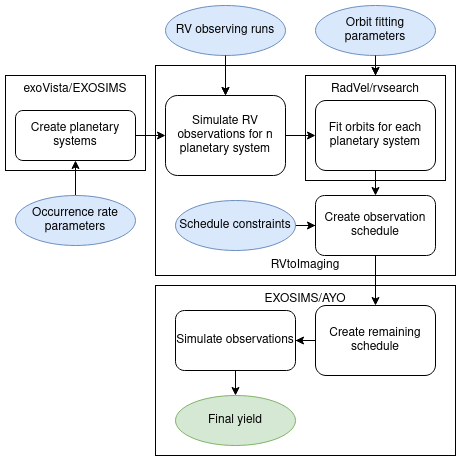
\includegraphics[width=0.95\textwidth]{ch4/figures/flowchartwhite.png}
  \end{center}
  \caption{Framework for simulating the use of precursor radial velocity data
  for direct missions.}
  \label{fig:rv2imgflowchart}
\end{figure}

The code is built to save anything that may be used again to reduce computation
time. It has detailed logging information printed for all steps of the process
and it manages a complex file structure to ensure that data can be quickly
found. Inputs are managed as a set of dictionaries from a driver script that is meant
to be easily modified.

\subsection{Planetary system generation}

The synthetic systems used in this study are created with \code{EXOSIMS}'s
implementation of the nominal occurrence rates from Dulz \citep{dulzJointRadialVelocity2020}. Full systems
are generated and then imported into a python package, exoverses, which was
created to work as an intermediary between planetary system generators and
\code{RVtoImaging}. Currently exoverses supports exoVista and \code{EXOSIMS}.

\subsection{RV Dataset}

The RV dataset is composed of user-defined RV observing runs and a set of
target stars. These observing runs are defined by
\begin{itemize}
  \item Bad weather probability
  \item Exposure time
  \item Min and max airmass
  \item Minimum observations per star
  \item Observatory location
  \item Start and end time
  \item RV precision terms
  % \item Observation scheme
\end{itemize}
This section of code makes uses the \code{astroplan} python package to
determine observability of the target stars for the observatory location and
airmass constraints \citep{morrisAstroplanOpen2018}. The simple observation
scheme takes in an average number of observations per star per year and assigns
those observations to discrete blocks that are equal in length to the exposure
time. Observations cannot overlap and stars are only observed once per night.
The constraint observation scheme is set up to simulate having a set number of
observing nights. Users define a set number of nights for observation and the
nights are drawn randomly within the given time frame. Then we set up an
optimization problem that maximizes the number of observations on each given
night and the number of stars that are observed a user-defined minimum number
of times, subject to the constraints that no star should be observed more than
once per night and no observations can overlap. The optimization problem is
solved using the Constraint Programming Satisfiability (CP-SAT) solver from
OR-Tools \citep{perronORTools2022}. After all observations are assigned, each
night gets a random draw of bad weather, if there is bad weather then the
observations from that night do not occur.

After a schedule is created we simulate the observation of the stars. For each
target we calculate the true anomaly, $\nu$, of all planets in the system and
calculate the star's radial velocity as 
\begin{equation}
v_s = \Sigma_i \left(K_i \left(e_i
\cos(\omega_i) + \cos(\nu_i + \omega_i)\right)\right) \,
  \label{eq:system_rv}
\end{equation}
where $K_i$, $e_i$,
$\omega_i$ are the RV semi-amplitude, eccentricity, and argument of periapsis
respectively of planet $i$. Each observing run is defined with a number of
error terms that are added in quadrature to get a final RV precision. Then we
treat the noise sources as uncorrelated and draw RV errors for each measurement
with the final RV precision as the one $\sigma$ value for a Gaussian
distribution centered on zero. There are time-correlated noise signals in real
RV data which can be corrected. However, this is done in a case-by-case basis
and is difficult to scale \citep{guptaTargetPrioritization2021}. Additionally,
we would be adding time-correlated noise with a Gaussian processes and then
removing them with the same Gaussian process analysis
\citep{aigrainGaussianProcess2022}. It is possible to deliberately chose
different kernel functions for the Gaussian process used in generation and the
Gaussian process used in fitting to add noise, but it is much more straight
forward to treat the time-correlated noise terms as a single value of RV
uncertainty to be defined by the user.

This process of generating RV data is repeated for each target star in the
observing run. Then the full process is repeated for every observing run in the
RV dataset. \code{RVtoImaging} is set up so that RV observing runs are deterministic
for a given generated universe and observing run parameters, allowing a user to
easily test how different combinations of observing runs impact fitting and
ultimately direct imaging scheduling. It is easy to compare how an individual
observing run impacts the final fit of a planetary system by adding or removing
it from the script driving the simulation.

\subsection{Blind RV fitting}

\code{RVtoImaging} does a blind search for every star with observations in the RV
dataset. A number of tools exist to do RV fitting, but systematic
blind searching without any prior information limits the number of tools. The
one best suited for this work is \code{RVSearch} which was created for the California
Legacy Survey \citep{rosenthalCaliforniaLegacy2021}. \code{RVSearch} is built on top of the radvel library, a python
package that uses the Markov Chain Monte Carlo (MCMC) simulations to fit
Keplerian orbits to RV data with confidence intervals. \code{RVSearch} sets up the
log-likelihood function as \citep{rosenthalCaliforniaLegacy2021} 
\begin{equation}
\ln(\mathcal{L}) = -\frac{1}{2}
\Sigma_i \left[ \frac{\left(v_i - m(t_i) - \gamma_D\right)^2}{\sigma_i^2} +
\ln\left(2 \pi \sigma_i^2\right)\right]
  \label{eq:likelihoodfun}
\end{equation}
where $i$ is the observation index,
$v$ is the RV measurement, $m$ is the model RV, $\gamma_D$ is the instrument's
offset, and $\sigma$ is the root-mean-square of error terms. The model is
defined as 
\begin{equation}
m(t) = \Sigma_n K(t|K_n,P_n,e_n,\omega_n,T_{c,n}) +
\dot{\gamma}(t-t_0) + \ddot{\gamma}(t-t_0)^2
  \label{eq:rv_model}
\end{equation}
where $n$ is the fitted orbit
index, $K(t|K_n,P_n,e_n,\omega_n,T_{c,n})$ is the RV signal for planet $n$, $P$
is the period, $T_{c,n}$ is the time of conjunction, $\dot{\gamma}$ is a linear
trend term, $t$ is the time of interest, $t_0$ is a reference time, and
$\ddot{\gamma}$ is a quadratic trend term. \code{RVSearch} works by creating a
Bayesian information criteria (BIC) periodogram of the RV data to identifying
the strongest periodic signals. \code{RVSearch} calculates the BIC as 
\begin{equation}
BIC = k
\ln\left(n_{obs})\right) - 2\ln{\mathcal{L}}
  \label{eq:bic}
\end{equation}
where $k$ is the number of free
parameters and $n_{obs}$ is the number of observations. With the strongest
periodic signal identified it does a maximum *a posterior* fit to determine the
most likely Keplerian parameters for the planet that generated the periodic
signal. Planets are added to a collective posterior until there are no periodic
signals left that improve the BIC, or until it reaches the maximum number of
planets it is allowed to search for.

After all significant periodic signals in the RV data have been identified,
\code{RVSearch} refines them and determines confidence intervals by performing a MCMC
simulation with all planet parameters free. This MCMC process is done using the
emcee library \citep{emcee} which is a popular python implementation of the affine
invariant ensemble sampler \citep{Goodman2010}. This process is very computationally costly,
because the search space increases considerably with every new planet and the
periodogram does a maximum *a posterior* fit at every test period with all
parameters of previously added planets free.

\code{RVtoImaging} works on forked versions of \code{RVSearch} and \code{RadVel} that were created
for performance reasons. The \code{RVSearch} fork was created primarily because the
current \code{RVSearch} package is pegged to \code{RadVel} version 1.3.8 and does not work
with \code{RadVel} versions 1.4.x which improved performance by vectorizing a number
of calculations. Further, the fork modifies some class attributes so that
\code{RVtoImaging} can tell things such as whether the MCMC chains converged. The
\code{RadVel} fork has a number of minor optimizations and a major optimization in the
form of a C version of the log likelihood function that implements the fast
eccentric anomaly solver from orvara \citep{brandtOrvaraEfficient2021} which is
based on \citet{raposo-pulidoEfficientCode2017}. An experimental feature was
added to the RVS

There are two major bottlenecks in this process. The first is that MCMC does
not scale well with multiple cores because emcee exits parallelization every
time it checks for convergence. Because of this it is better to spawn multiple
processes that have between 5-10 cores because any benefit gained by
parallelizing the periodogram search is offset by the wasted time in MCMC. The
more limiting bottleneck is that MCMC convergence drops considerably as more
planets are added. An unconverged MCMC run will give biased confidence
intervals which are of primary importance for estimating when a planet is
detectable so we will not consider unconverged chains valid in this work.
Convergence is rare, less than 20\%, when the number of planets in the search
space is five or more. When running multi-planet fits we found it best to cap
the number of planets in the search to four, which results in a 57\%
convergence rate and a standard run time of 30-40 minutes per search.

A major drawback of those computational limitations is that as more planets are
identified the parameter distributions of all planets become better
constrained. Additionally, by capping the number of planets fitted per system
to four we limit the number of planets we will consider in the scheduling step,
lowering the maximum yield. This is an unfortunate limitation because it restricts
our ability to fully understand the impact of different RV precision value.
This limitation is a necessary consequence of fitting tools prioritizing
precision over efficiency.

\subsection{Probability of Detection}

Probability of detection is calculated in the manner laid out in
\Cref{cha:accurate_pdet} paper), which is an adaptation of the "completeness"
metric described in \citep{brownSingleVisitPhotometric2005} . Using the MCMC
chains from the fitting process we generate a representative sample of orbits
that are consistent with the observed RV data for each planet fitted. If the
fit is an accurate description of the consistent orbits, we can propagate the
consistent orbits in time and when they are all detectable the true planet will
be detectable as well. \code{RVtoImaging} is set up to work the "Credible Interval" or
the "Multivariate Gaussian" methods of constructing consistent orbits.
Calculating probability of detection relies on a specific set of direct imaging
observatory parameters, since an orbit is considered detectable if it meets the
criteria laid out in \Cref{cha:accurate_pdet} The $\Delta\textrm{mag}_0(\alpha,
t_{\textrm{int}}, n_\textrm{Z}, n_\textrm{EZ})$ values are found for a specific
telescope using \code{EXOSIMS}'s \code{calc\_dMag\_per\_intTime} function. 

We do not attempt to create interpolants for all four inputs to
$\Delta\textrm{mag}_0$, instead calculating a 2d interpolant that takes in
$\alpha$ and $t_\textrm{int}$ values and returns the $\Delta\textrm{mag}_0$. An
interpolant is calculated for a discrete set of $n_\textrm{Z}$ values and a
single $n_\textrm{EZ}$ values. Extra zodiacal light brightness is a function of
the separation $\alpha$ and drops off with a $1/r^2$ term as discussed in
\citet{starkMaximizingExoEarthCandidate2014} so at every separation $\alpha$ we
calculate the corresponding extra zodiacal light surface brightness. Then when
calculating the $\Delta\textrm{mag}_0$ values at an observation time $t$ we
pick the interpolant that is closest to the current zodiacal light surface
brightness for the star at $t$, because it is a function of the telescope's
position in orbit, and the number of zodis assumed to be in the planetary
system. Ideally, we would be assigning the number of zodis in the system
probabilistically for each constructed orbit, but this is outside the scope of
this work as it adds a tremendous amount of complexity to the code. Instead we
treat the number of zodis in the planetary system as an input and assume it to
be constant when calculating the $P_\textrm{det}$ values for all planetary
systems.

In \code{RVtoImaging} the user defines an \code{EXOSIMS} input script for telescope
parameters, the consistent orbit construction method, a minimum integration
time, a maximum integration time, a start time, and an end time. Then the
orbits are repeatedly propagated between the start and end times and
$P_{\textrm{det}}(t, t_{\textrm{int}}, n_\textrm{Z}, n_\textrm{EZ})$ is
calculated for integration times spaced between the minimum and maximum. The
$P_{\textrm{det}}$ information for all planets around a star are stored as a
three dimensional array that is indexed on the planet number (assigned during
RV fitting), $t$, and $t_{\textrm{int}}$.

\subsection{Scheduling Observations}

Our aim in this work is to schedule observations of the fitted planets in a way
that is consistent with the observation strategies outlined in the HabEx and
LUVOIR studies \cite{gaudiHabitableExoplanetObservatory2020,TheLUVOIRTeam2019}.
They outlined a multi-tiered process that begin by using the telescope's
detection observing mode, as opposed to the observing mode for atmospheric
characterization, to better resolve the orbits of planets in the initial
portion of the mission. Work has shown that it takes 3-4 direct imaging
observations to determine an exoplanet's orbit to 10\%
\citep{bluntOrbitsImpatient2017}, and fewer are required when precursor data
exists \citep{gaudiHabitableExoplanetObservatory2020}. Further, it's important
to try and space out observations of a planet, as gathering 3 observations of
an Earth-like planet on 3 consecutive days will result in a considerably worse
fit than 3 observations made months apart. We use this information to drive our
scheduling task, attempting to get decent orbital coverage of as many fitted
planets as possible.

\subsubsection{The CP-SAT Solver}

Scheduling is done with a constraint programming tool, the CP-SAT solver from
OR-Tools\citep{perronORTools2022}. The methods behind the CP-SAT solver are
difficult to cite as it is developed by Google for internal use, but the code
itself is open source. Most of the information contained in this section has
been gathered by searching through the OR-Tools documentation
\url{developers.google.com/optimization}, the project GitHub, and various video
presentations given by the developers. At its core the CP-SAT is built to
transform a constraint programming (CP) problem into a satisfiability (SAT)
problem because better solvers have been developed for SAT problems. 

Constraint programming is defined by a set of variables and a set of
constraints. Each variable is assigned a finite range of values and constraints
are made on some subset of all the defined variables
\citep{shawConstraintProgramming2002}. The most common constraints are equality
relations between variables, however modern solvers provide many useful
abstractions such as conditional constraints, absolute value constraints, and
multiplication of variable constraints. Constraint programming is built around
the idea of finding a feasible solution rather than a necessarily optimal
solution because it is meant to work with very large sets of possible solutions
where finding an optimal solution is not computationally feasible. This does
not mean that it is unable to handle optimization though, as an objective
function to be minimized or maximized can be defined based on the variables in
the problem.

% Satisfiability problems consist of finding a variable assignement  fundamental 

% Using the CP-SAT solver is a combination of constraint programming, metaheuristics,


% There is frustratingly little documentation how exactly the CP-SAT solver
% works, as the developer recommendation is to a YouTube video.


\subsubsection{Decision variables}

Our decision variables are booleans $x_{i,
t, t_{\textrm{int}}}$ that are true (one) when star $i$ is observed starting at
time $t$ with integration time $t_{\textrm{int}}$, and false (zero) otherwise.
Large scheduling problems cannot be practically solved with continuous
variables, so \code{RVtoImaging} discretizes the times $t$ between the mission's start
and end into discrete observing blocks that the user input determines. Then the
integration times $t_{\textrm{int}}$ are set as multiples of the observing
block size. 

To improve the performance we take a number of steps to avoid creating $x_{i,
t, t_{\textrm{int}}}$'s that serve minimal purpose. Using the \code{EXOSIMS} script
that created the $P_{\textrm{det}}$ values we determine the keepout times and
only create an $x_{i, t, t_{\textrm{int}}}$ when the star is not in keepout.
The user sets a $P_{\textrm{det}}$ threshold and we create no $x_{i, t,
t_{\textrm{int}}}$ when all of the fitted planet's $P_{\textrm{det}}$ are below
the threshold. We loop through $t_{\textrm{int}}$ values from the least
to greatest and only create a new $x_{i, t, t_{\textrm{int}}}$ boolean when the
increase in integration time would result in more of the star's planets being above
the $P_{\textrm{det}}$ threshold. For performance reasons the CP-SAT solver
only works on integer values, so we multiply all $P_{\textrm{det}}$ values by a
constant user-defined coefficient and cast the values as integers. While a
large coefficient will more accurately represent the true $P_{\textrm{det}}$
values, the use of a threshold does not require it, and we have found a
coefficient of 100 to be sufficient.

\subsubsection{Constraints}

The main benefit of the CP-SAT solver is its flexibility regarding constraints.
Obvious constraints for this work are that observations must be scheduled
between the start and end of the simulation and that observations must be
separated by at least the observation overhead time. Another constraint is the
maximum number of observations of a single star. Flexibility in how long we
wait between observations of a star is important for orbital coverage, so
\code{RVtoImaging} takes as input a minimum and maximum wait time between observations
of a star. We want to tailor the wait time to the fitted systems, so we start
with a wait time of one quarter of the period of the planet with the shortest
fitted period. That wait time is used if it is within the range of the min and
max wait times, and is cut to the bounds if they are exceeded.

Adding all of these constraints as linear equations over the booleans $x_{i, t,
t_{\textrm{int}}}$ gets complicated quickly. To make constraints easier to
express we use an abstraction that OR-Tools provides called an "Optional
Interval Variable", which are defined by an integer "start" variable
$c_\textrm{start}$, an integer "size" variable $c_\textrm{size}$, and a boolean
"active" variable $c_\textrm{active}$. These intervals can be made to represent
an observations by mapping the discrete $t$ values to the $c_\textrm{start}$
variable and the discrete $t_\textrm{int}$ values to the $c_\textrm{size}$
variable. Interval variables map onto observations of a single star. Intervals
are effectively "off", they are not considered in constraints, when their
$c_\textrm{active}$ variable is false. We only create as many intervals as is
required per star, the minimum value between the user-set maximum observations
per star and the product of the number of fitted planets around a star and the
requested number of observations per planet. We connect the decision variables
to the interval variables using channeling constraints, intermediate boolean
variables that allow if-then style relationships. This forces a decision
variable to be true when an interval's $c_\textrm{active}$ variable is true and
its $c_\textrm{start}$ and $c_\textrm{size}$ values match the decision
variable's $t$ and $t_\textrm{int}$ values.

\subsubsection{Objective Function}

The decision variables $x_{i, t, t_{\textrm{int}}}$ are used because they can
be correlated to the $P_\textrm{det}$ values much easier than the interval
variables in the final objective function. Our goal here is not to simply
maximize the $P_\textrm{det}$ values, it is to improve the fits of as many
planet orbits as we can. Because of this we set up an integer variable for each
fitted planet, $b_\textrm{planet}$, that is equal to the number of observations
of the planet's star that occur at a time when the fitted planet is at or above
the user-set $P_\textrm{det}$ threshold. The $b_\textrm{planet}$ variables are
bounded at the user-input number of observations per planet. The final
objective function is stated as 
\begin{equation}
  \max{\left\{ \Sigma\left(W \cdot
  b_\textrm{planet}\right) - \Sigma\left( c_\textrm{active}\right) - \Sigma\left(
  c_\textrm{size}\right) \right\}}
  \label{eq:final_obj_function}
\end{equation}
where $W$ is a large weight term. The
$c_\textrm{active}$ terms are added to prevent observations with no benefit
from being included. The $c_\textrm{size}$ terms are there to reduce the
integration times if doing so does not affect the $b_\textrm{planet}$ term.
With the constraints and the objective function added to the CP-SAT model we
can use the CP-SAT solver to find an observation schedule that maximizes the
objective function.

\subsubsection{Simulating Observations}

With a schedule created we can simulate observations of the synthetic planetary
systems that created the synthetic RV data by importing the systems into an
\code{EXOSIMS} SimulatedUniverse module and then running an \code{EXOSIMS}
mission simulation. The same \code{EXOSIMS} input script that was used to
generate the $P_\textrm{det}$ values is used for the mission simulation. This
may come across as overfitting, given that we are using the same tool to
estimate the probability of detection as we are to estimate the true
detectability. Strictly speaking this is not incorrect, however mission
simulation software is a continually evolving process of adding as much detail
as is realistically possible to simulate a direct imaging mission and
represents our current models of direct imaging. It will be a continually
moving target to keep the probability of detection model up to date with our
current understanding of what factors drive a planet's detectability. As they
become more complex so must the probability of detection model.

\section{Results}

For the study here we populated every star in the NETS target list
\citep{guptaTargetPrioritization2021}, a set of 100 high priority radial
velocity targets, with a planetary system drawn from the
\citet{dulzJointRadialVelocity2020} occurrence rates, redrawing the system if
an Earth-like planet was not included as a best-case scenario and to test how
well the scheduler performs with a large number of targets. The planets outside
of the habitable zone were not included in the radial velocity calculations as
fitting multi-planet systems increases the computation time by many orders of
magnitude and in a real-life scenario there would be manual vetting of the
individual fits instead of strictly blind searches. The radial velocity data
was generated using a hypothetical "Extreme Precision Radial Velocity" (EPRV)
instrument with $\sigma = 3$ cm/s at the Keck observatory. We gave the radial
velocity instrument 100 observing nights per year for 5 years, with an exposure
time per target of 20 minutes which is roughly in line with the NEID exposure
time \citep{guptaTargetPrioritization2021}. Because we are studying an
idealized instrument we set the bad weather probability to zero for the work.
We assume that the RV observations continue right up until the mission launch
to eliminate dispersion error which was described in \Cref{cha:first_paper}. We
set a schedule optimization goal of 100 observations per target star for the
radial velocity scheduler and allowed the scheduler 10 minutes to run.

After simulating the observations and generating the radial velocity fits as
described above we calculated the probability of detection values using 10000
orbits constructed with the "credible interval" orbit construction method
described in \Cref{cha:first_paper}. The orbits were propagated for two years,
the approximate combined time of the Earth-like survey by the HabEx team
\citep{gaudiHabitableExoplanetObservatory2020}. The probability of detection
values were calculated for 19 integration times spaced logarithmically between
the minimum integration time of one hour and the maximum integration time of 30
days. The mission was assumed to be on an L2 orbit and the local zodiacal light
was calculated as a function of the observation time and the star's position.
The number of "zodis" in the planetary systems was treated as a constant value
in these simulations but the change in surface brightness as a function of
separation was accounted for in our estimation of the probability of detection.

Finally the direct imaging scheduler was run with allowed integration times
of 6 hours, 1 day, 5 days, 10 days, and 30 days. The planet was to be considered
detectable if the probability of detection was equal to or above 0.95 and each
planet was to be observed 3 times if possible. Then we set the minimum required
wait time to re-observe a star to 10 days and the maximum required wait time to
a quarter of a year. The scheduler was allowed to run for two hours.

\begin{figure}
  \begin{center}
    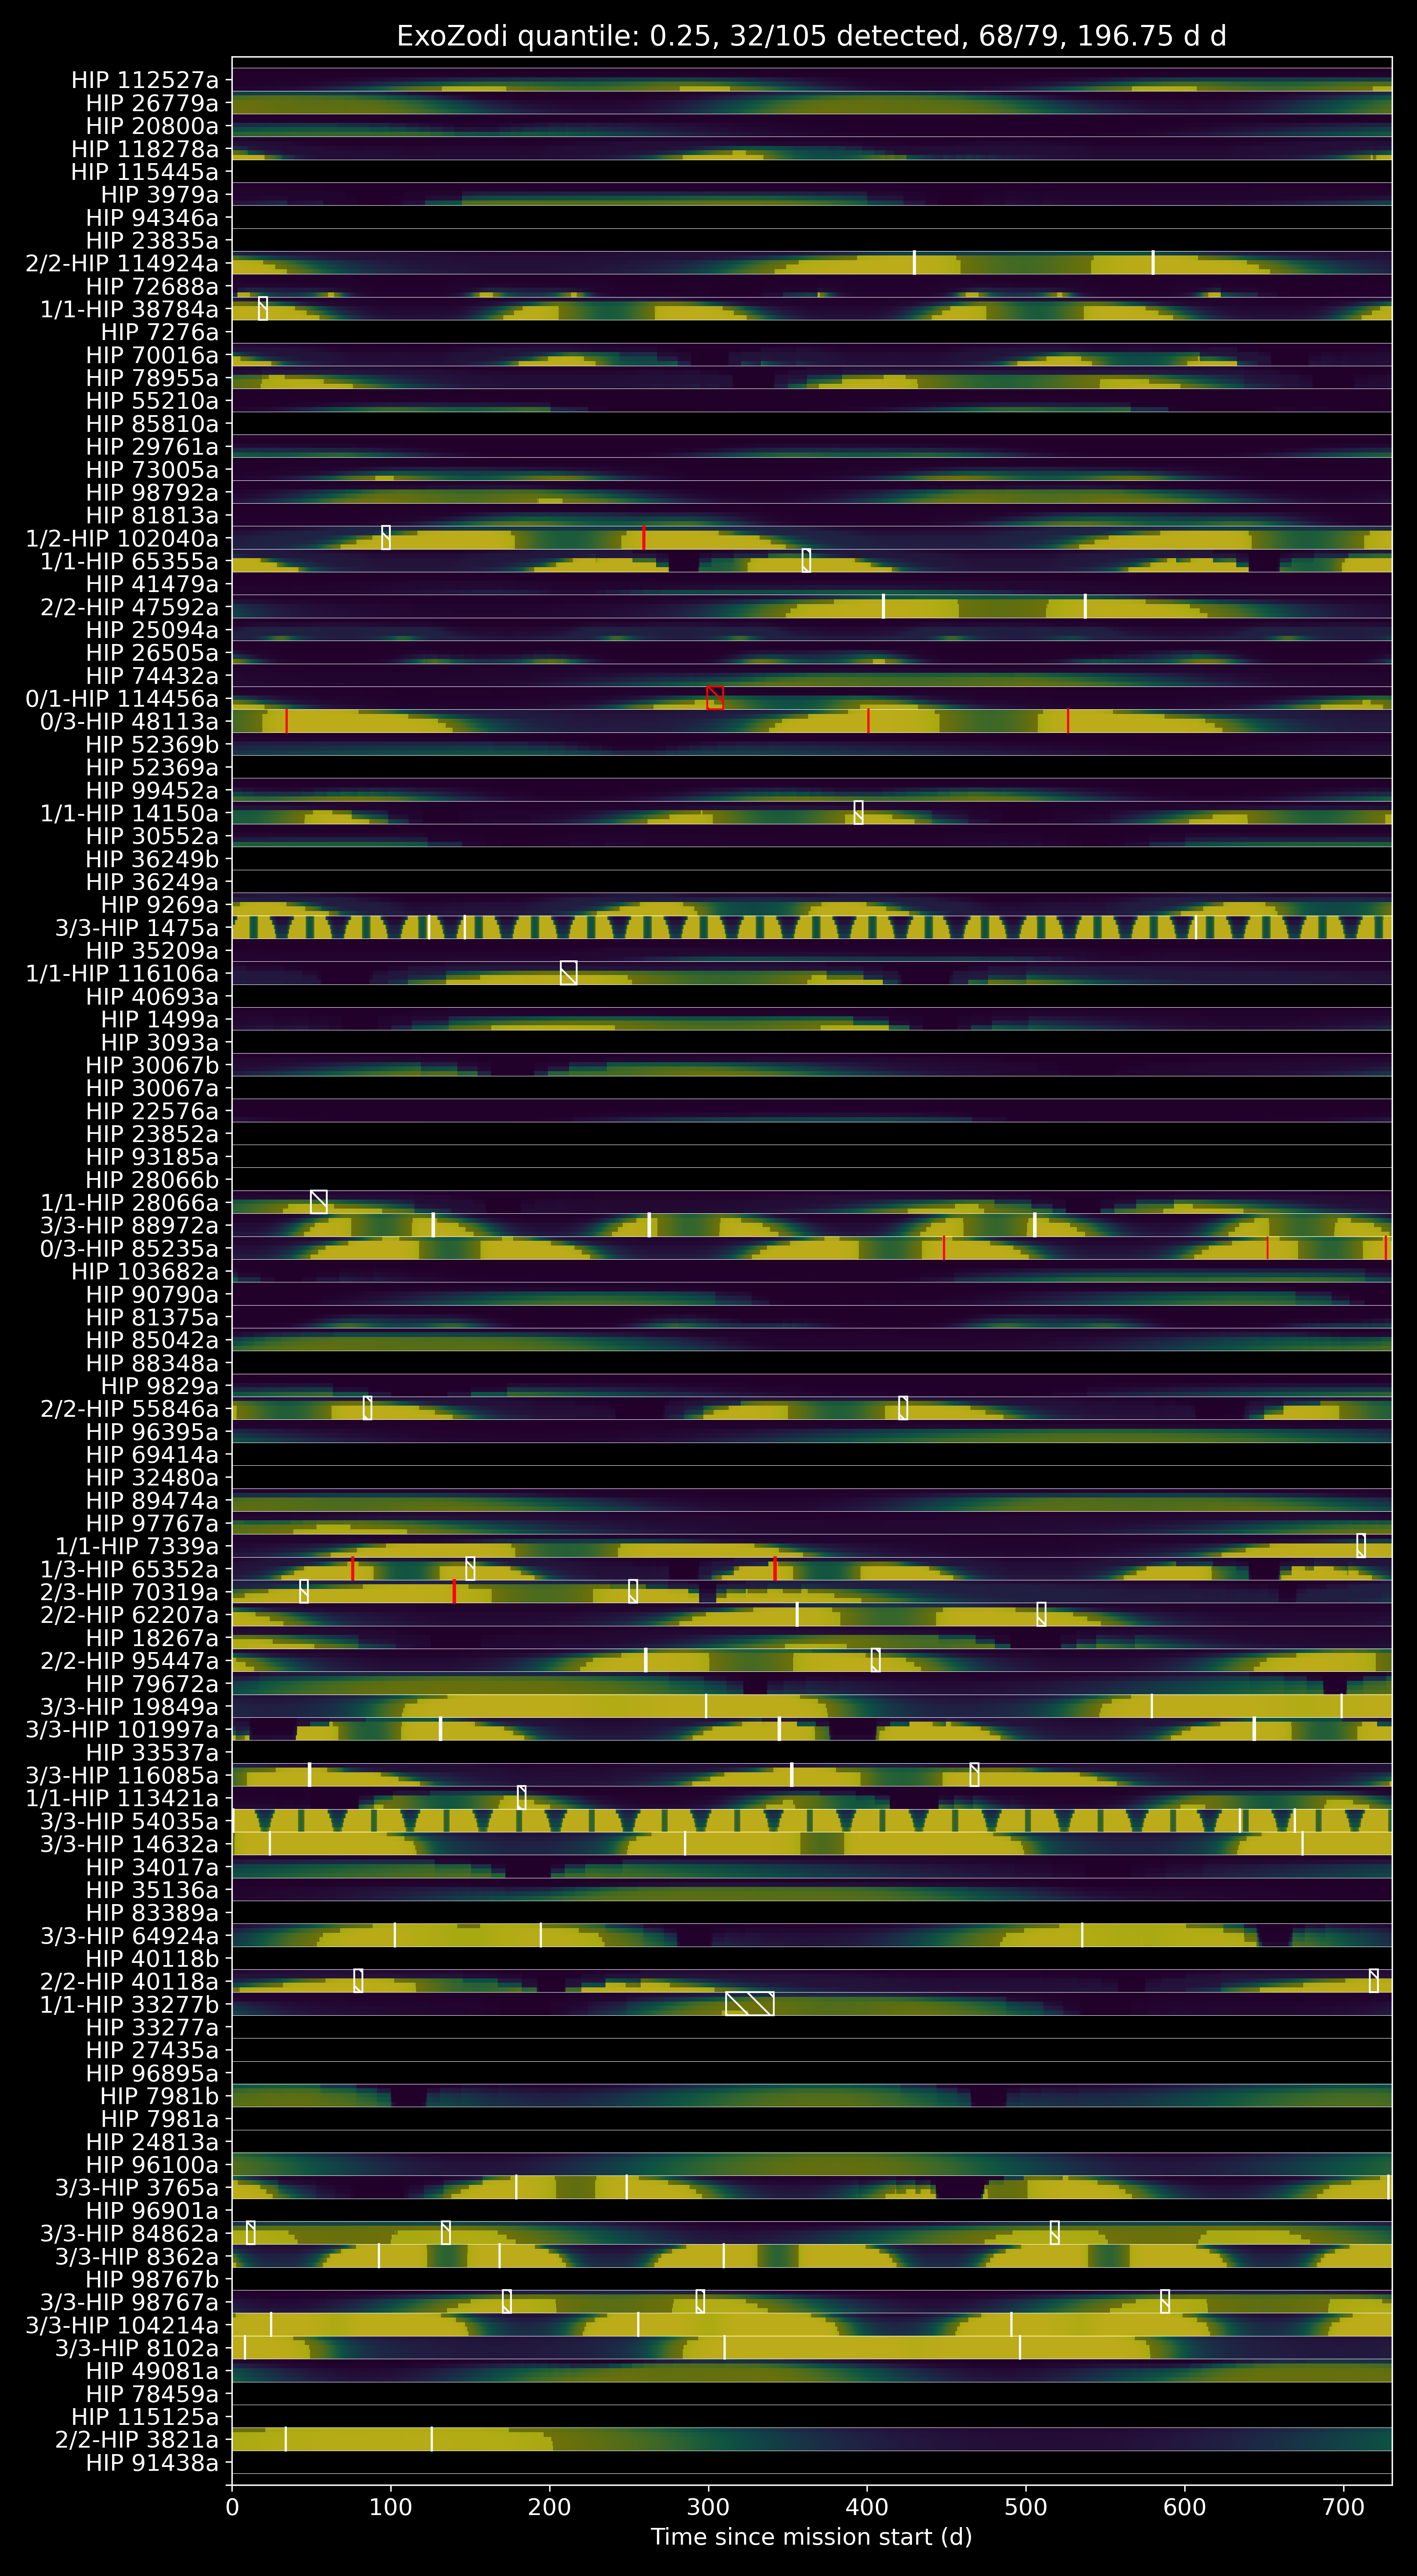
\includegraphics[height=0.9\textheight]{ch4/figures/schedule.png}
  \end{center}
  \caption{
    Schedule created based fits of 3 cm/s EPRV data on 97 stars populated with
    Earth-like planets.
  }
  \label{fig:schedule}
\end{figure}

\begin{figure}
  \begin{center}
    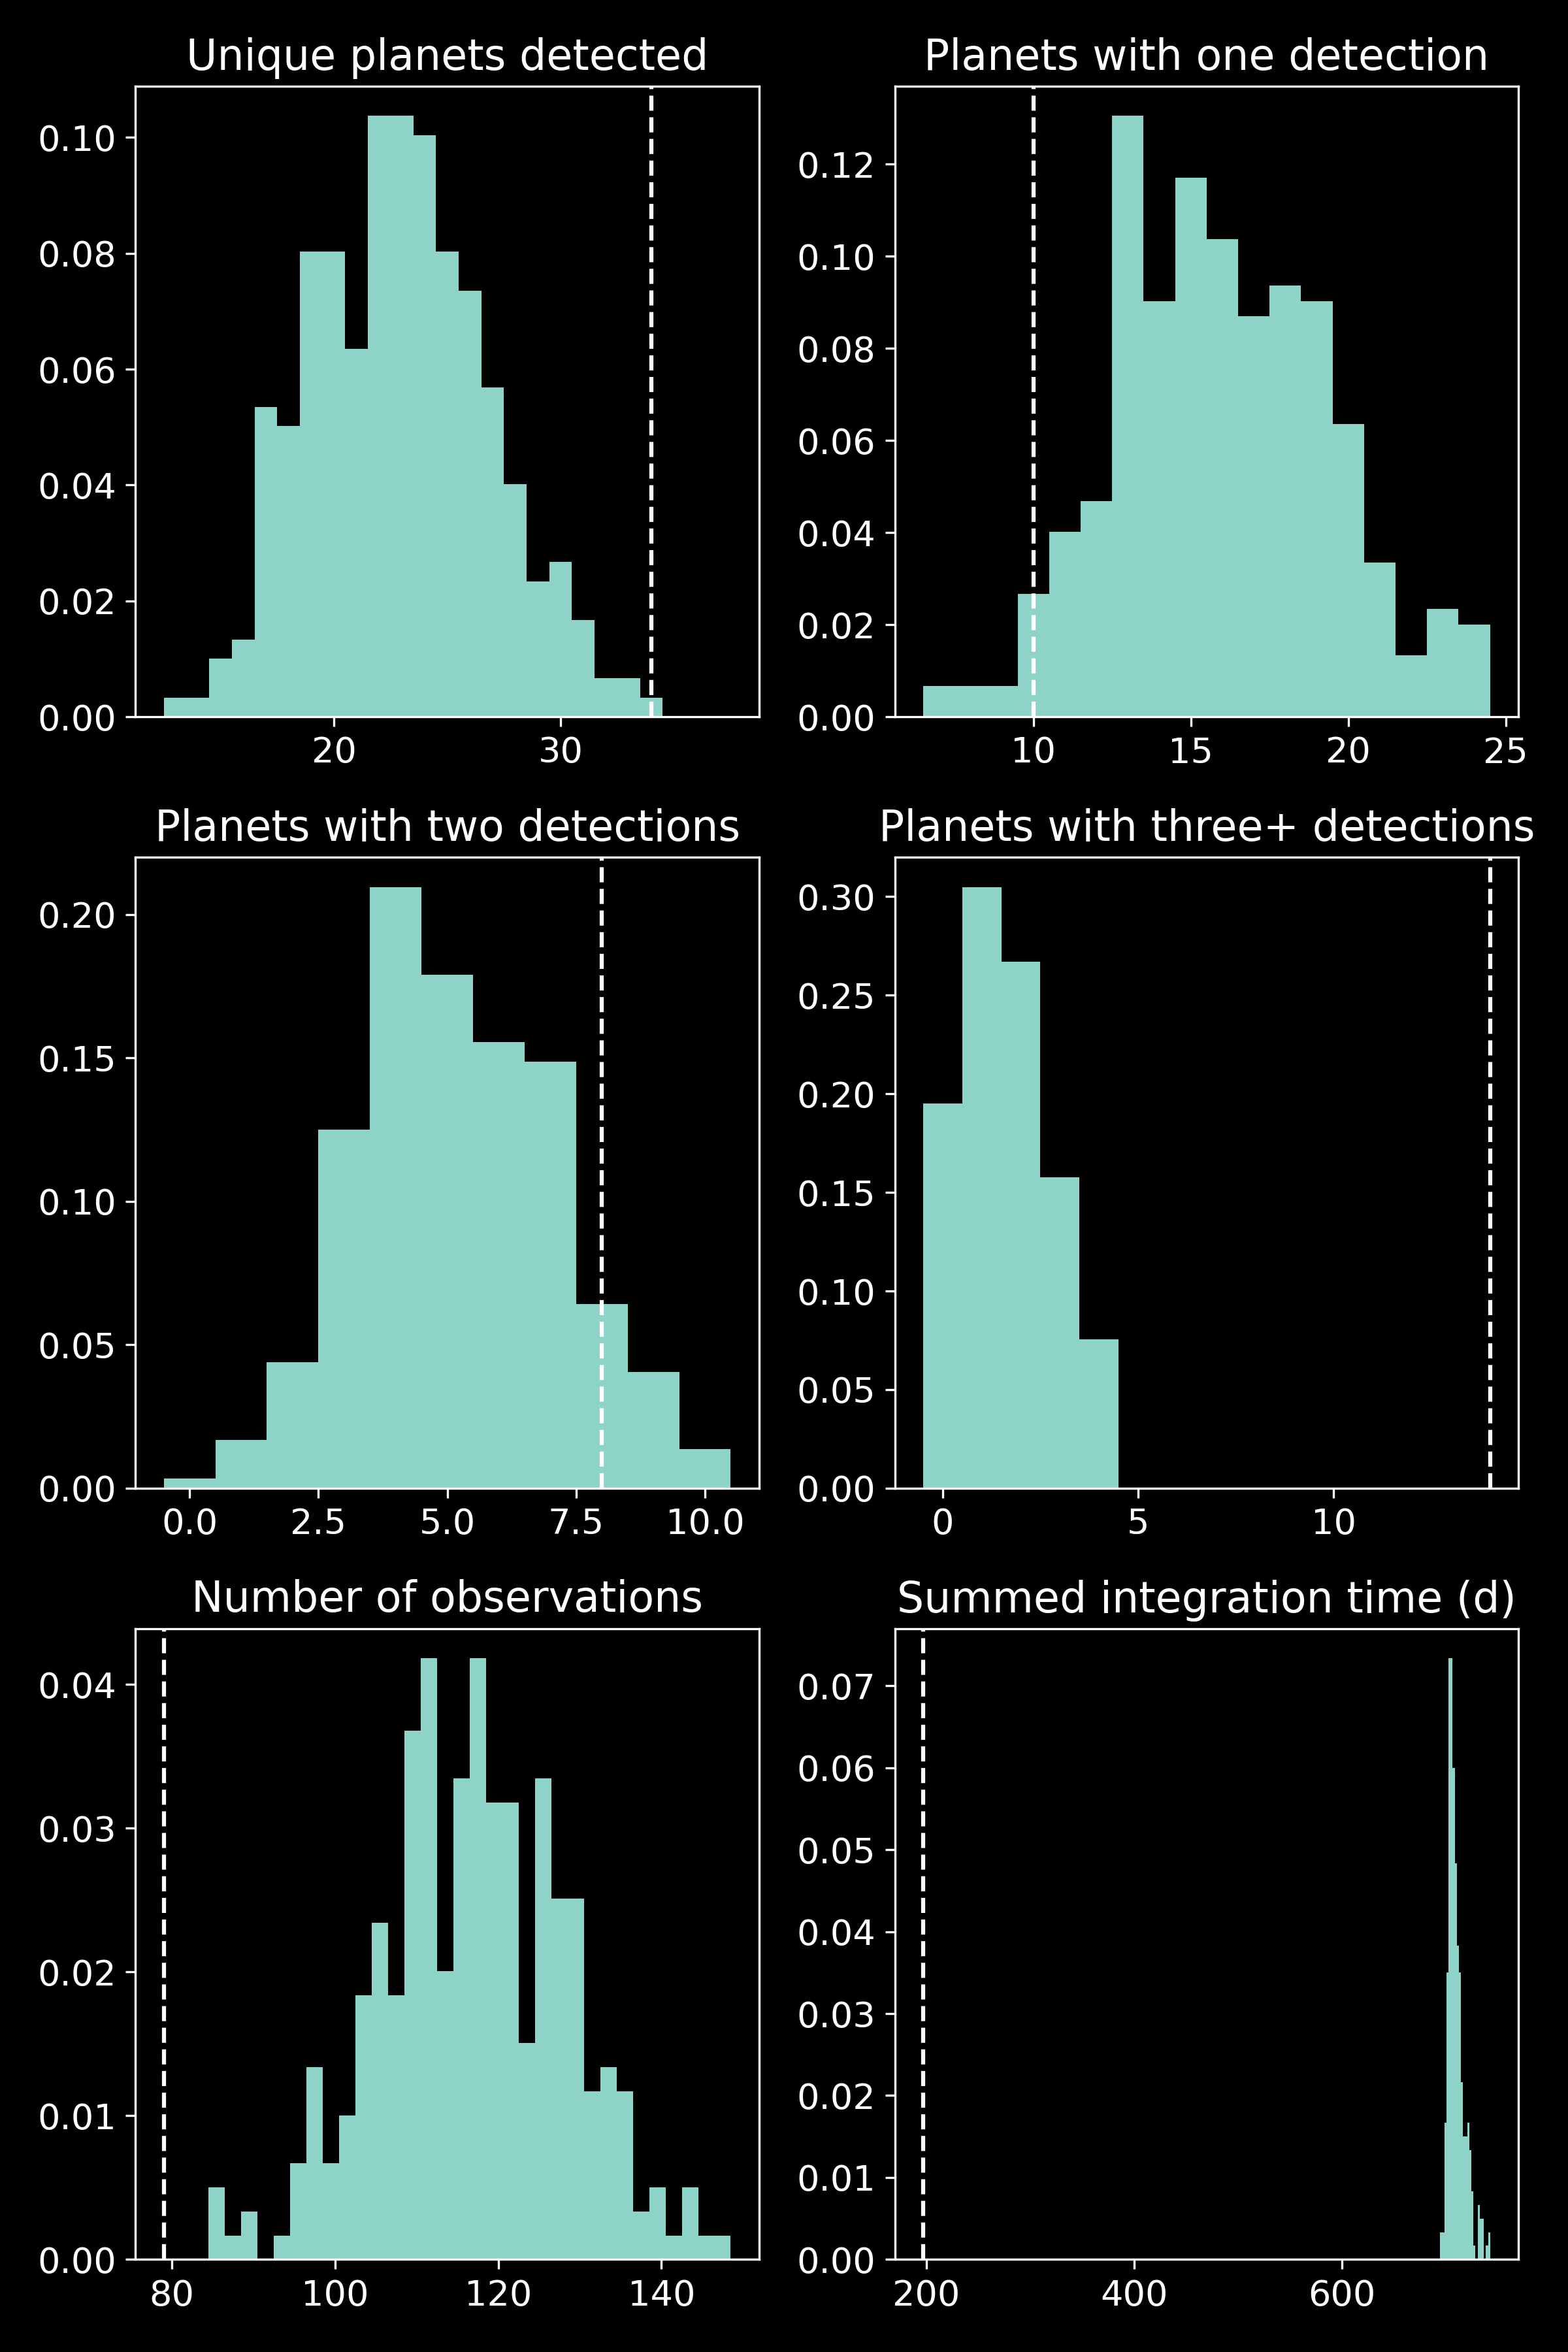
\includegraphics[height=0.75\textheight]{ch4/figures/hist.png}
  \end{center}
  \caption{Comparison between the static observing schedule, dashed line, set by the
  scheduler and a random walk between the 97 stars, histogram. All stars had an Earth-like planet,
  integration times were chosen to reach 25 $\Delta$mag (scaled by the stars luminosity).}
  \label{fig:randomwalkhist}
\end{figure}

An example schedule is shown in \Cref{fig:randomwalkhist}, where 32 of the 105
planets was detected at least once, 79 observations were scheduled, and 68 of
the scheduled observations were successful. In total the scheduler used 196.75
days of integration time out of the allowed two years. It is difficult to find
an analogous comparison in literature to the case we are showing, as previous
studies of RV knowledge fixed the positions of the planets to be the same for
all observations, used a much larger target list, and focused on full
characterization which is not included in this
work\citep{morganExplorationExpectedNumber2022a}. Because of this we compare
our schedule to a random walk scheduler, where we use the same set of planets
and telescope parameters and simulate a mission by choose the next target
randomly for the full mission time. The integration times per target star were
chosen such that instrument could reach $\Delta\textrm{mag}=25$. The results
can be seen in \Cref{fig:randomwalkhist} where our scheduler was able to detect
as many unique planets in 200 days of integration time as the random walk
scheduler detected with 700 days of integration time in its best case scenario.
Additionally the scheduler dramatically out performs a random walk in the
number of planets that it is able to detect three times.

To test the impact of the precision $\sigma$ and the assumed number of zodis in
a planetary system on the scheduler we ran the same situation without redrawing
until an Earth-like planet is in a system. In this way we end up with fewer
total fits, based on the occurrence rate of Earth-like planets,
$\eta_{\oplus}$, which we set to 0.24 in line with
\citep{dulzJointRadialVelocity2020} occurrence rates which was also used in the
EPRV study \citet{morganExplorationExpectedNumber2022a}. We reduce the
computation load as we are interested in the success rate of the fitting
algorithm and the scheduler. We testing the scheduler for 5 $\sigma$ values
(0.1, 0.07, 0.05, 0.03, 0.01 m/s) and 5 $q_\textrm{EZ}$ values (0.05, 0.25,
0.5, 0.75, 0.95) where the $q_\textrm{EZ}$ values map to zodi occurrence rates
used in the \code{EXOSIMS} module \code{Mennesson} based on
\citet{mennessonCONSTRAININGEXOZODIACAL2014} (CHECK with Dmitry that this is where
that fits file comes from). 

The results are shown in \Cref{fig:sigma_nEZ_impact_plots} where the impact of
the $\sigma$ value on the number of Exo-earths fitted is clearly demonstrated.
We see that if a 3 cm/s precision is reached, the value used in the EPRV study
\citet{morganExplorationExpectedNumber2022a}, then we can fit the orbits of
approximately 80 percent of the Earth-like planets. However, if we are limited
to 10 cm/s we will only expect to fit 40 percent of the Earth-like planets. By
then simulating the probability of detection, scheduling, and observation
process calculations we can study how the different $\sigma$ values impact
observation success rate and we see little effect. The $\sigma$
values strongly correlate to the percentage of planets detected, which is unsurprising
given that fewer orbits are fitted.

The assumed number of exozodi has a positive relationship with the observation
success rate and a negative relationship on the mission yield past the 50th
zodi quantile. This shows an interesting trade space where we can better
guarantee the success of an individual observation if we assume high levels of
extra zodiacal light, but this approach ultimately has a negative impact on the
total yield of the mission.

\begin{figure}
  \begin{center}
    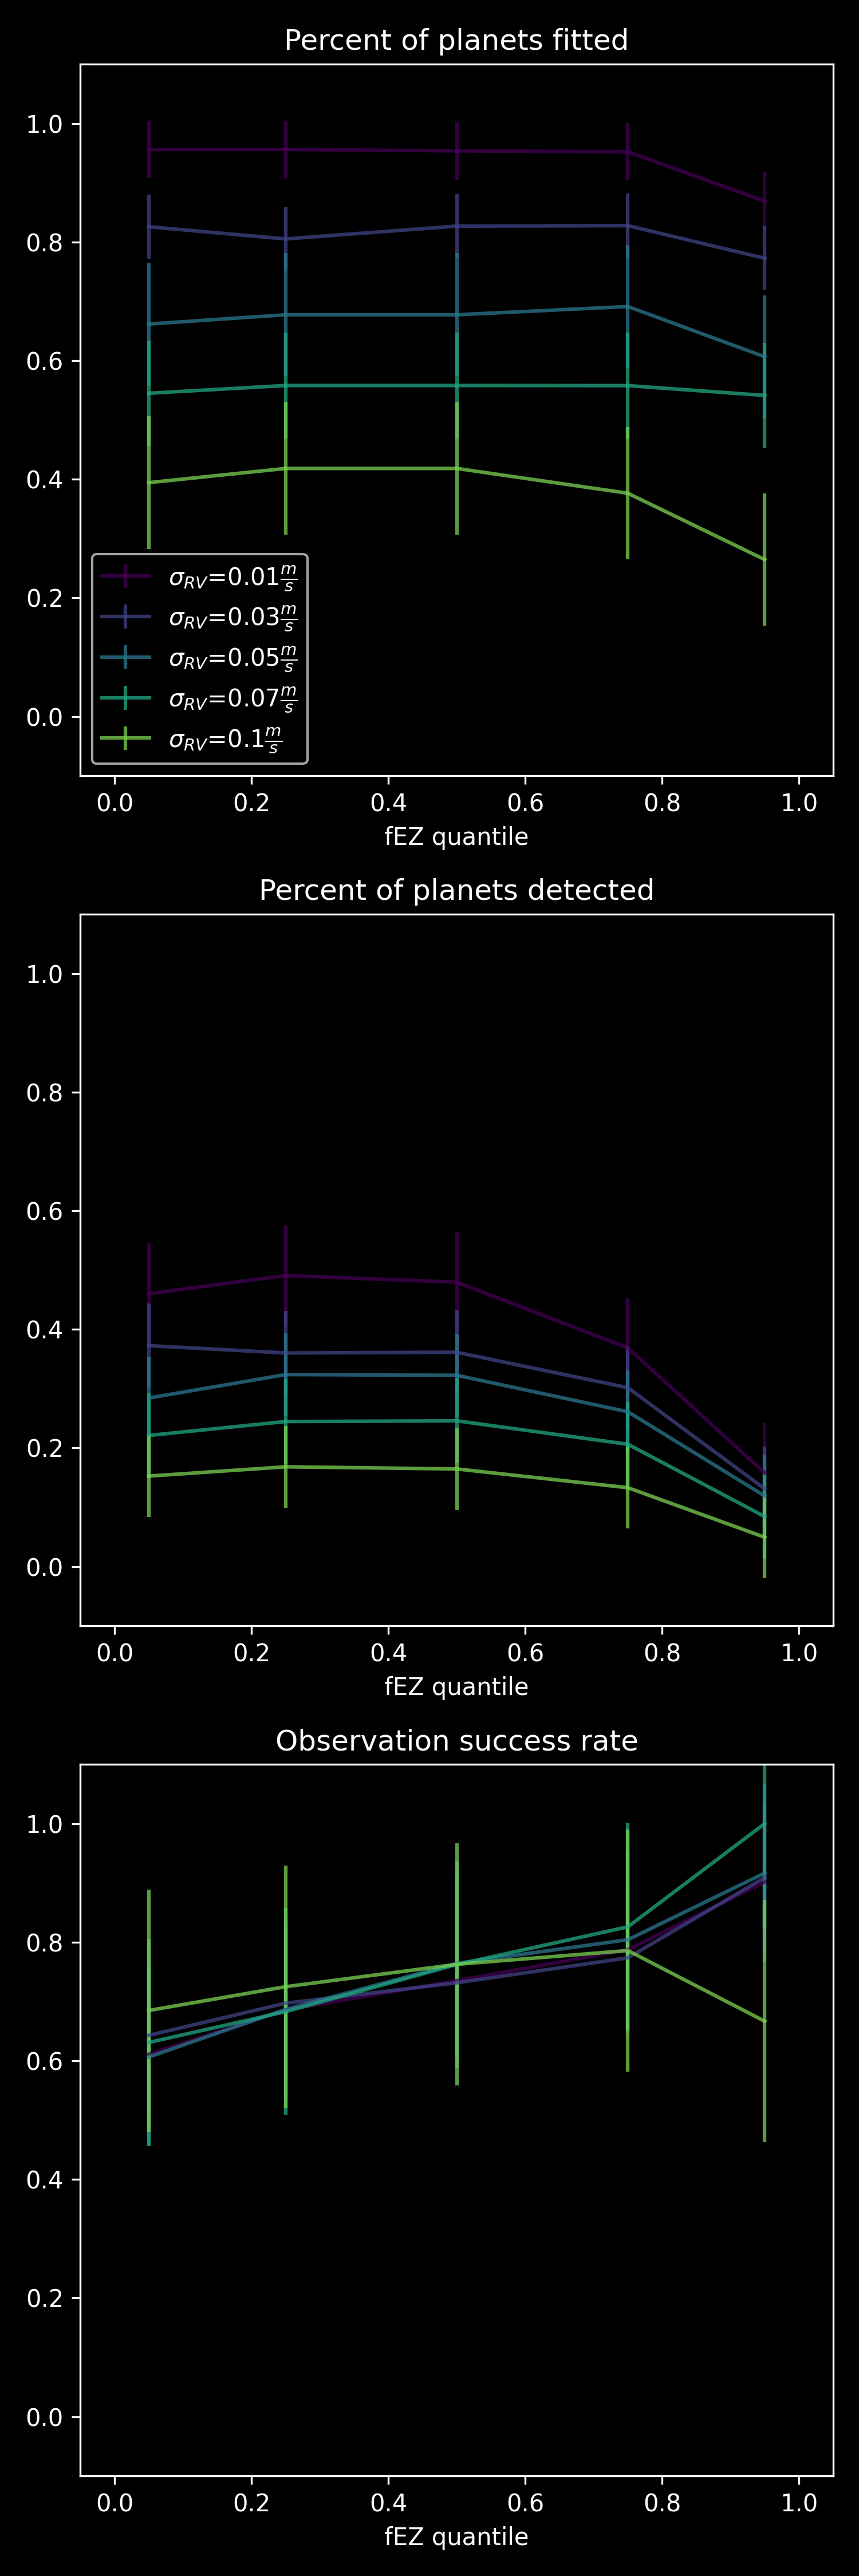
\includegraphics[height=0.9\textheight]{ch4/figures/fEZ_impact.png}
  \end{center}
  \caption{
    Impact of assumption on $\sigma$ and exozodi on scheduler results.
  }
  \label{fig:sigma_nEZ_impact_plots}
\end{figure}

\section{Conclusion}

In this chapter we have demonstrated a method of using constraint programming
to calculate an observing schedule that allows for dynamic variations in the
integration time and observation time for every planet with precursor radial
velocity data. To validate the scheduler we created a tool called \code{RVtoImaging}
that realistically simulates the RV data collection and fitting process,
calculates the probability of detection for a given orbit fit and direct
imaging telescope, schedules observations based on that data, and then uses
mission simulation software to test the scheduled observations. We showed that
our scheduler dramatically out performs a random walk scheduler. This work
proves that we can use the probability of detection metric to schedule direct
imaging observations of exoplanets detected via radial velocity and it shows
how precursor data can be incorporated in direct imaging mission yield
modeling.

More generally, by creating a flexible framework that does full simulations of
the RV observations and fitting process we have created a tool that can answer
many interesting questions in the use of precursor science for a flagship
direct imaging mission such as the Habitable Worlds Observatory. We used a
relatively simple setup in this chapter: a single observing run, no bad
weather, only planets in the habitable zone, and observations were continued
until the direct imaging mission launch. Future work will be on more
complicated scenarios, such as: how many EPRV observations of a planetary
system are required to accurately calculate probability of detection, how does
the planetary occurrence rate model impact which planets are ultimately fitted
via radial velocity, how do different RV orbit fitting tools compare, is there
there a benefit to prioritizing RV observations of stars with low completeness
because a blind direct imaging search will be more sensitive to that star.



% \chapter{Estimating the Covariances on Reported Planet Parameters (?)}

\appendix
\chapter{Chapter 1 of appendix}
Appendix chapter 1 text goes here

\bibliography{library}

\end{document}
